%-------------------------------------------------------------------
\chapter{Results}
\label{c:results}
%-------------------------------------------------------------------

This chapter summarises the main results of the thesis. It focuses on what we learned about Mixture Neural Cellular Automata (MNCA) for modelling tissue-like dynamics, and in particular on the role of the spatial neighbourhood size (\(NB\)). Experimental setups and implementation details are described in \cref{c:implementation}; here we concentrate on the figures, tables, and their interpretation.

%-------------------------------------------------------------------
\section{NB size effects in synthetic tissue models}
\label{sec:results:neighborhood}
%-------------------------------------------------------------------

Across the synthetic experiments, the evidence consistently indicates that \textbf{neighbourhood size is not a marginal hyperparameter}: it changes stability, long-horizon behaviour, and the trade-off between matching global statistics and reproducing spatial structure.
With minimal context (\(NB=1\), each cell sees only itself) the model is inadequate for the task; the analysis therefore focuses on \(NB \ge 2\).
In the controlled neighbourhood sweep (Step~3, \cref{sec:impl:step3:results}), \textbf{Kruskal-Wallis tests return \(p < 10^{-4}\)} across all metrics for both Mixture NCA and Stochastic Mixture NCA, and post-hoc comparisons (against baselines \(NB=2\) and \(NB=3\)) show that multiple neighbourhood sizes differ significantly from each other.

The main finding is that \textbf{once \(NB \ge 2\), performance does not improve monotonically with neighbourhood size}.
Different neighbourhood sizes lead to different compromises, and the ``best'' setting depends on (i) which metric is prioritised and (ii) the rollout horizon used for evaluation.

\subsection{Step 3: detailed trends across neighbourhood sizes}
\label{sec:results:step3}
%-------------------------------------------------------------------

In Step 3 we trained Mixture NCA and Stochastic Mixture NCA on \textbf{300 ground-truth histories of length 100}, one model per neighbourhood size \(NB \in \{1,\dots,7\}\), and evaluated them at three rollout horizons (Step Length \(=25, 50, 100\)).
For each configuration (model, \(NB\), step length) we computed six biological metrics on the final generated state (KL divergence, Chi-square, categorical MMD, tumour size difference, border size difference, spatial variance difference), averaged them across runs, and also inspected their per-simulation distributions.

Figure~\ref{fig:impl:step3:dashboard} reports the mean and variability of all six metrics across neighbourhood sizes.
The main qualitative pattern is consistent across metrics: \(NB=1\) is systematically inadequate, while moving to \(NB\ge2\) yields a sharp performance improvement.
Beyond this first jump, increasing \(NB\) produces a non-monotonic trade-off between matching global distributions (e.g., KL divergence) and matching spatial structure (e.g., tumour size and border properties).

\begin{figure}[H]
  \centering
  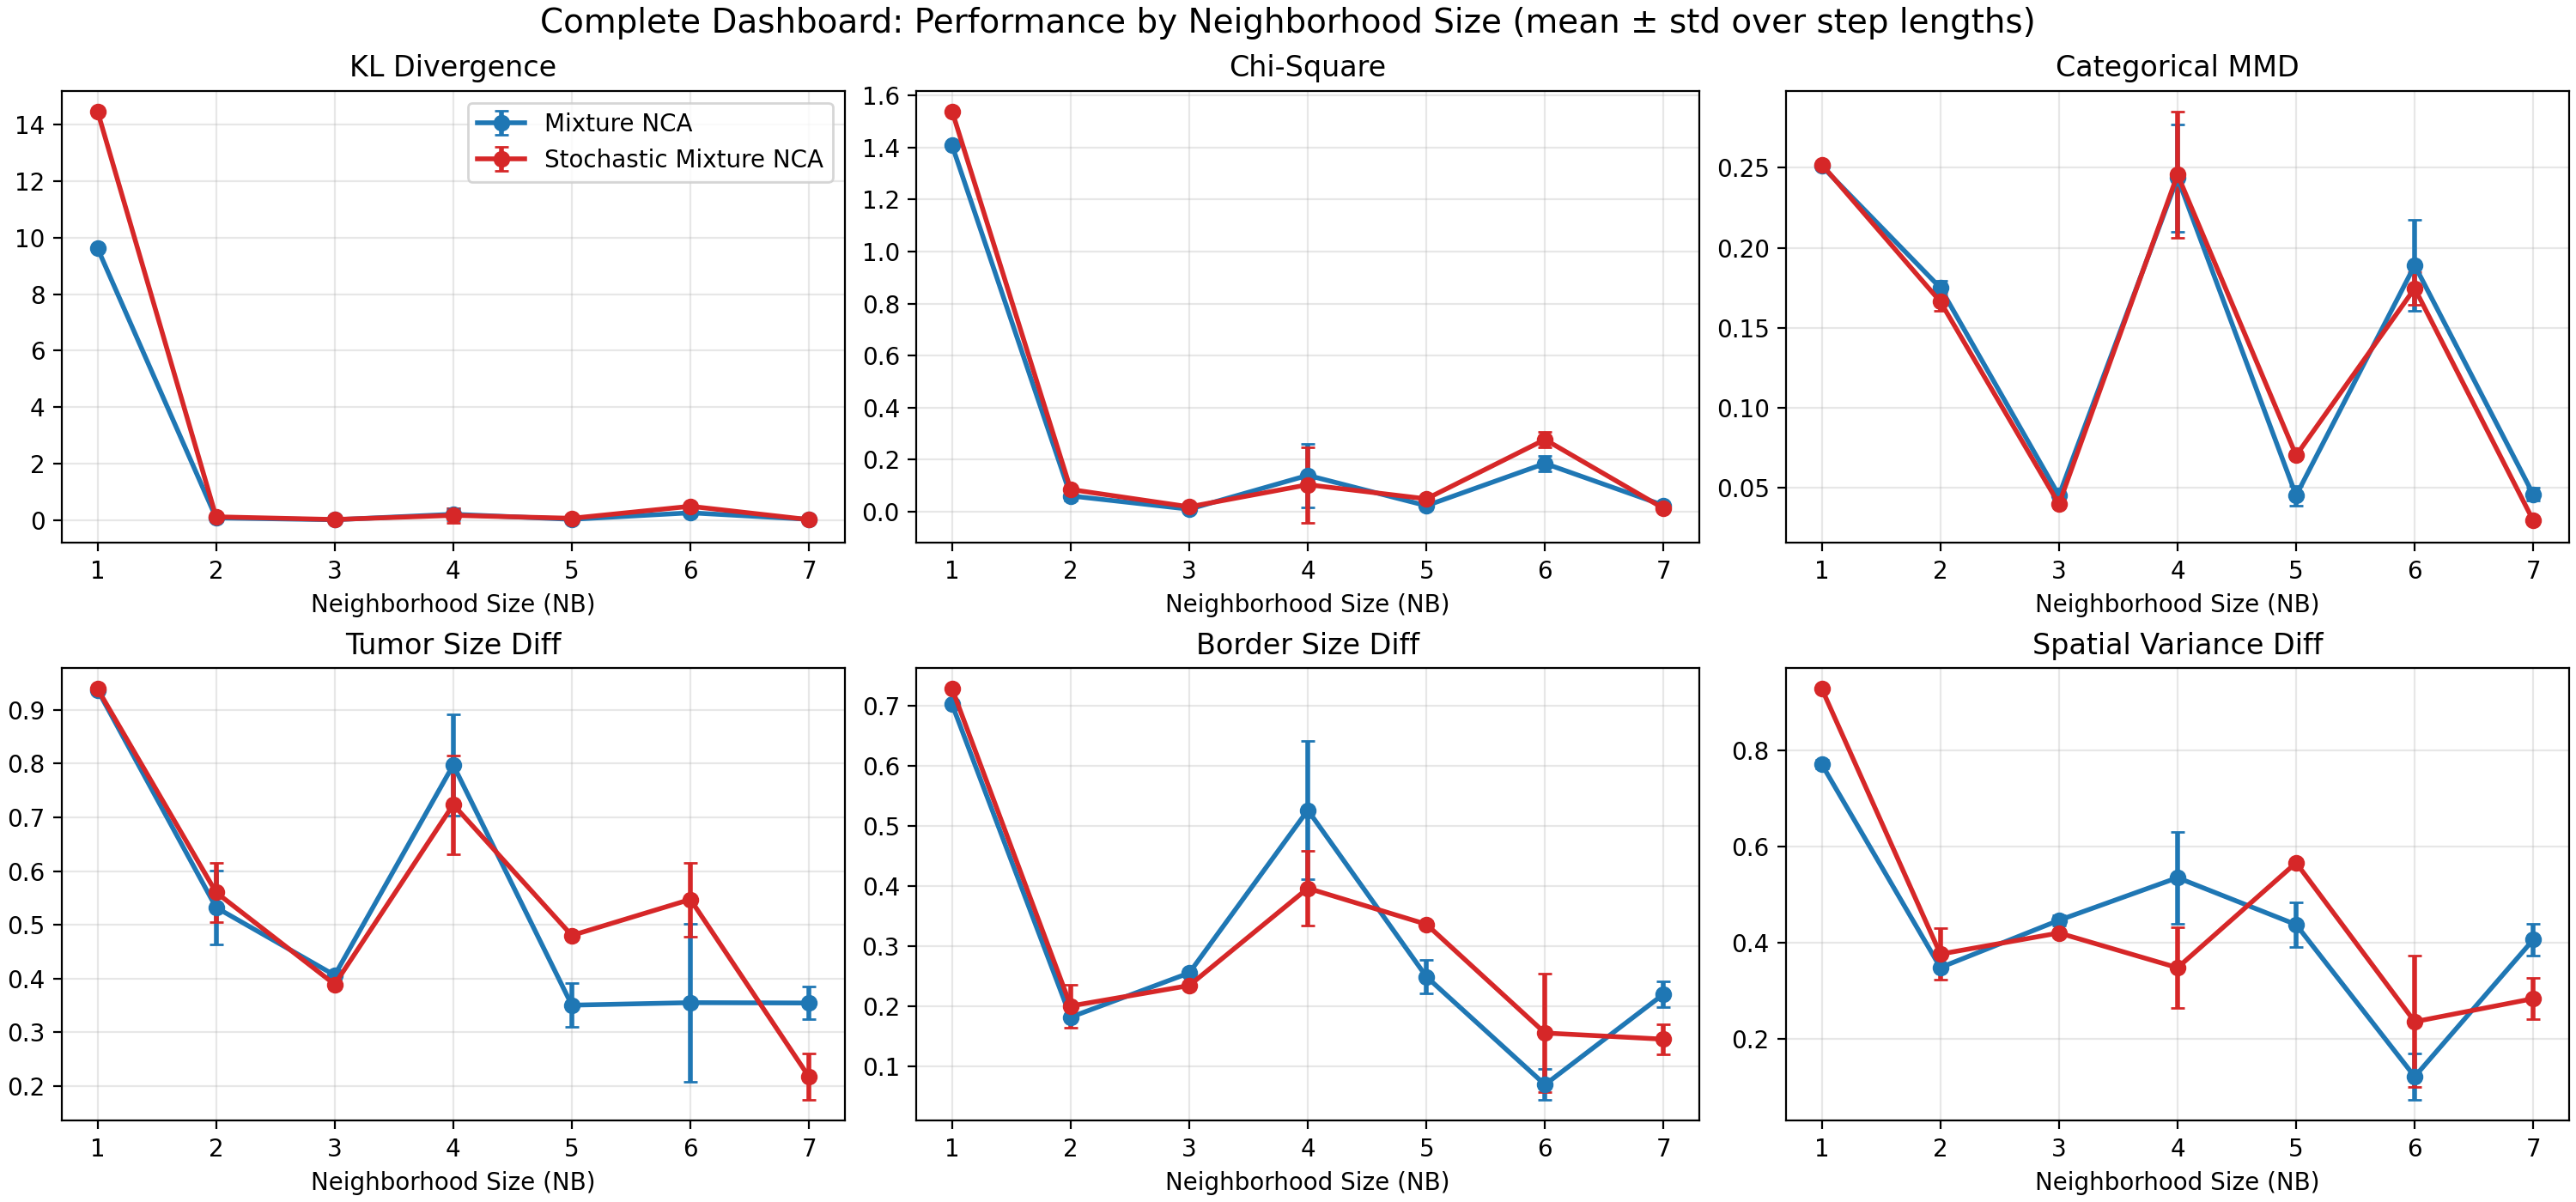
\includegraphics[width=\textwidth]{figs/neighborhood_analysis/nb_sweep_300x100/metrics_dashboard_full.png}
  \caption{Step 3: complete dashboard for the neighbourhood sweep. \textbf{Legend:} each panel is one of the six metrics (KL divergence, Chi-square, categorical MMD~\cite{gretton2012mmd}, tumour size difference, border size difference, spatial variance difference); abscissa = neighbourhood size \(NB\); ordinate = metric value (lower is better); mean and standard deviation over step-length conditions; series distinguish Mixture NCA vs.\ Stochastic Mixture NCA.}
  \label{fig:impl:step3:dashboard}
\end{figure}

\newpage
\vspace{-0.5em}
\subsubsection{Distributional agreement and per-simulation variability}
\label{sec:results:step3:kl}
\vspace{-0.8em}
KL divergence captures how well the global composition of cell types in the generated final state matches the empirical distribution from the dataset.
Across all step lengths, \(NB=1\) yields very large KL values, indicating a strong mismatch in global composition.
For \(NB\ge2\), both models reach low KL on average, but the best neighbourhood can depend on the evaluation horizon and on whether rule selection is deterministic or stochastic.
\vspace{-0.4em}
To interpret robustness, we inspect \emph{per-simulation} distributions of the metrics using violin plots.
Compared to mean-only summaries, violins reveal heavy tails and outliers: these correspond to runs that converge to qualitatively wrong outcomes (failure modes), even when the median performance is competitive.
\vspace{-0.6em}
\begin{figure}[H]
  \centering
  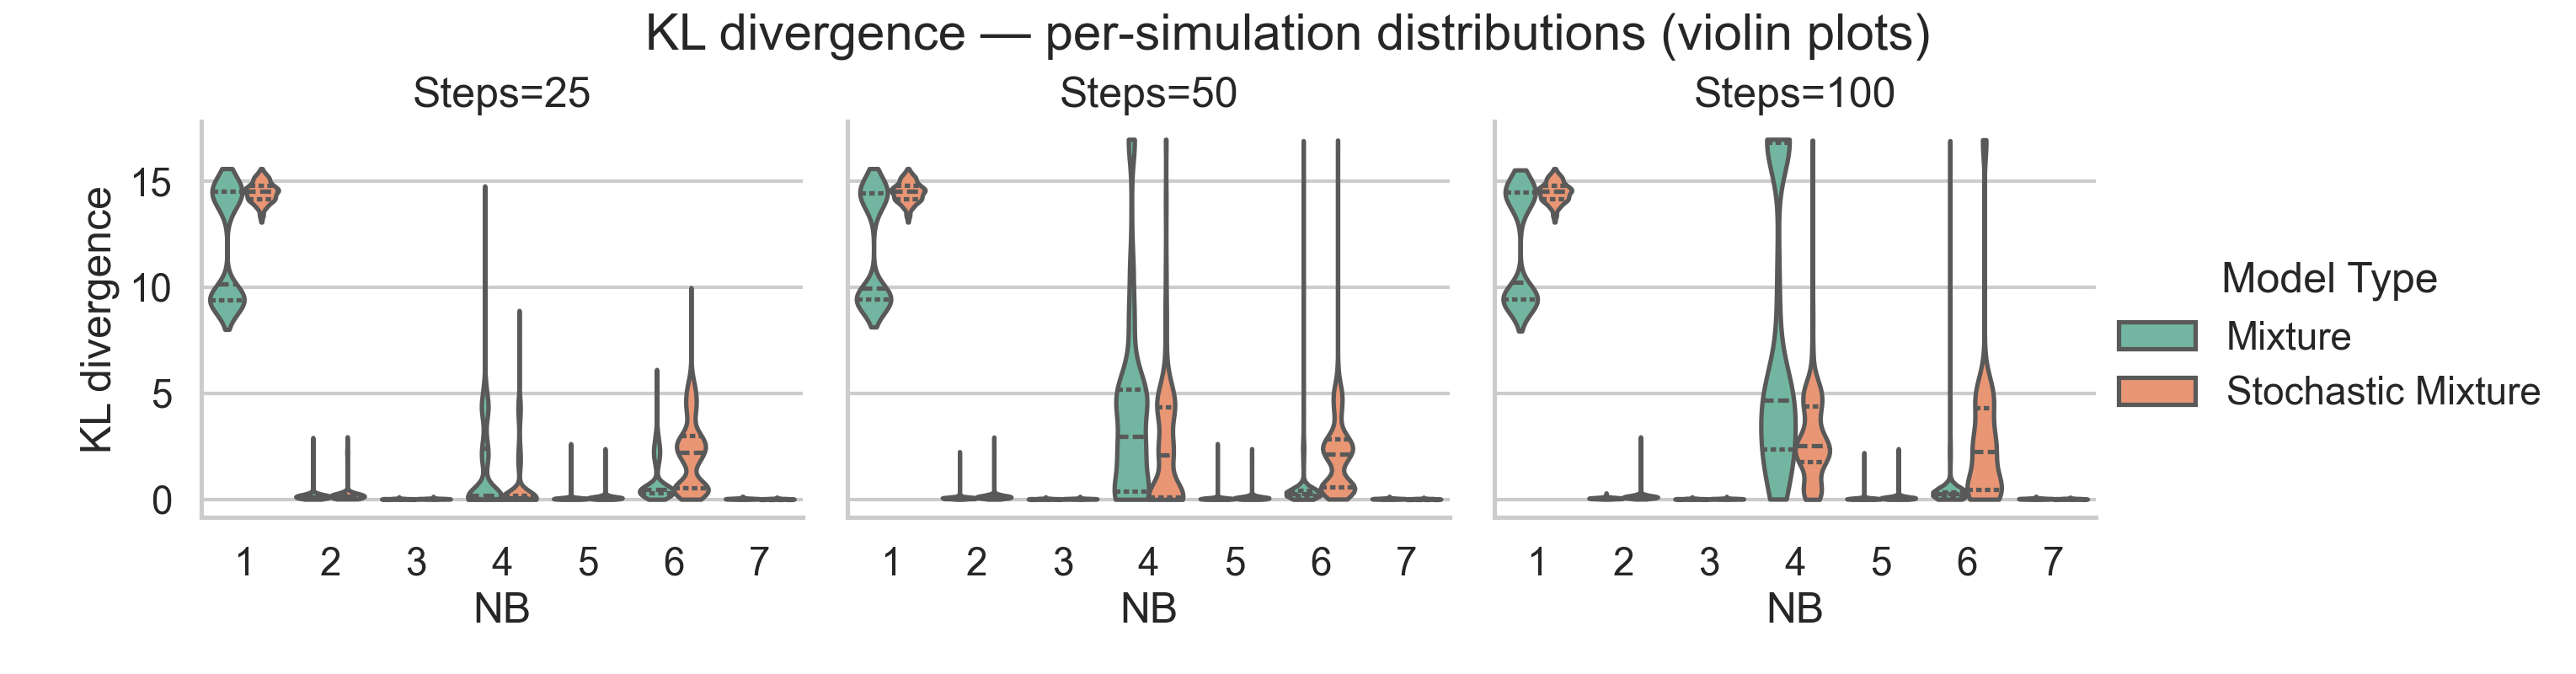
\includegraphics[width=\textwidth]{figs/neighborhood_analysis/nb_sweep_300x100/violin_KL_Divergence.png}
  \caption{Step 3: per-simulation violin plots for KL divergence. \textbf{Legend:} abscissa = neighbourhood size \(NB\); ordinate = KL divergence (lower is better); one violin per \((NB,\text{model})\); columns = step length (25, 50, 100); violin width = density of runs; inner line = quartiles.}
  \label{fig:impl:step3:violin:kl}
\end{figure}
\vspace{-0.5em}
\newpage

\begin{figure}[H]
  \centering
  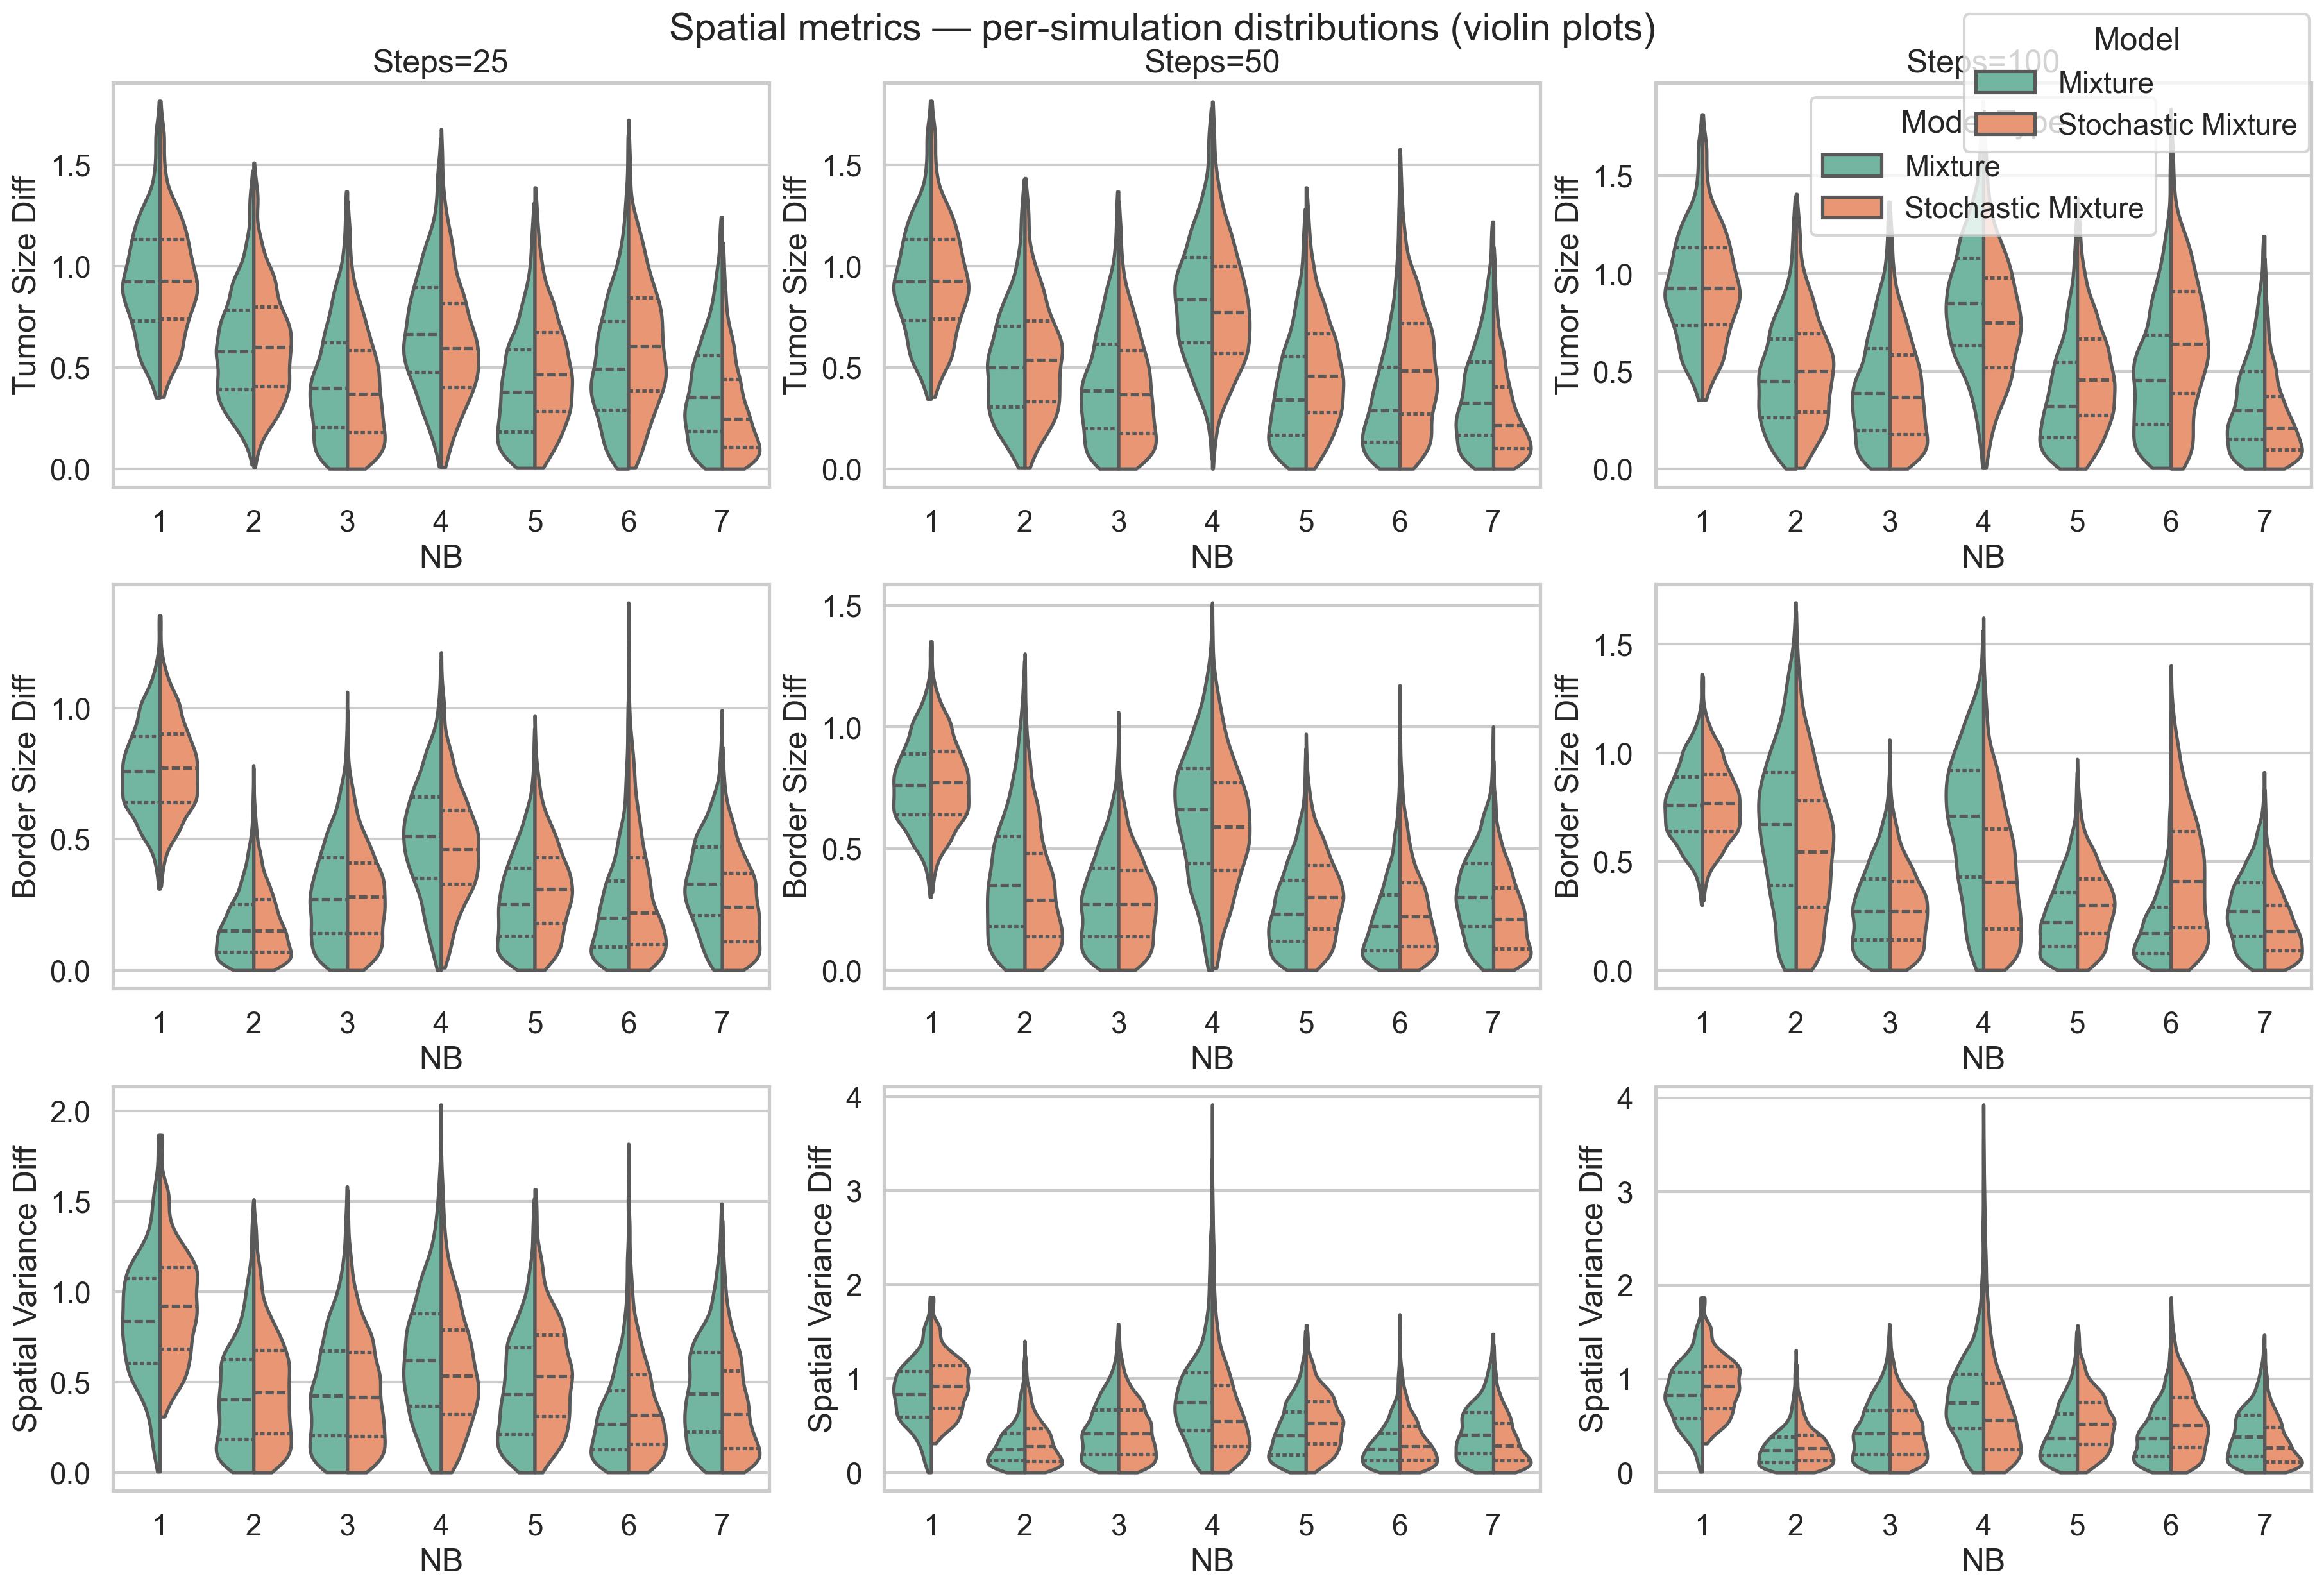
\includegraphics[width=\textwidth]{figs/neighborhood_analysis/nb_sweep_300x100/violin_spatial_metrics.png}
  \caption{Step 3: per-simulation violin plots for spatial metrics. \textbf{Legend:} three panels (tumour size difference, border size difference, spatial variance difference); abscissa = \(NB\); ordinate = metric value (lower is better); columns = step length; violin width = density, inner line = quartiles; series = Mixture vs.\ Stochastic Mixture NCA.}
  \label{fig:impl:step3:violin:spatial}
\end{figure}

\subsubsection{A dynamical bias--variance lens}
\label{sec:results:step3:biasvariance}
Although our setting is not classical supervised learning, the observed patterns can be interpreted through a \emph{structural and dynamical} bias--variance lens.
Here, \emph{bias} refers to systematic mismatch of the generated dynamics across simulations (persistently large mean errors), while \emph{variance} refers to sensitivity to stochastic fluctuations and failure modes (dispersion, heavy tails, and occasional large deviations in per-simulation distributions).
Under this view, \(NB=1\) corresponds to a high-bias regime: multiple metrics exhibit consistently large discrepancies, indicating that the receptive field is too limited to represent the relevant spatial couplings.
Moving to \(NB\in\{2,3\}\) reduces this structural bias sharply (Figure~\ref{fig:impl:step3:dashboard}) and often yields more concentrated per-simulation distributions (Figures~\ref{fig:impl:step3:violin:kl} and \ref{fig:impl:step3:violin:spatial}), although robustness remains metric-dependent (e.g.\ KL can still show substantial tail risk relative to the best configuration at a given horizon).
At intermediate neighbourhoods (notably around \(NB=4\), and for KL also \(NB=6\)), the mean performance can remain competitive while tail behaviour worsens (heavy tails and elevated bad-rate), i.e.\ a higher-variance regime in a dynamical sense.
For some metrics and horizons, larger neighbourhoods (especially \(NB=7\)) reduce tail risk again, consistent with stronger spatial averaging and more stable long-horizon rollouts; however, the overall picture remains non-monotonic and metric-specific, and in some spatial metrics \(NB=6\) can be preferable in mean even when KL robustness favors \(NB=7\).
Finally, these variance effects become more pronounced at longer rollout horizons, supporting the interpretation that neighbourhood size changes the \emph{dynamical regime} and that instability can be amplified over time rather than appearing immediately.

\subsubsection{Trend analysis and fold change}
\label{sec:results:step3:trend}

To summarise how performance changes with neighbourhood size in a compact way, we also compute a simple trend analysis over \(NB\).
In particular, we report fold change between a reference neighbourhood (here \(NB=3\), used as a normalization point in the sweep) and a larger neighbourhood (here \(NB=7\)).
On the plot, values below 1 indicate improvement when increasing neighbourhood size from 3 to 7, while values above 1 indicate degradation; the interpretation depends on the metric and on the rollout horizon.
This is useful because in several metrics the main effect is the jump from \(NB=1\) to \(NB\ge2\), while differences among \(NB\ge2\) are smaller and may depend on the metric.

\begin{figure}[H]
  \centering
  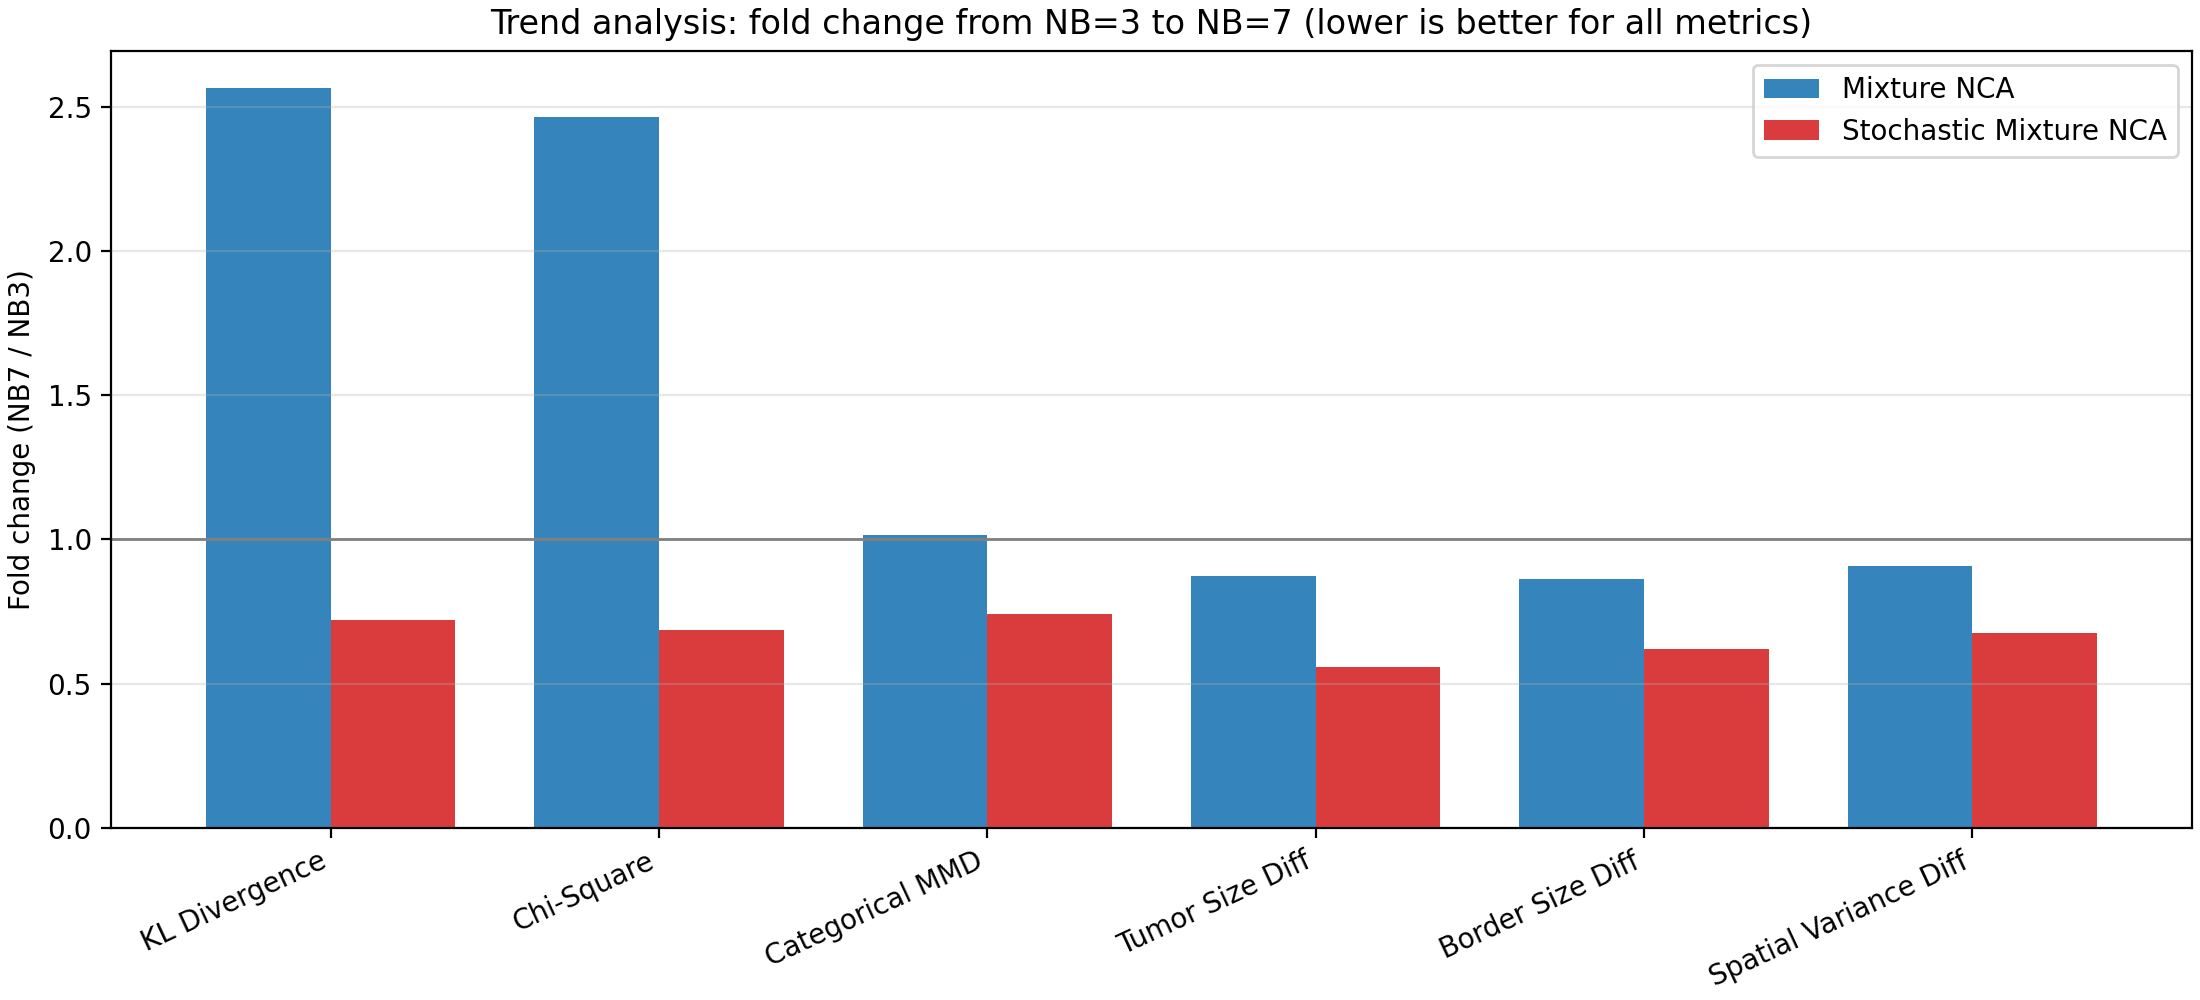
\includegraphics[width=\textwidth]{figs/neighborhood_analysis/nb_sweep_300x100/trend_foldchange_nb7_over_nb3.png}
  \caption{Step 3: trend analysis via fold change from \(NB=3\) to \(NB=7\). \textbf{Legend:} ratio \(\mathrm{metric}(NB=7)/\mathrm{metric}(NB=3)\) on the ordinate (reference line at 1); abscissa = metric; panels by step length and model type.}
  \label{fig:impl:step3:trend:foldchange}
\end{figure}

\subsubsection{Robustness via bad-rate}
\label{sec:results:step3:badrate}

Mean values alone can hide important instability: per-simulation distributions often show heavy tails where a non-trivial fraction of runs ends in poor outcomes (``failure modes'').
To quantify this, we define a \emph{bad-rate} as follows: for each metric and each (model, step length), we select the neighbourhood size with the best median performance, take the 95th percentile of that best distribution as a threshold, and compute for each \(NB\) the probability that a run exceeds this threshold.

\begin{figure}[H]
  \centering
  
\includegraphics[width=\textwidth]{figs/neighborhood_analysis/nb_sweep_300x100/badrate_bars_KL_Divergence.png}
  \caption{Step 3: bad-rate for KL divergence. \textbf{Legend:} abscissa = \(NB\); ordinate = fraction of runs whose KL exceeds the 95th percentile of the best \(NB\) for that (model, step length); columns = step length; bars = Mixture vs.\ Stochastic Mixture NCA; lower is better.}
  \label{fig:impl:step3:badrate:kl}
\end{figure}

\begin{figure}[H]
  \centering
  
\includegraphics[width=\textwidth]{figs/neighborhood_analysis/nb_sweep_300x100/badrate_bars_Tumor_Size_Diff.png}
  \caption{Step 3: bad-rate for tumour size difference. \textbf{Legend:} same as Figure~\ref{fig:impl:step3:badrate:kl} (abscissa = \(NB\), ordinate = fraction of runs above threshold, columns = step length, series = model type; lower is better).}
  \label{fig:impl:step3:badrate:tumor}
\end{figure}

\begin{figure}[H]
  \centering
  
\includegraphics[width=\textwidth]{figs/neighborhood_analysis/nb_sweep_300x100/badrate_bars_Border_Size_Diff.png}
  \caption{Step 3: bad-rate for border size difference. \textbf{Legend:} same layout as Figure~\ref{fig:impl:step3:badrate:kl} (abscissa = \(NB\), ordinate = bad-rate fraction, columns = step length; lower is better).}
  \label{fig:impl:step3:badrate:border}
\end{figure}

\begin{figure}[H]
  \centering
  
\includegraphics[width=\textwidth]{figs/neighborhood_analysis/nb_sweep_300x100/badrate_bars_Spatial_Variance_Diff.png}
  \caption{Step 3: bad-rate for spatial variance difference. \textbf{Legend:} same layout as Figure~\ref{fig:impl:step3:badrate:kl} (abscissa = \(NB\), ordinate = bad-rate fraction, columns = step length; lower is better).}
  \label{fig:impl:step3:badrate:spvar}
\end{figure}

\subsubsection{Computational complexity and rule specialization}
\label{sec:results:step3:complexity_rules}

Figure~\ref{fig:impl:step3:complexity} reports the empirical runtime as a function of neighbourhood size.
In the explored range \(NB\in[1,7]\), the measured runtime remains approximately flat.
Empirically, Mixture NCA runs at about \(\sim 1.5\) ms/step on average, while the Stochastic Mixture variant is about \(\sim 3.2\) ms/step, with limited variation across neighbourhood size.
This suggests that in this implementation range the practical cost is dominated by constants and vectorization effects rather than by the naive theoretical \(O(NB^2)\) scaling.

\begin{figure}[H]
  \centering
  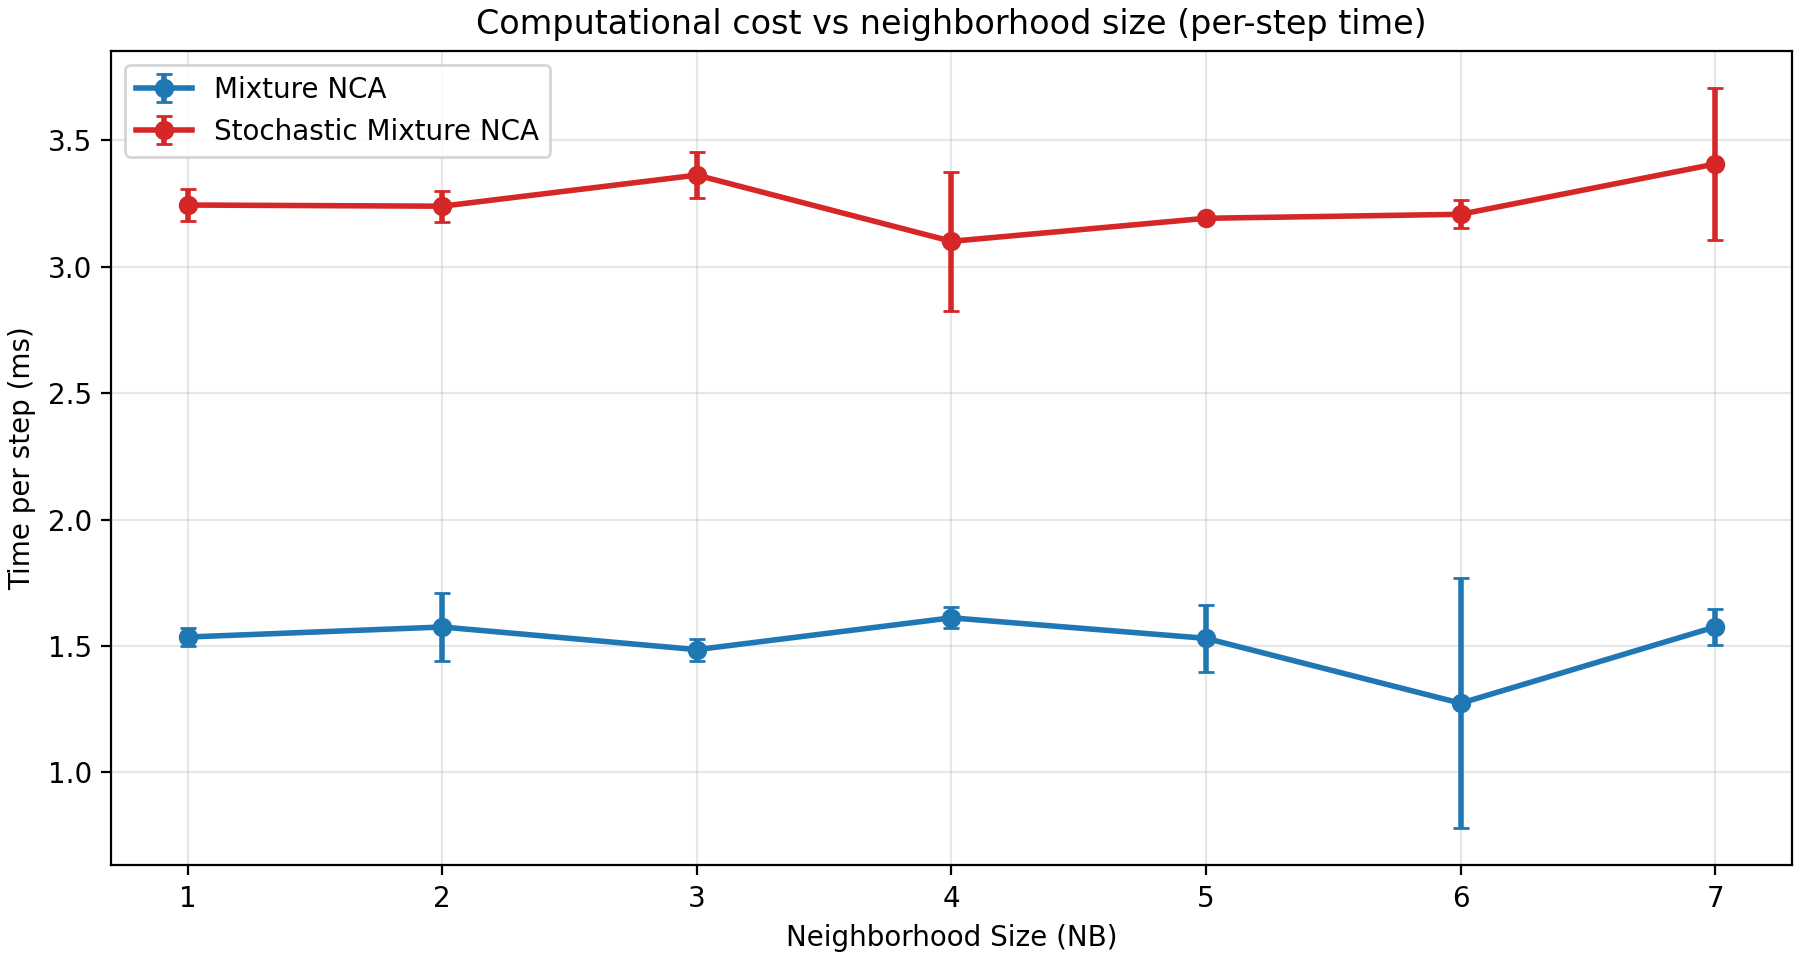
\includegraphics[width=0.85\textwidth]{figs/neighborhood_analysis/nb_sweep_300x100/computational_complexity_time_per_step.png}
  \caption{Step 3: empirical computational cost vs neighbourhood size. \textbf{Legend:} abscissa = \(NB\); ordinate = time per simulation step (ms); two series = Mixture NCA and Stochastic Mixture NCA; error bars = variability over repeated timing runs.}
  \label{fig:impl:step3:complexity}
\end{figure}

\begin{figure}[H]
  \centering
  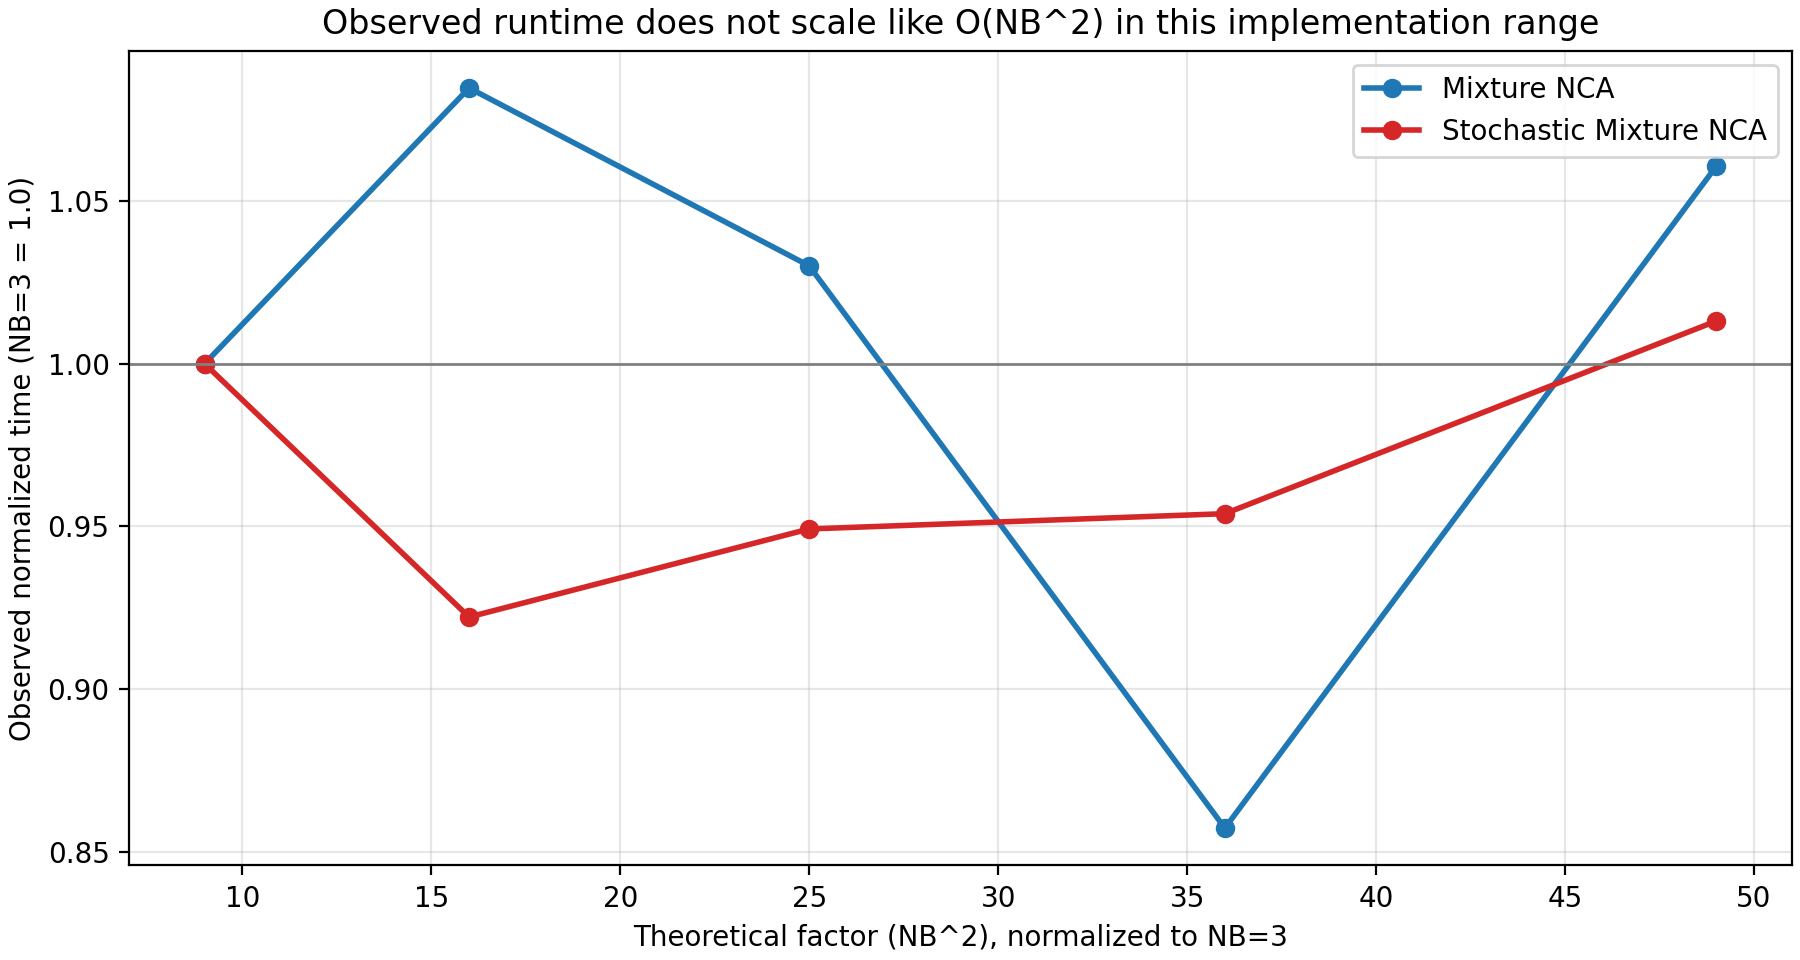
\includegraphics[width=0.85\textwidth]{figs/neighborhood_analysis/nb_sweep_300x100/computational_complexity_normalized_vs_theory.png}
  \caption{Step 3: normalized runtime vs.\ \(NB\). \textbf{Legend:} abscissa = \(NB\); ordinate = time relative to \(NB=3\) (value 1.0 = same as \(NB=3\)); series = Mixture vs.\ Stochastic Mixture NCA.}
  \label{fig:impl:step3:complexity:theory}
\end{figure}

Finally, we analyze how rules are selected over time as a function of neighbourhood size, which provides a qualitative explanation for the observed trade-offs and stability differences.
To study how specialization evolves during the dynamics, we measure the entropy of the model's rule-assignment distribution \(p(r \mid x_t)\) at each time step, averaged over space and over sampled simulations.
Low entropy indicates confident (specialized) rule selection, while higher entropy indicates mixed or uncertain rule usage.

\begin{figure}[H]
  \centering
  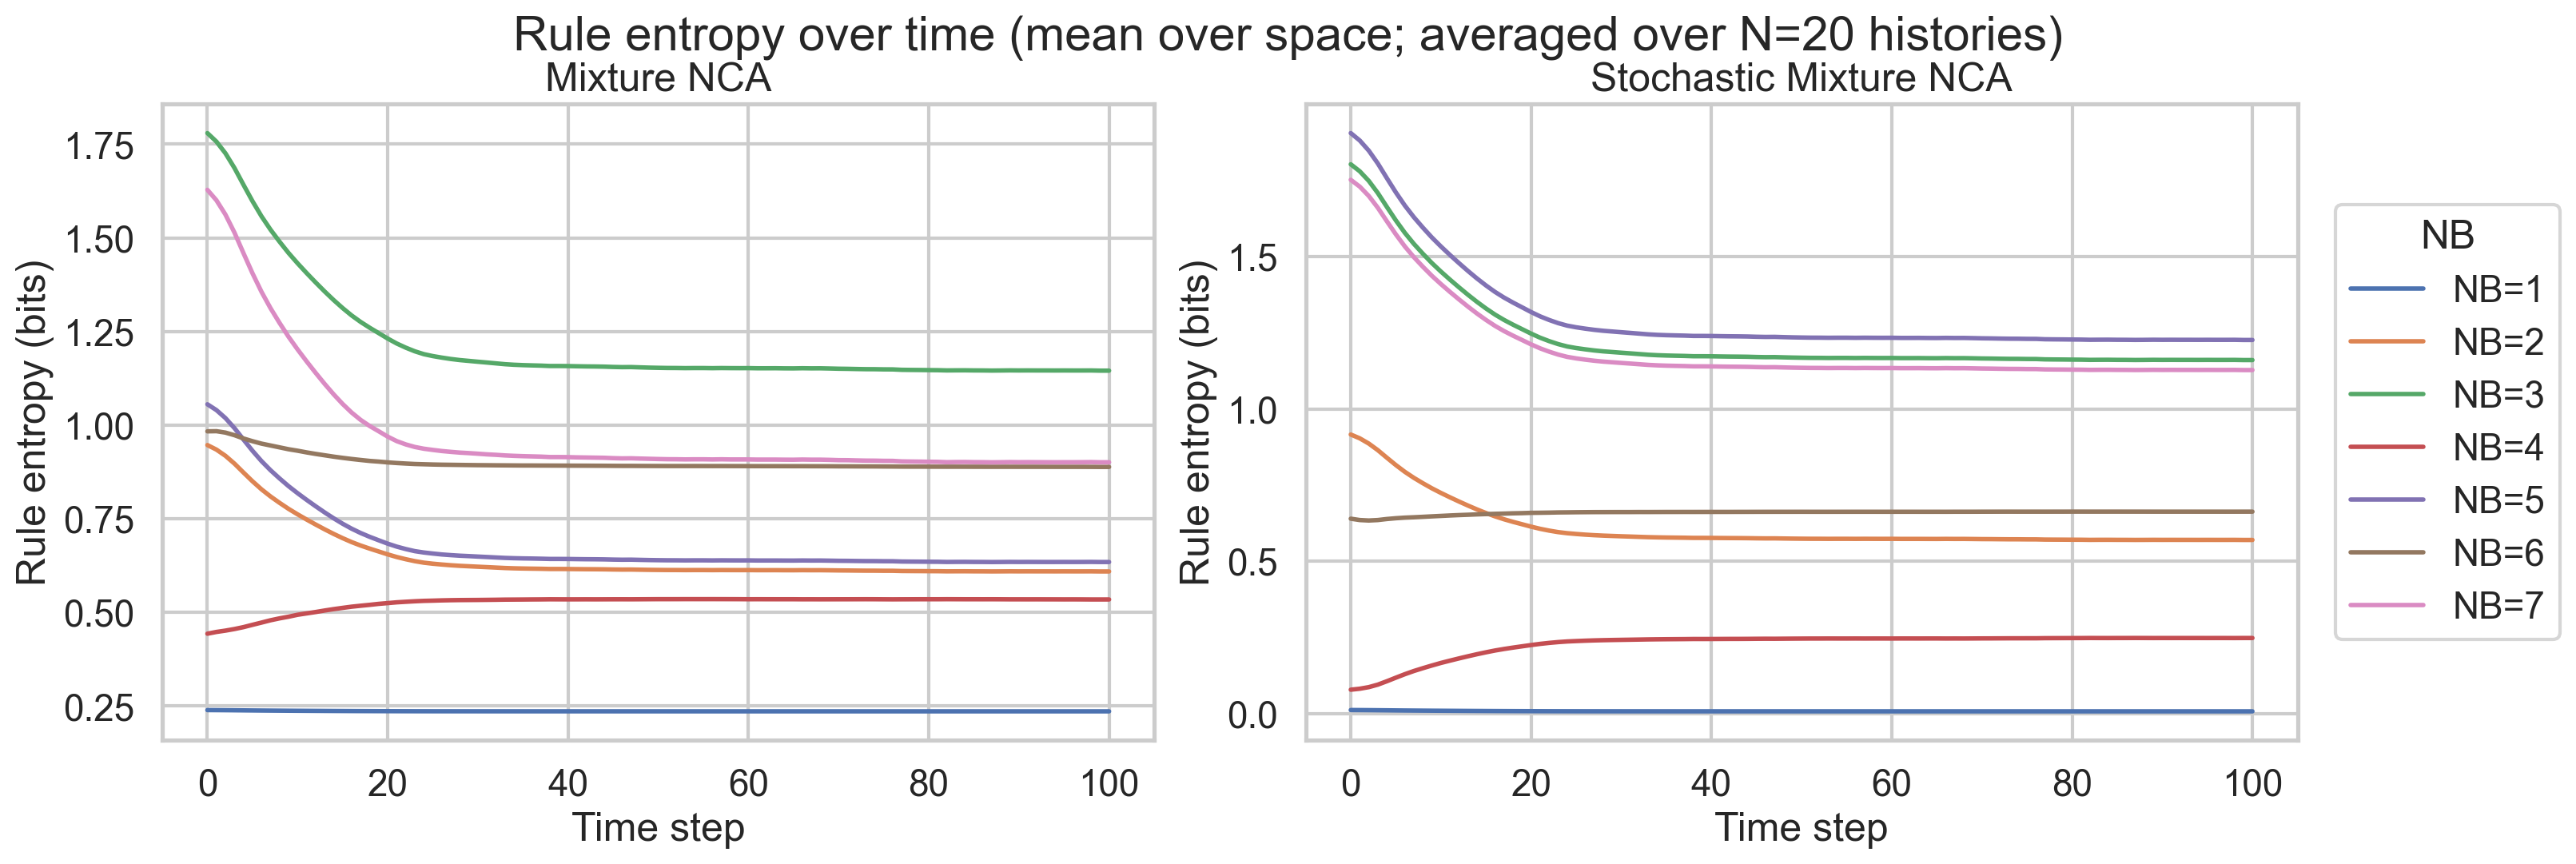
\includegraphics[width=\textwidth]{figs/neighborhood_analysis/nb_sweep_300x100/rule_entropy_over_time.png}
  \caption{Step 3: rule-assignment entropy over time. \textbf{Legend:} abscissa = simulation step; ordinate = entropy (bits), averaged over space and over \(N=20\) histories; one curve per neighbourhood size \(NB\); left panel = Mixture NCA, right panel = Stochastic Mixture NCA.}
  \label{fig:impl:step3:entropy:time}
\end{figure}

To complement the time-series view, we also summarize rule specialization with three simple indicators:
\begin{itemize}
  \item mean entropy (lower means more confident selection),
  \item rule diversity (higher means probability mass is spread over more rules),
  \item max rule usage (the maximum average probability assigned to a single rule; lower means more balanced usage).
\end{itemize}
Figure~\ref{fig:impl:step3:rule:summary} reports these indicators and relates them to KL divergence at Step Length \(=100\).
The resulting scatter does \emph{not} support a simple inverse (or linear) relation between specialization and dynamic divergence once \(NB\ge2\).
KL divergence is large mainly in the strongly constrained regime (\(NB=1\)): the model can commit confidently (low entropy) while still producing a large distributional mismatch, because it lacks spatial context and the resulting dynamics drift toward wrong global compositions.
For \(NB\ge2\), configurations with higher entropy (more mixed rule usage) can achieve equally low or even lower KL than more specialized ones, suggesting that mescolanza can be compatible with (and in some cases associated with) more stable long-horizon dynamics.
Therefore, rule specialization should be treated as a diagnostic of the operating regime (constraint vs.\ flexibility) rather than as a direct predictor of distributional fidelity.

\begin{figure}[H]
  \centering
  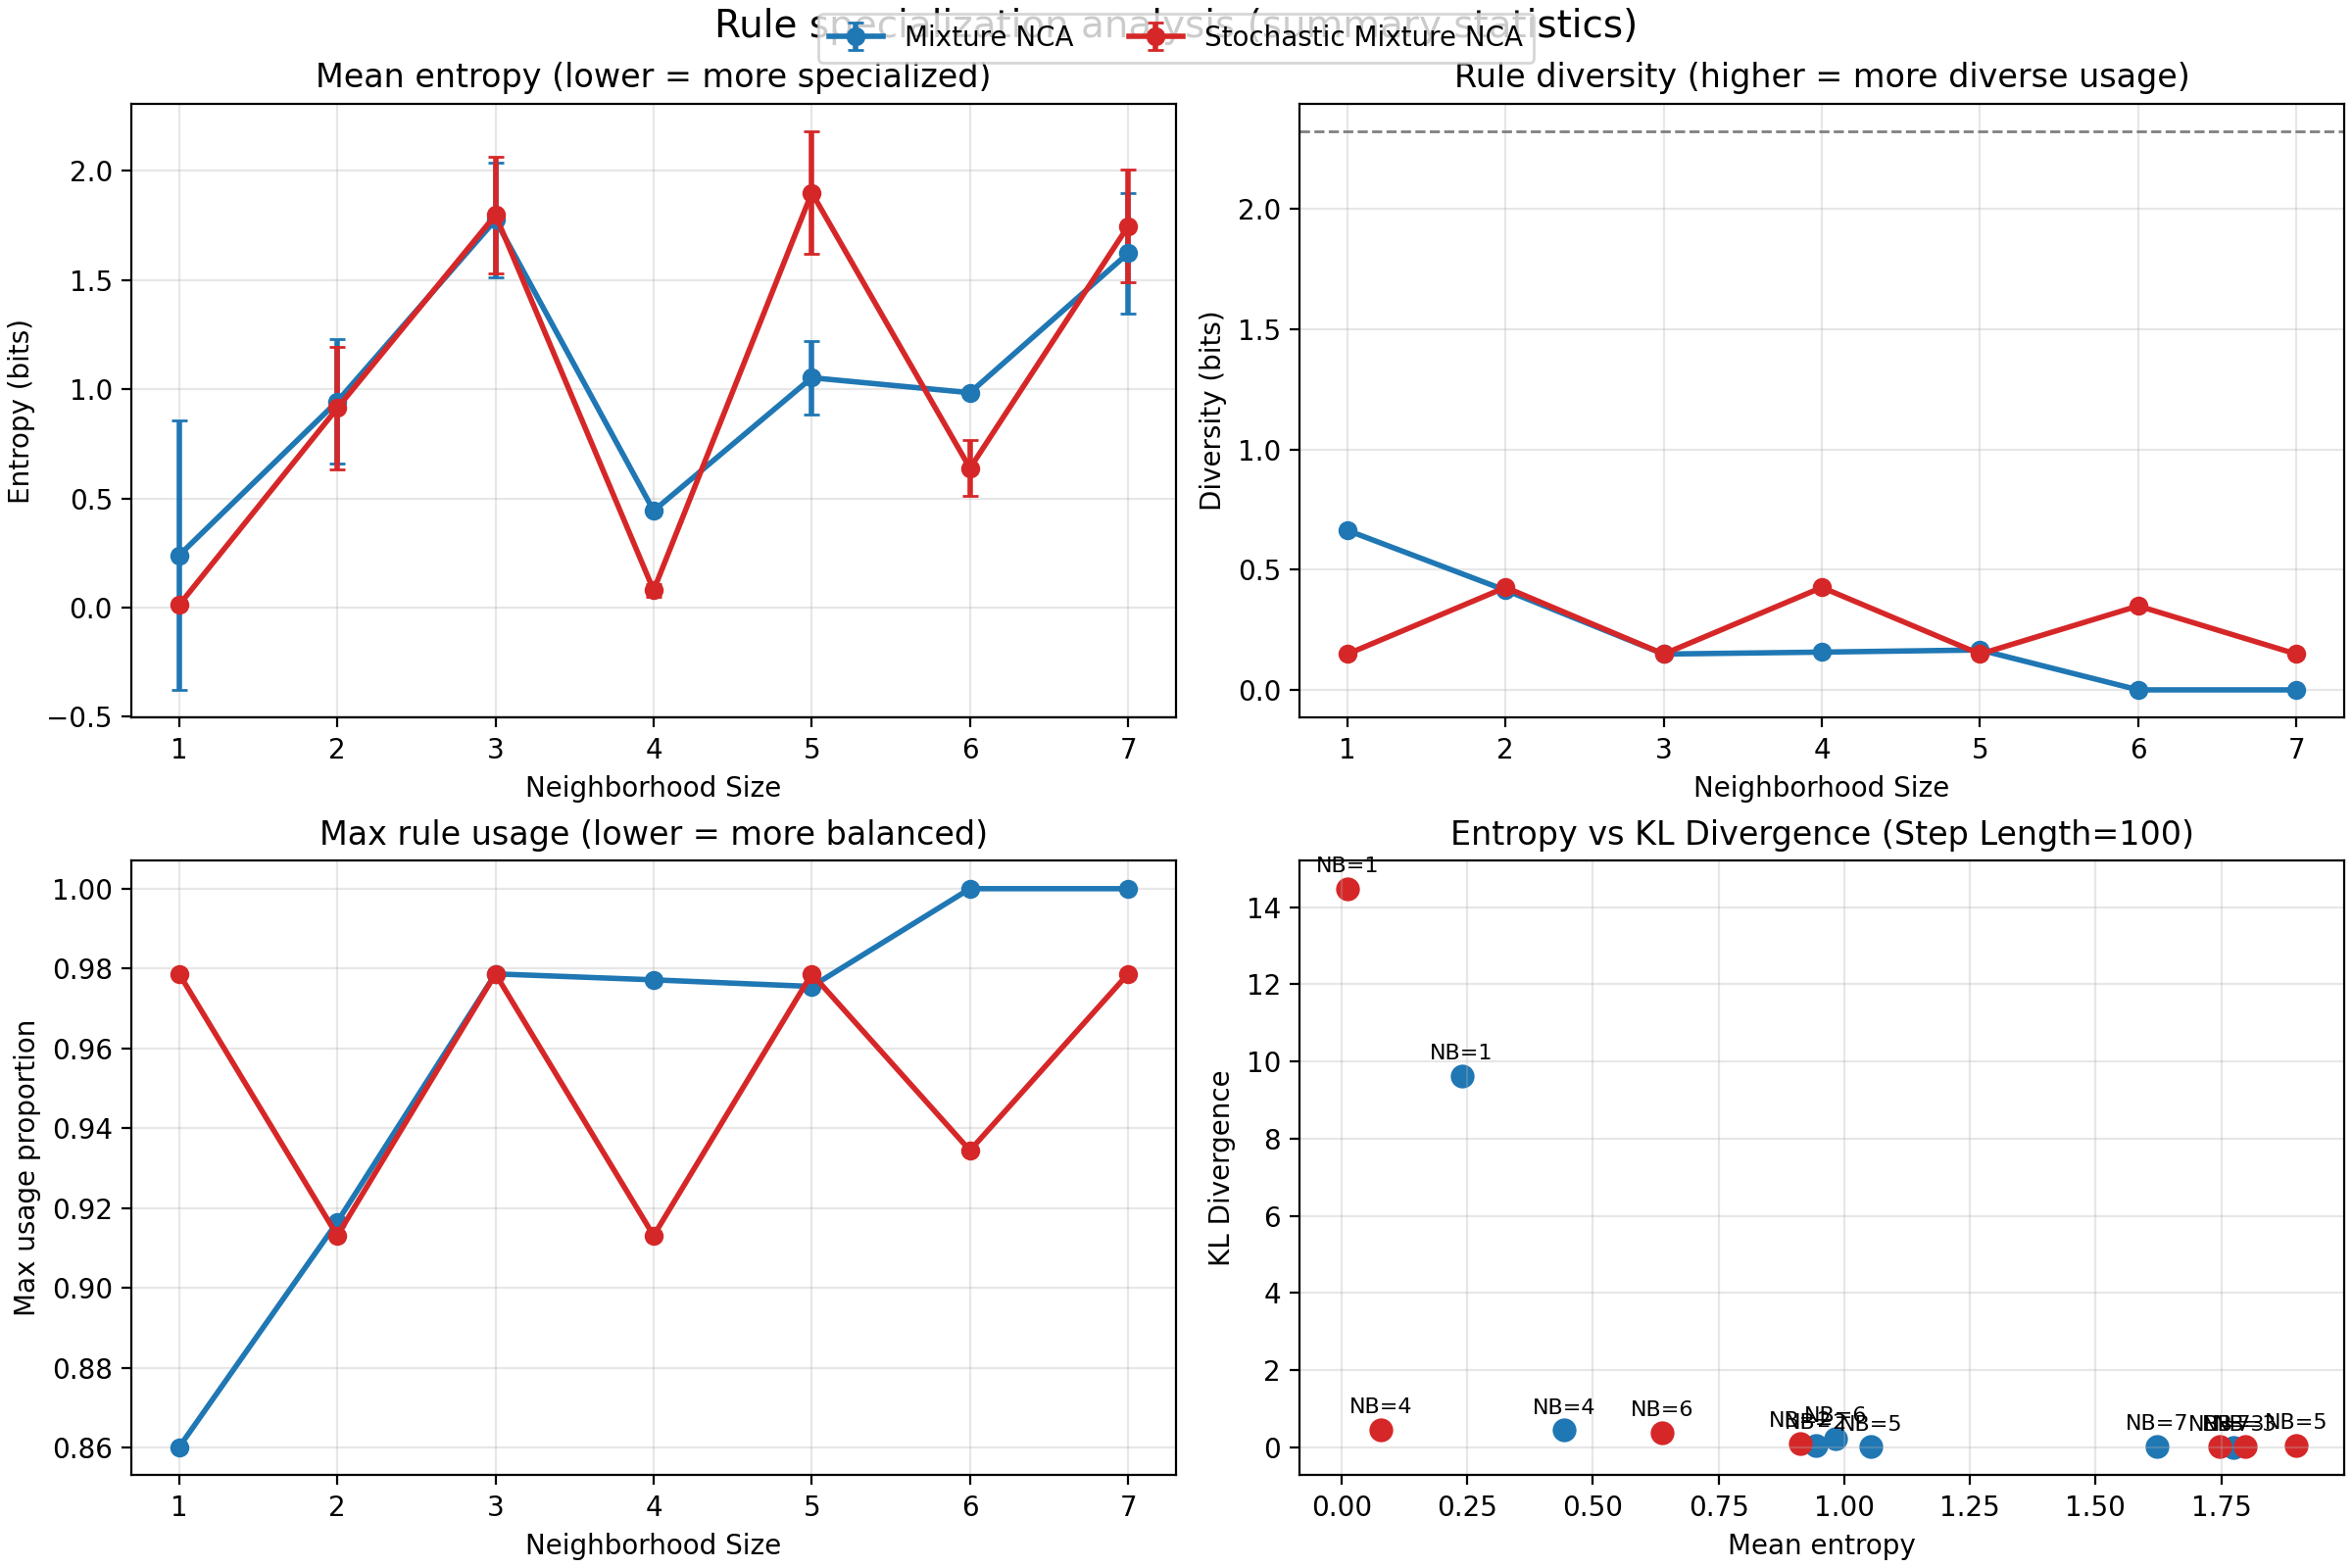
\includegraphics[width=\textwidth]{figs/neighborhood_analysis/nb_sweep_300x100/rule_specialization_summary.png}
  \caption{Step 3: rule specialization summary. \textbf{Legend:} four panels (mean entropy, rule diversity, max rule share, and scatter entropy vs.\ KL at step length 100); points/series = neighbourhood sizes \(NB\); bottom-right panel: abscissa = entropy, ordinate = KL divergence at step length 100.}
  \label{fig:impl:step3:rule:summary}
\end{figure}

\newpage
To make rule selection more intuitive, we also visualize the \emph{rule-assignment probability maps} \(p(r \mid x)\) for a single example state.
Each heatmap shows, for each spatial position, how likely the model is to select a given rule, and the rows compare selected neighbourhood sizes.

\begin{figure}[H]
  \centering
  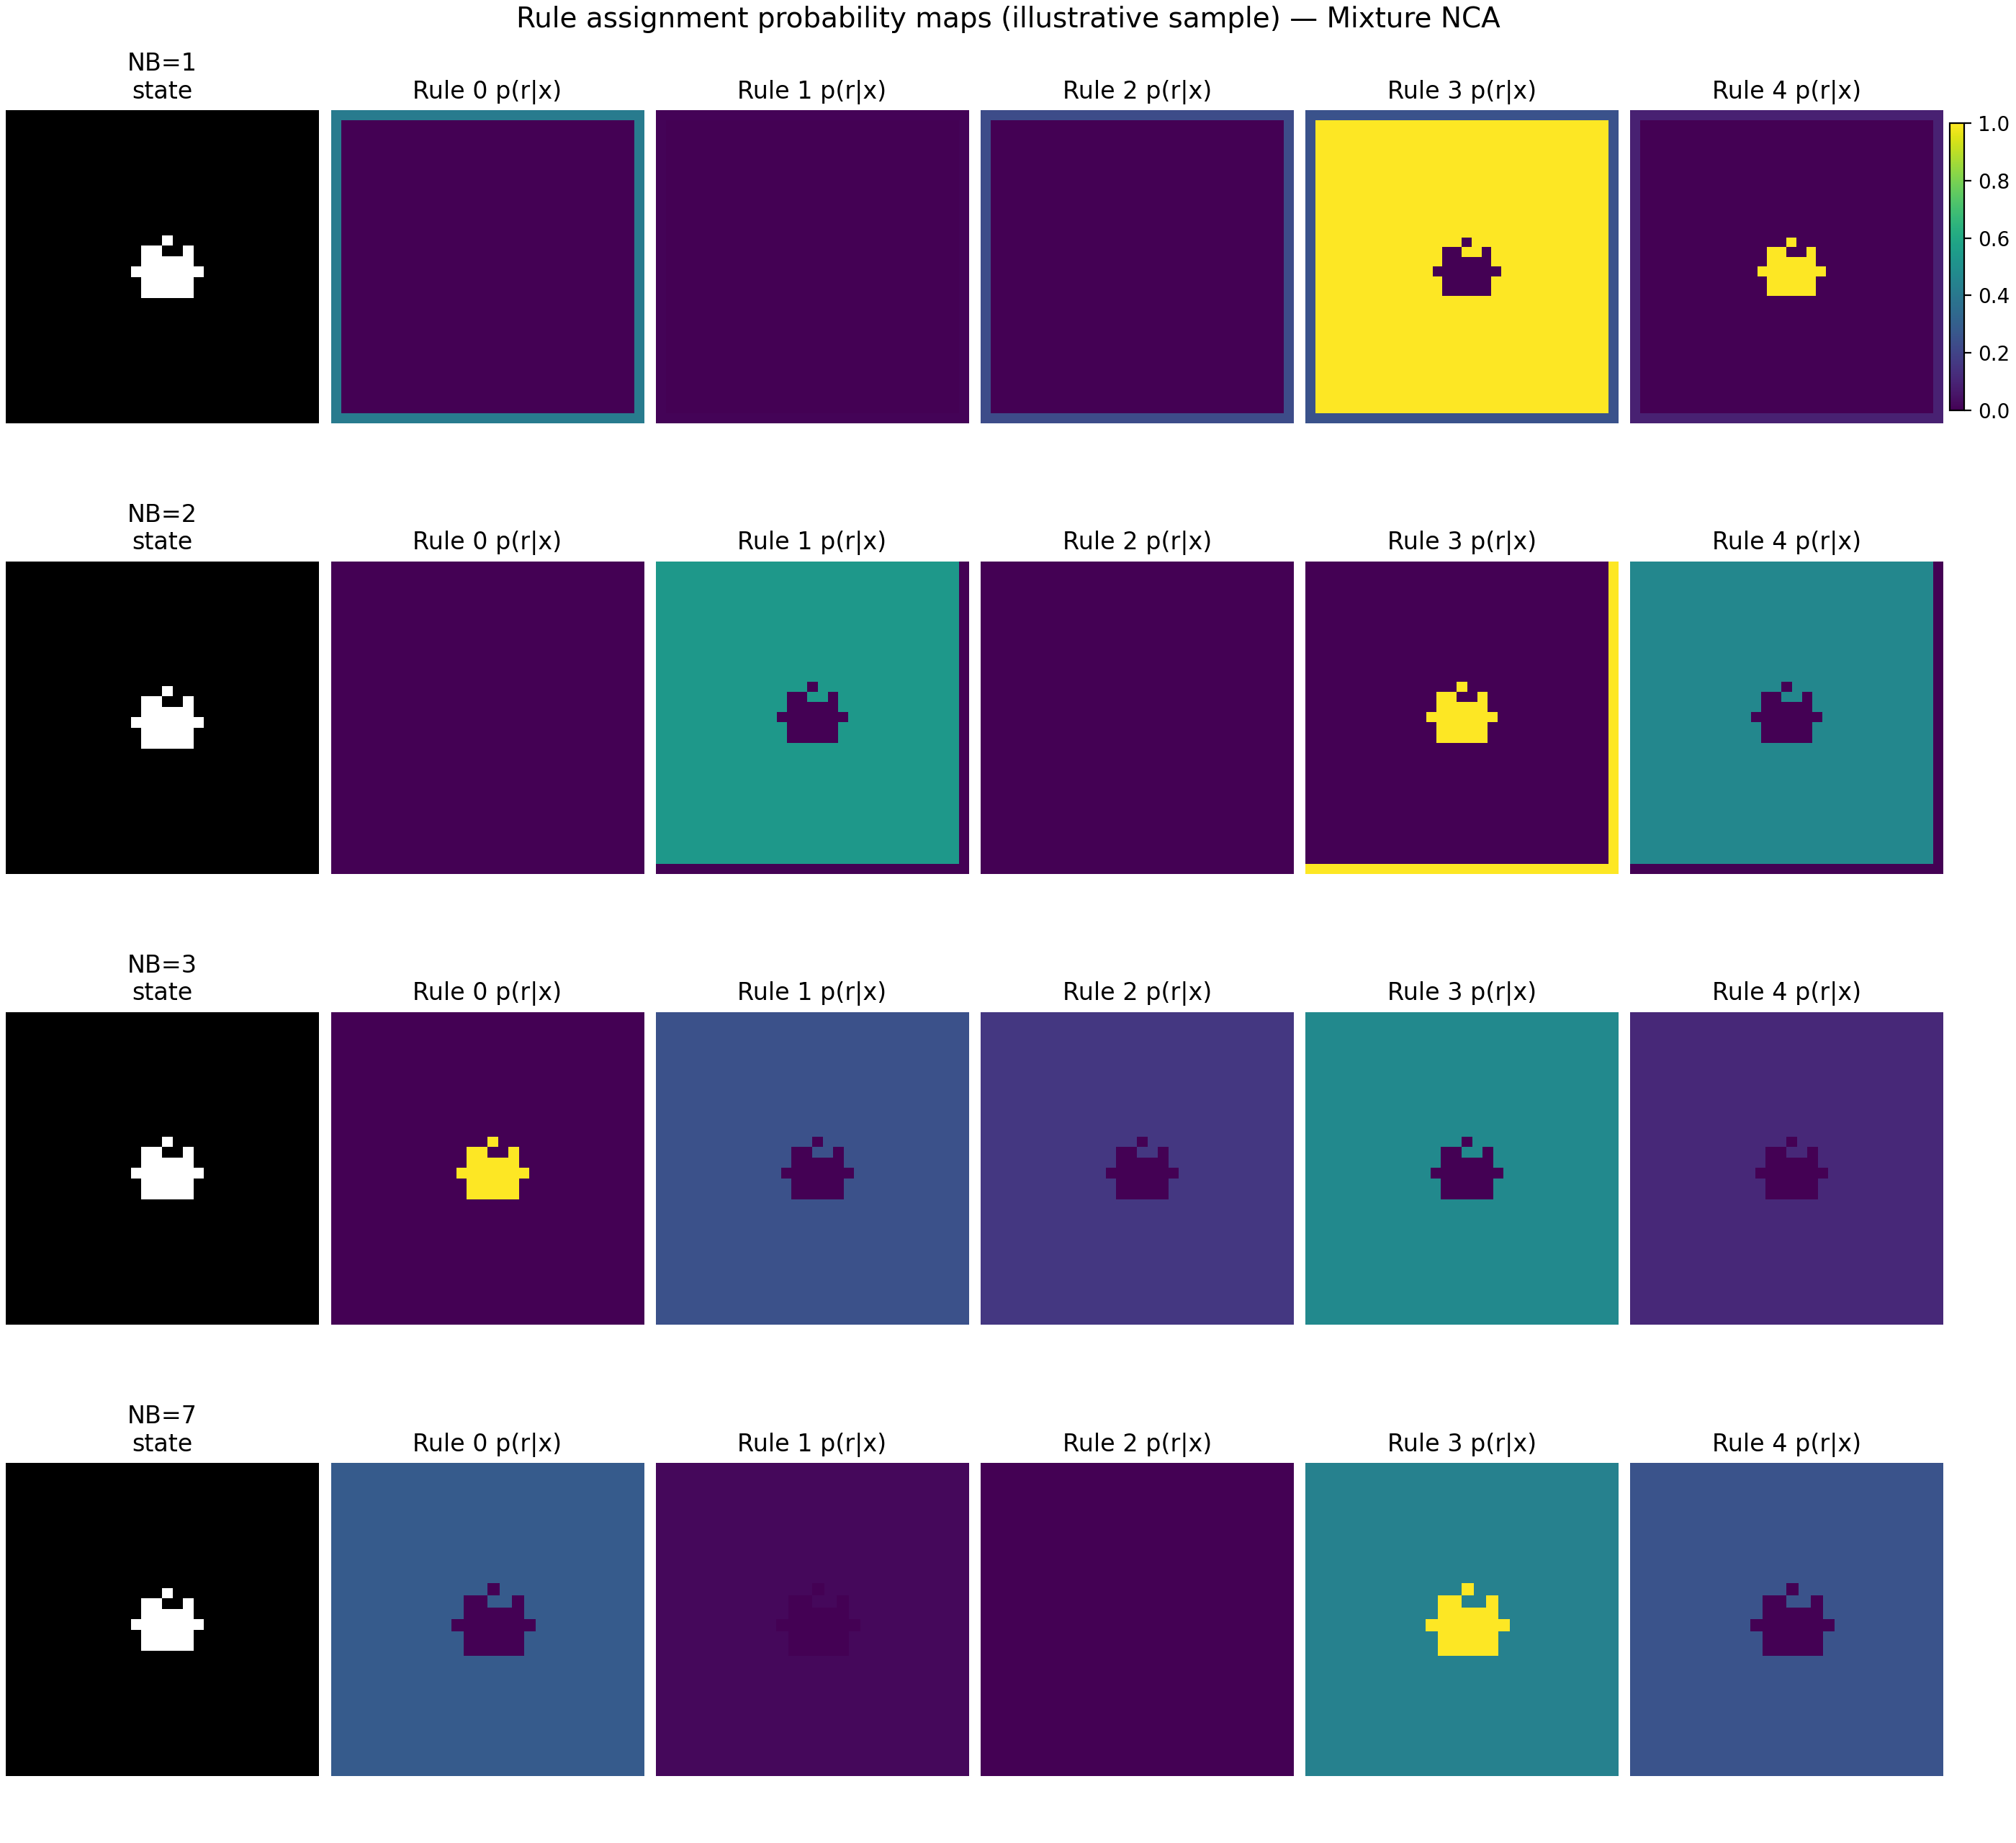
\includegraphics[width=\textwidth]{figs/neighborhood_analysis/nb_sweep_300x100/rule_assignment_maps_mixture.png}
  \caption{Step 3: rule assignment probability maps for Mixture NCA (one example state). \textbf{Legend:} columns = input state and probability map for each of the five rules; rows = neighbourhood size \(NB\); colour intensity = probability of selecting that rule at each cell.}
  \label{fig:impl:step3:rule:maps:mix}
\end{figure}

\begin{figure}[H]
  \centering
  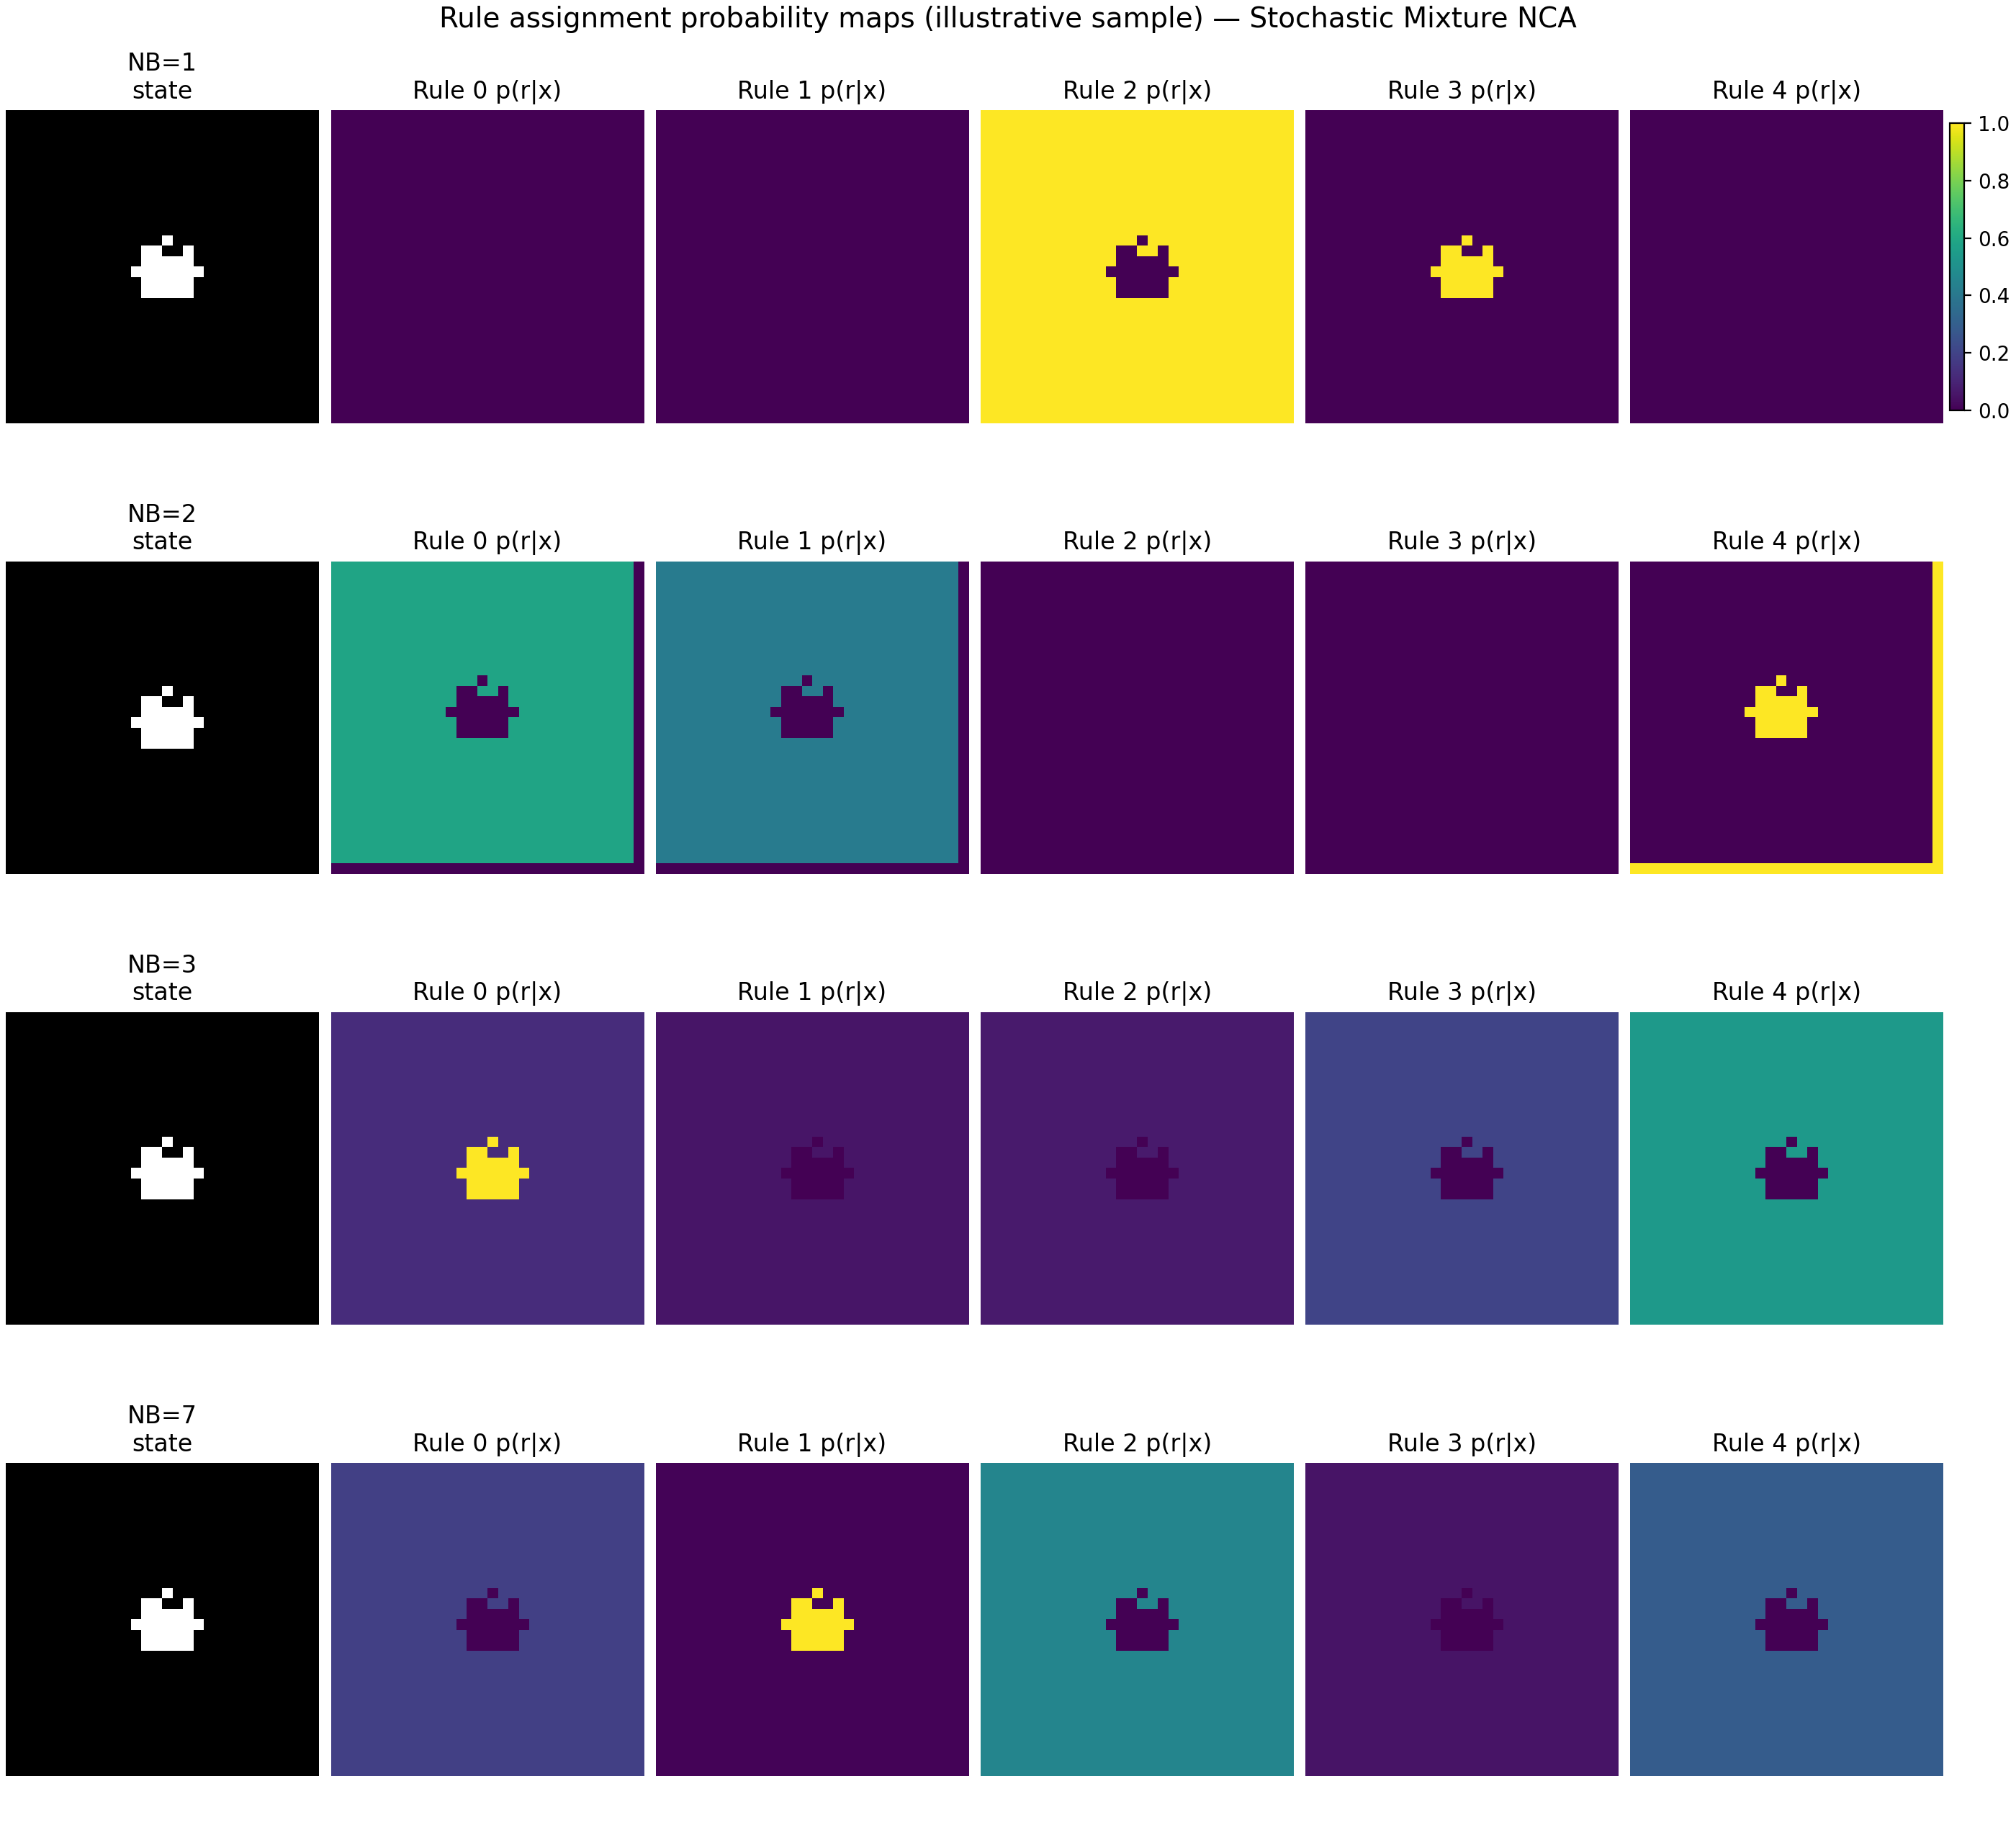
\includegraphics[width=\textwidth]{figs/neighborhood_analysis/nb_sweep_300x100/rule_assignment_maps_stochastic.png}
  \caption{Step 3: rule assignment probability maps for Stochastic Mixture NCA (one example state). \textbf{Legend:} same layout as Figure~\ref{fig:impl:step3:rule:maps:mix} (columns = state + five rule maps, rows = \(NB\); colour = probability).}
  \label{fig:impl:step3:rule:maps:stoch}
\end{figure}

\subsubsection{Statistical tests across neighbourhood sizes}
\label{sec:results:step3:stats}

% Auto-generated by experiments/generate_step3_stats_table.py
% Statistical tests: Step Length=100, baselines NB=2 and NB=3, Holm correction.
\begin{table}[H]
\centering
\small
\begin{tabulary}{\textwidth}{lLrLL}
\toprule
Model & Metric & Kruskal-Wallis $p$ & Significant vs NB=2 & Significant vs NB=3 \\
\midrule
Mixture~NCA & KL Divergence & $<10^{-4}$ & 3,4,5,6,7 & 4,5,6,7 \\
Mixture~NCA & Chi-Square & $<10^{-4}$ & 3,4,5,6,7 & 4,5,6,7 \\
Mixture~NCA & Categorical MMD & $<10^{-4}$ & 3,4,5,6,7 & 4,5,6 \\
Mixture~NCA & Tumour Size Diff & $<10^{-4}$ & 3,4,5,6,7 & 4,5,6,7 \\
Mixture~NCA & Border Size Diff & $<10^{-4}$ & 3,4,5,6,7 & 4,5,6,7 \\
Mixture~NCA & Spatial Variance Diff & $<10^{-4}$ & 3,4,5,6,7 & 4,5,6,7 \\
Stochastic~Mixture~NCA & KL Divergence & $<10^{-4}$ & 3,4,5,6,7 & 4,5,6,7 \\
Stochastic~Mixture~NCA & Chi-Square & $<10^{-4}$ & 3,4,5,6,7 & 4,5,6,7 \\
Stochastic~Mixture~NCA & Categorical MMD & $<10^{-4}$ & 3,4,5,7 & 4,5,6,7 \\
Stochastic~Mixture~NCA & Tumour Size Diff & $<10^{-4}$ & 3,4,5,7 & 4,5,6,7 \\
Stochastic~Mixture~NCA & Border Size Diff & $<10^{-4}$ & 4,5,6,7 & 4,5,6,7 \\
Stochastic~Mixture~NCA & Spatial Variance Diff & $<10^{-4}$ & 3,4,5,6,7 & 4,5,7 \\
\bottomrule
\end{tabulary}
\caption{Non-parametric statistical tests across neighbourhood sizes for Step Length $=100$. \textbf{Legend:} Model = Mixture NCA or Stochastic Mixture NCA; Metric = one of the six metrics; Kruskal-Wallis $p$ over $NB\in\{1,\dots,7\}$; last two columns = list of $NB$ that differ significantly from baseline $NB=2$ (post-hoc Mann-Whitney U, Holm correction) and from baseline $NB=3$.}
\label{tab:impl:step3:stats}
\end{table}


\paragraph{Interpretation and comparison of the two baselines.}
The Kruskal-Wallis \(p\)-values are below \(10^{-4}\) for all metrics and both models, so we have strong evidence that neighbourhood size affects the distribution of each metric.
Comparing the two baseline columns reinforces and refines this conclusion.

\emph{Vs.\ \(NB=2\):} For the Mixture model, every metric lists \(NB=3,4,5,6,7\) as significant (i.e.\ even the first step beyond the minimum (\(NB=3\)) is distinguishable from \(NB=2\)).
For the Stochastic model, the same holds for most metrics; exceptions are Border Size Diff (only \(4,5,6,7\): \(NB=3\) is not significantly different from \(NB=2\)) and, for Categorical MMD and Tumor Size Diff, \(NB=6\) is not in the significant set, so for those metrics \(NB=6\) is not clearly better than \(NB=2\).

\emph{Vs.\ \(NB=3\):} Here we only compare \(NB=4,5,6,7\) to \(NB=3\), so the column never contains 3.
For the Mixture model, Categorical MMD gives only \(4,5,6\) (so \(NB=7\) is not significantly different from \(NB=3\) for that metric); for all other metrics, \(4,5,6,7\) are significant vs.\ \(NB=3\).
For the Stochastic model, Spatial Variance Diff gives only \(4,5,7\) (so \(NB=6\) is not significantly different from \(NB=3\)), while Categorical MMD and Tumor Size Diff list \(4,5,6,7\) and Border Size Diff \(4,5,6,7\).

\emph{Takeaway:} The two baselines tell a consistent story: the effect of \(NB\) is statistically significant and not due to noise; going from \(NB=2\) to \(NB=3\) often (but not always, e.g.\ Stochastic Border Size) matters; beyond \(NB=3\), which of \(NB=4,5,6,7\) differ from the reference depends on the metric and the model.
So the ``best'' neighbourhood size is metric- and model-dependent, and the tests with both baselines support the same overall message while making the dependence on the reference explicit.

%-------------------------------------------------------------------
\section{Role of stochasticity and long-horizon rollouts}
\label{sec:results:stochasticity}
%-------------------------------------------------------------------

A key qualitative and quantitative conclusion is that the \textbf{stochastic MNCA variant} tends to be more reliable for \textbf{long-horizon tissue-like behaviour}, particularly when evaluation is performed as \textbf{free rollout} (i.e., the model evolves without being corrected by ground-truth states).
This is important because the thesis explicitly treats free rollout as the meaningful deployment regime: it exposes drift and compounding errors that teacher forcing can hide.

In the curriculum learning experiment (\cref{sec:impl:curriculum}, trained on progressively longer temporal windows and evaluated at 25, 100, and 500 steps), the results clarify the following:
\begin{itemize}
\item For \textbf{distributional metrics} (KL divergence, Chi-square, categorical MMD), \textbf{Stochastic Mixture NCA} consistently outperforms the deterministic Mixture NCA, and the advantage becomes more evident at longer horizons.
\item In particular, categorical MMD shows a strong neighbourhood dependence at long rollout lengths: at 100 and 500 steps, the stochastic model improves as neighbourhood size increases within the tested set (\(NB\in\{2,3,5\}\)), reaching \textbf{values around 0.04 to 0.05 at \(NB=5\)}.
\item For \textbf{spatial metrics} (tumour size difference, border size difference, spatial variance difference), the behaviour is more nuanced: deterministic Mixture NCA can be competitive (or even best) at intermediate neighbourhoods for structural sharpness, whereas the stochastic model can show an intermediate ``peak'' in error (notably around \(NB=3\)) before recovering at larger neighbourhoods (e.g., \(NB=5\)).
\end{itemize}

Overall, the curriculum experiment supports the idea that \textbf{stochasticity plus sufficient spatial context} can improve \emph{global} fidelity and reduce runaway dynamics at long time scales, while fine-grained geometric fidelity may require careful balancing between randomness and receptive field size.

\subsection{Curriculum experiment: qualitative behaviour and metric trends}
\label{sec:results:curriculum}
%-------------------------------------------------------------------

To see how the curriculum-trained models behave in practice, we pick \textbf{three simulations} (Sim~0, Sim~149, Sim~299) and compare the ground truth with the Mixture NCA and the Stochastic Mixture NCA for \(NB=2\), \(NB=3\), and \(NB=5\) at four time points: \(t=10\), \(t=50\), \(t=100\), and \(t=500\).
For each neighbourhood size we show three rows (ground truth, Mixture NCA, Stochastic Mixture NCA) and four columns (one per time point); the layout is split by \(NB\) (Figures~\ref{fig:impl:curriculum:ex_nb2} to \ref{fig:impl:curriculum:ex_nb5}).
The same initial state is used per simulation for all three rows, so the comparison is fair.

\paragraph{Ground truth.}
The simulator produces robust, organic growth: small clusters at \(t=10\) expand into intricate, irregular or branching structures by \(t=500\), with clear boundaries between cell types and controlled, localized growth that does not fill the grid.

\paragraph{Mixture NCA (deterministic).}
At \(t=10\) the Mixture NCA often resembles the ground truth, in line with the first curriculum phase (35-step windows).
From \(t=50\) onward, however, it diverges sharply: it exhibits \emph{aggressive, uncontrolled expansion}, rapidly filling a large portion of the grid with blocky, often homogeneous regions (dominantly green and purple), and loses the fine internal structure and sharp boundaries of the ground truth.
This behaviour is consistent across \(NB=2\), \(NB=3\), and \(NB=5\): the deterministic mixture fails to maintain localized complexity and instead tends toward large-scale, artificial-looking growth.

\paragraph{Stochastic Mixture NCA.}
At \(t=10\) the stochastic variant also tracks the ground truth well.
Over time it performs \emph{noticeably better} than the deterministic Mixture NCA: it keeps the overall scale and footprint of the patterns closer to the ground truth, avoids the runaway expansion, and preserves more organic shapes and irregular boundaries.
For \(NB=3\) and \(NB=5\) (Figures~\ref{fig:impl:curriculum:ex_nb3} to \ref{fig:impl:curriculum:ex_nb5}), the qualitative agreement with the ground truth at \(t=50\), \(t=100\), and \(t=500\) is strong: growth remains controlled and morphologies are close to the target.
For \(NB=2\) (Figure~\ref{fig:impl:curriculum:ex_nb2}), stochasticity still improves containment and scale, but the internal structure can appear noisier or less sharply defined than the ground truth, and fine-grained cell-type segregation is only partly reproduced.
In summary, the stochastic component is crucial for stable, morphologically plausible long-horizon behaviour and aligns with the better distributional metrics we report for the stochastic model at larger \(NB\) and longer step lengths.

\begin{figure}[H]
  \centering
  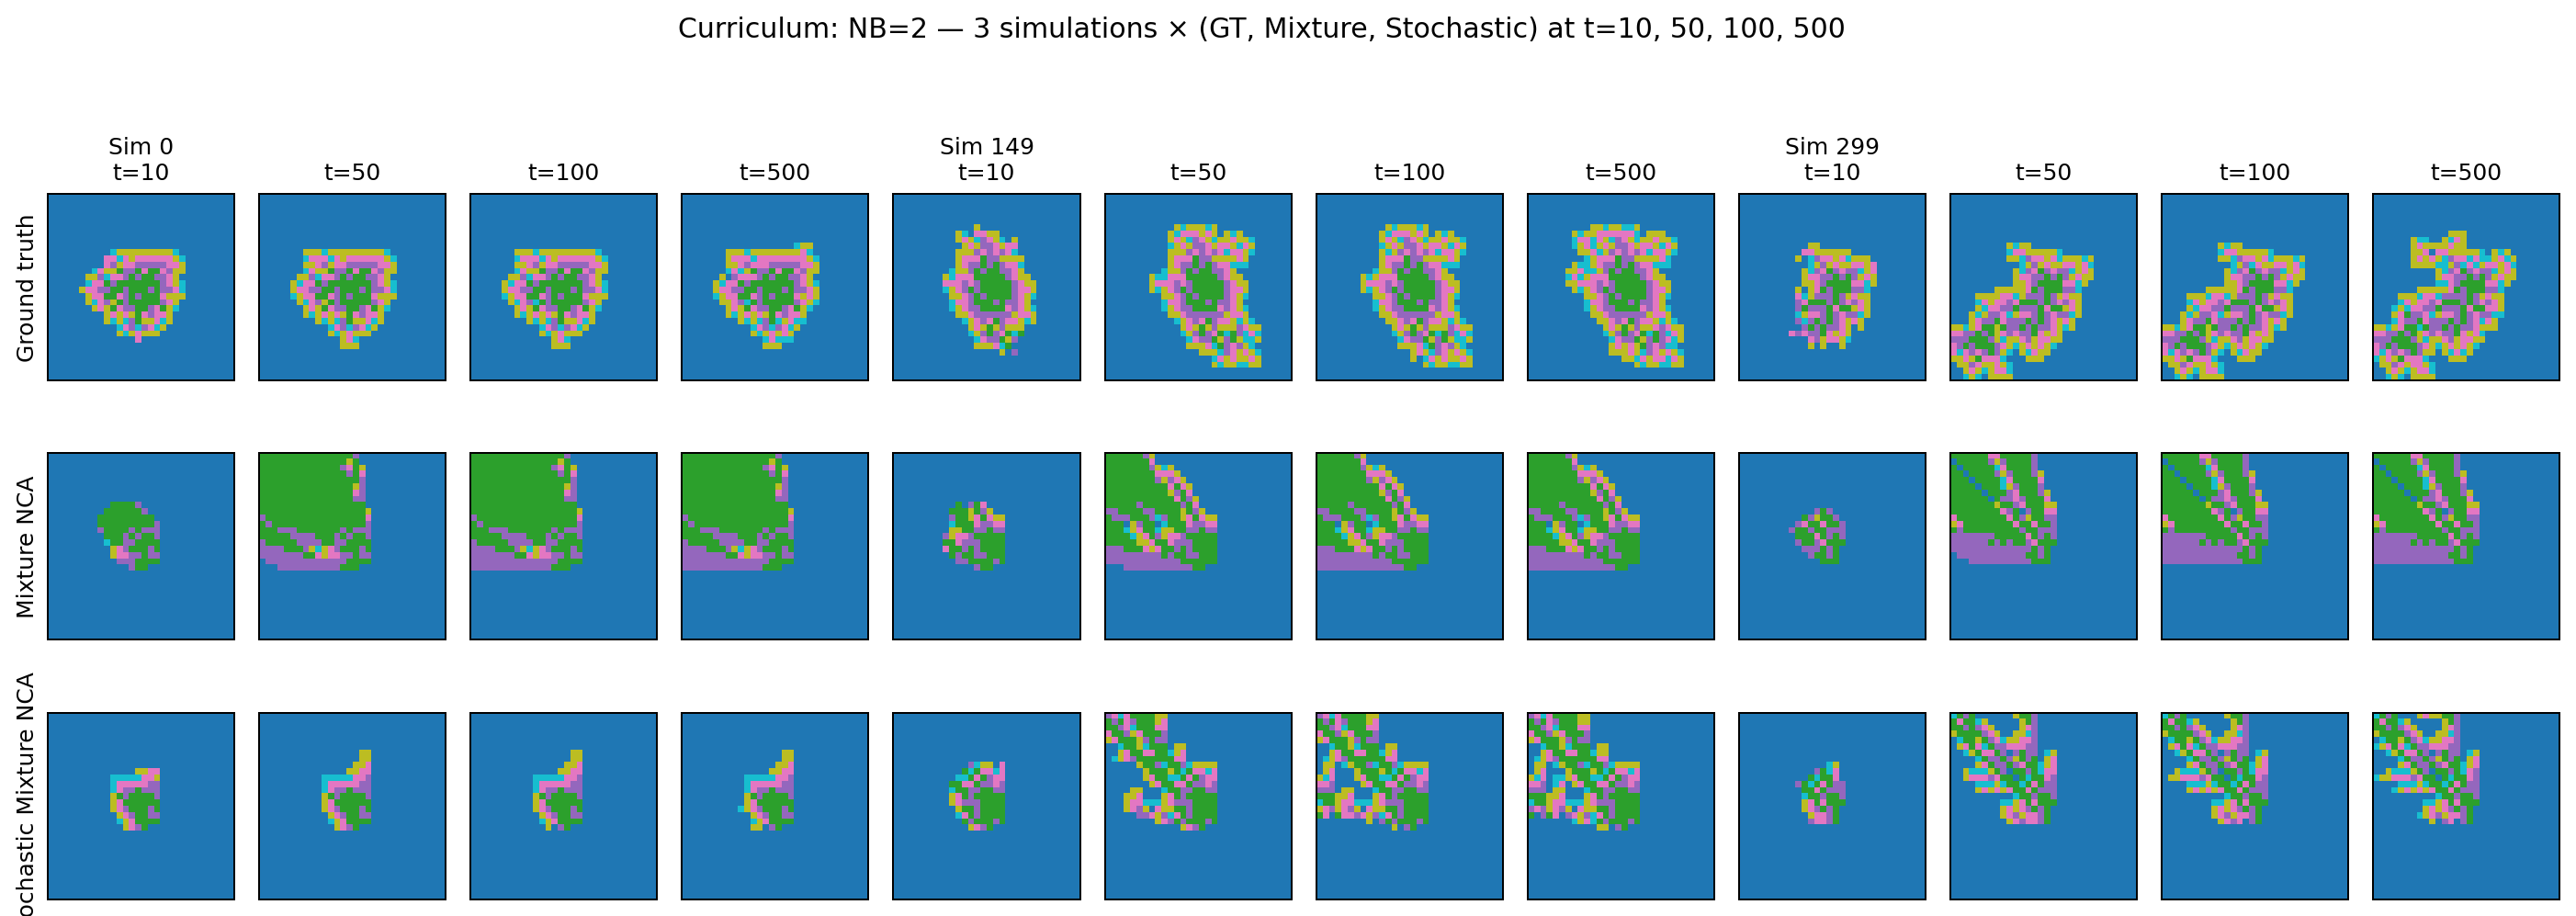
\includegraphics[width=\textwidth]{figs/curriculum/curriculum_examples_NB2.png}
  \caption{Curriculum experiment, \(NB=2\). \textbf{Legend:} three rows = ground truth, Mixture NCA, Stochastic Mixture NCA; four columns = time steps \(t=10,50,100,500\); each block = one of three simulations (same initial state for all three rows).}
  \label{fig:impl:curriculum:ex_nb2}
\end{figure}

\begin{figure}[H]
  \centering
  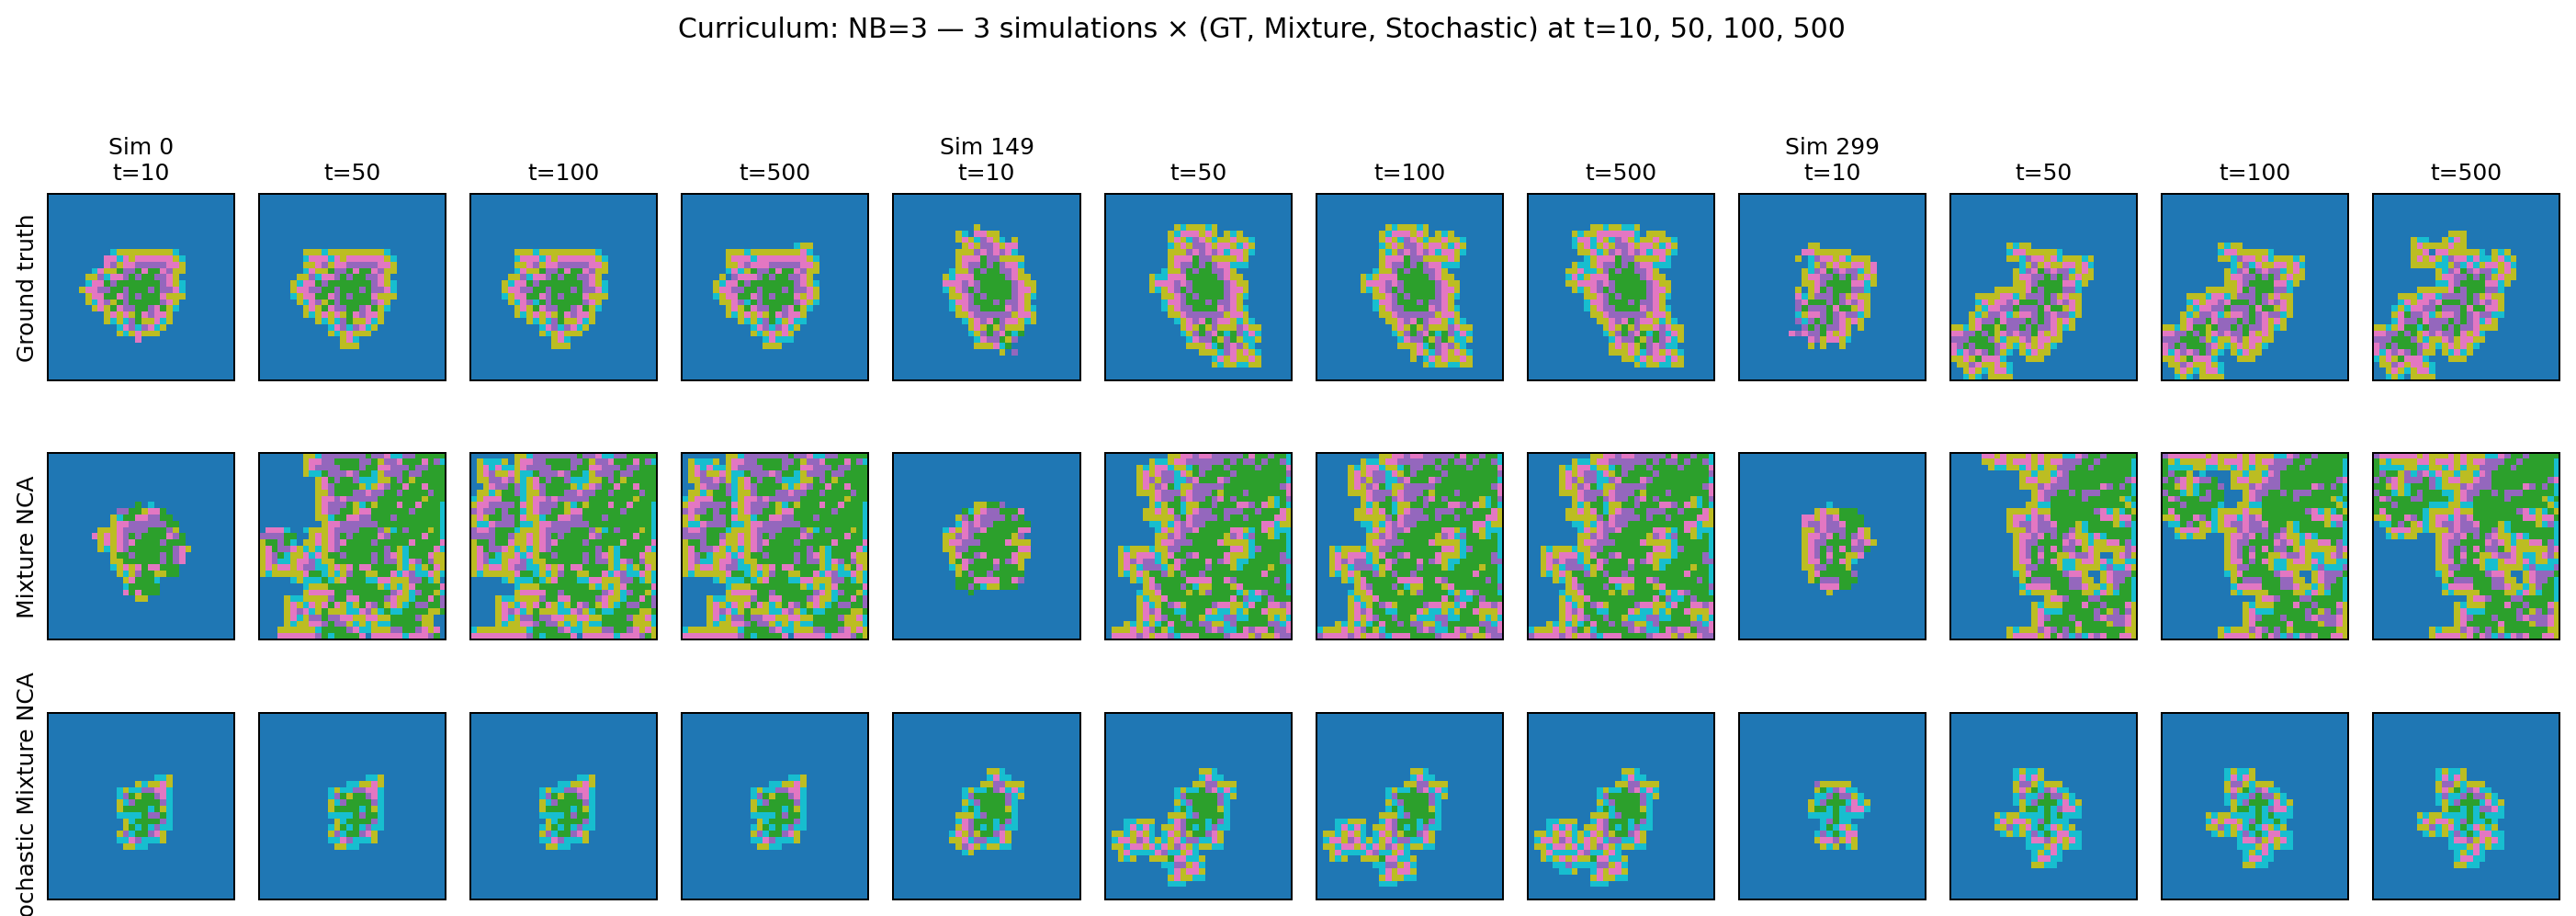
\includegraphics[width=\textwidth]{figs/curriculum/curriculum_examples_NB3.png}
  \caption{Curriculum experiment, \(NB=3\). \textbf{Legend:} same as Figure~\ref{fig:impl:curriculum:ex_nb2} (rows = GT, Mixture NCA, Stochastic; columns = \(t=10,50,100,500\); three simulations).}
  \label{fig:impl:curriculum:ex_nb3}
\end{figure}

\begin{figure}[H]
  \centering
  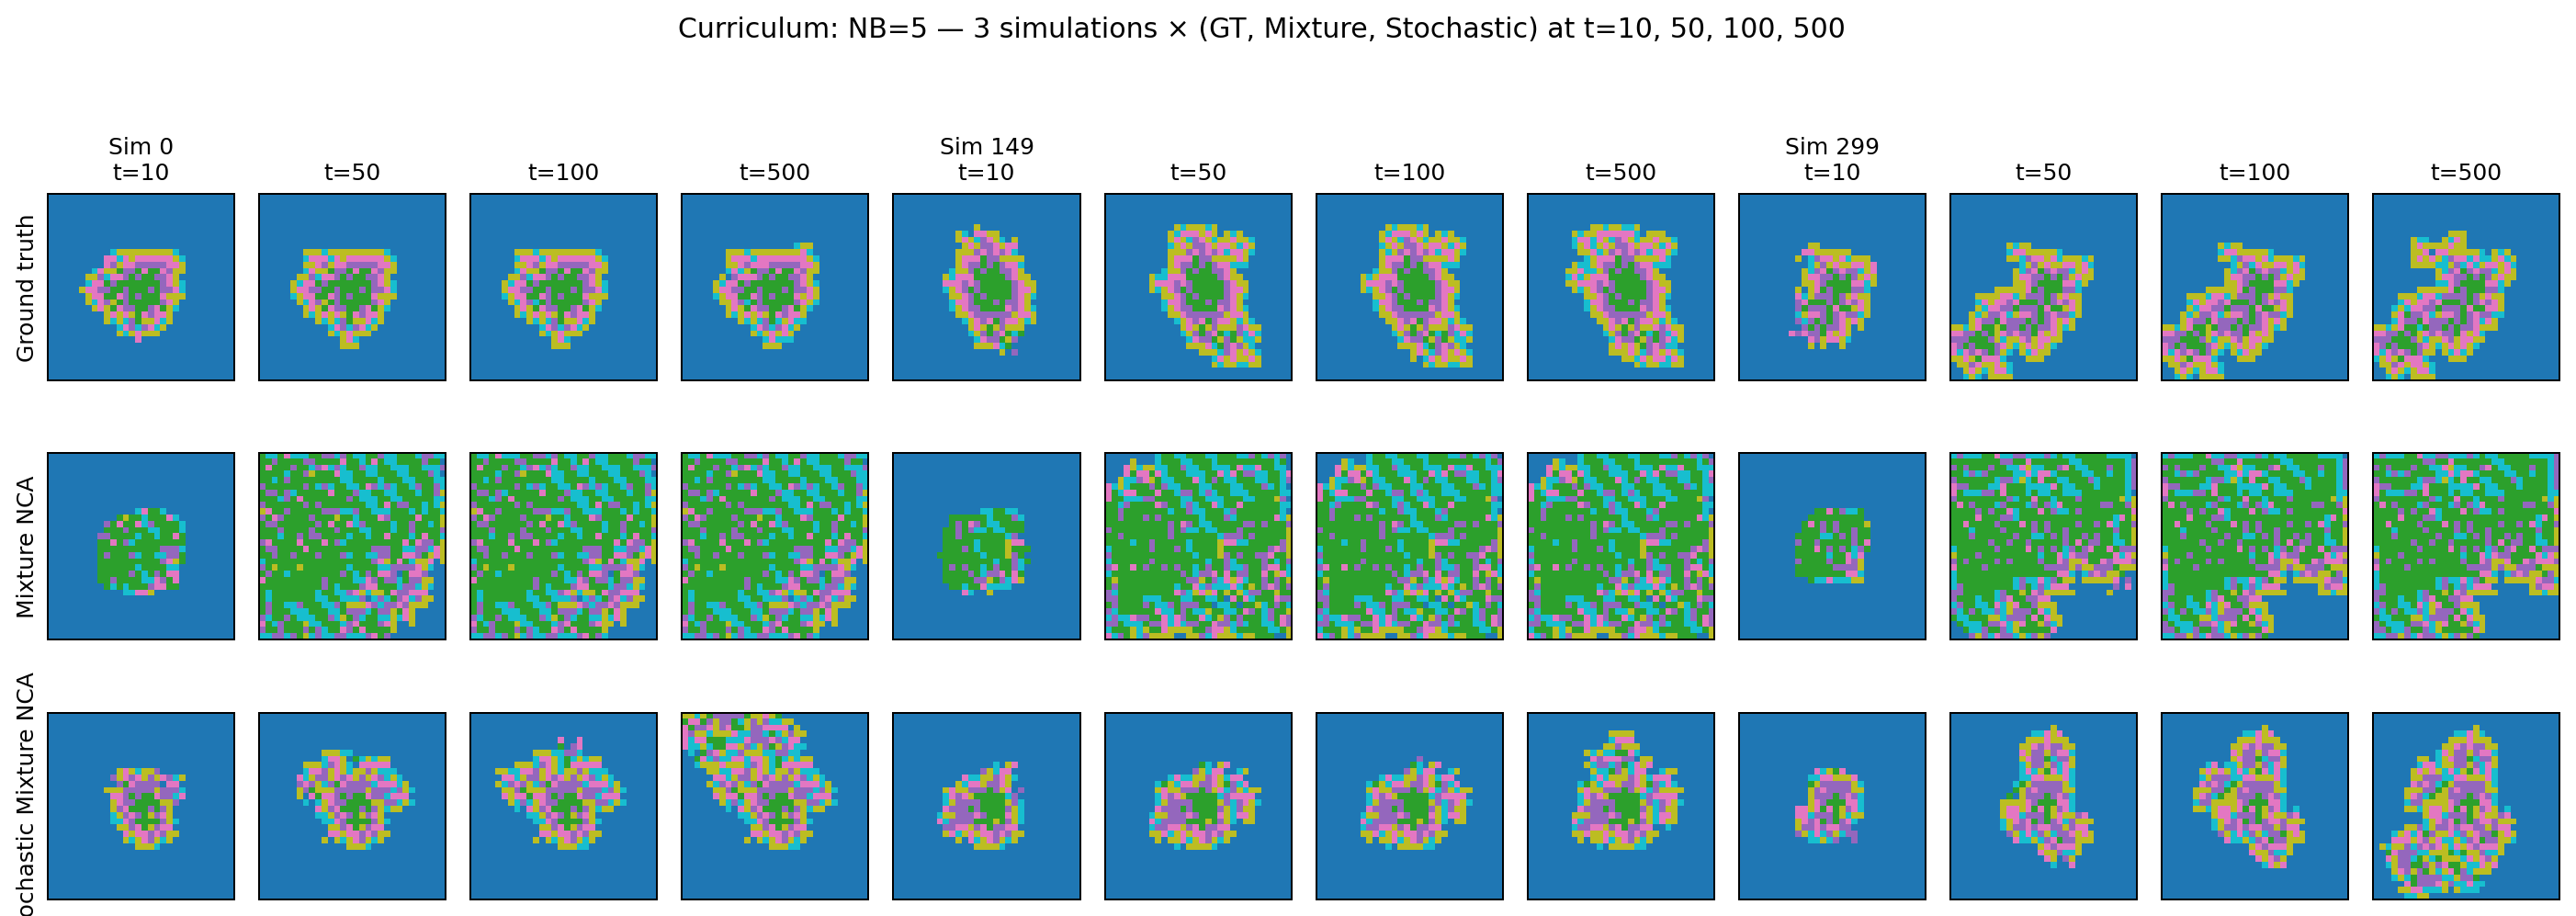
\includegraphics[width=\textwidth]{figs/curriculum/curriculum_examples_NB5.png}
  \caption{Curriculum experiment, \(NB=5\). \textbf{Legend:} same as Figure~\ref{fig:impl:curriculum:ex_nb2} (rows = GT, Mixture NCA, Stochastic; columns = \(t=10,50,100,500\); three simulations).}
  \label{fig:impl:curriculum:ex_nb5}
\end{figure}

\subsubsection{Metric results and interpretation}
\label{sec:results:curriculum:metrics}

After training we run the evaluation protocol (free rollouts at 25, 100, and 500 steps) for each combination of neighbourhood size and step length, and we record the six biological metrics.
Figure~\ref{fig:impl:curriculum:dashboard} reports the \emph{mean} of each metric over the three step lengths (25, 100, 500) for each neighbourhood size and each model; Table~\ref{tab:impl:curriculum:metrics_summary} summarises which configuration is best per metric and explains the contrast between metric types.

\paragraph{Distributional metrics (KL divergence, Chi-square, categorical MMD).}
These metrics measure how closely the \emph{global statistical distribution} of cell states (or derived counts) in the generated pattern matches the ground truth (e.g., proportions of cell types, overall composition).
On all three, \textbf{Stochastic Mixture NCA} clearly outperforms Mixture NCA, and the gap widens as \(NB\) increases: at \(NB=5\) the stochastic model attains the lowest values (e.g., KL and Chi-square roughly halved or better vs.\ the deterministic one; categorical MMD much lower at \(NB=5\)).
The deterministic Mixture NCA improves from \(NB=2\) to \(NB=3\) but then plateaus or slightly degrades (e.g., Chi-square and categorical MMD rise again from \(NB=3\) to \(NB=5\)), as if the larger receptive field does not help it further for distributional fidelity.
The stochastic variant, by contrast, benefits consistently from a larger neighbourhood: it can explore the state space more and, with more context, better approximate the target distribution.

\paragraph{Spatial metrics (tumour size diff, border size diff, spatial variance diff).}
These metrics measure \emph{geometric and structural} accuracy: size of the active region, extent of boundaries, and spatial clustering or dispersion.
Here the picture is more nuanced and the two models behave differently.
\textbf{Mixture NCA} often performs best at \textbf{\(NB=3\)} for border size and spatial variance: the deterministic rule, with a moderate neighbourhood, can form stable local structures and sharp boundaries without the extra variability that stochasticity introduces.
\textbf{Stochastic Mixture NCA} exhibits a pronounced \emph{peak in error at \(NB=3\)} on border size and spatial variance (worse than at \(NB=2\) or \(NB=5\)), suggesting that at this scale the randomness interferes with precise spatial coherence.
At \textbf{\(NB=5\)}, the stochastic model recovers: it improves on tumour size diff, border size diff, and spatial variance diff, and at \(NB=5\) often matches or beats the deterministic model on these spatial metrics, while the deterministic one can degrade (e.g., spatial variance diff rises from \(NB=3\) to \(NB=5\)).
At \(NB=2\), Mixture NCA sometimes has an edge on spatial metrics (e.g., tumour size diff), but both models are less stable at long horizons when \(NB\) is small.

\paragraph{Why distributional and spatial metrics give different results.}
Distributional metrics aggregate over the whole pattern and reward a good match of \emph{overall} counts and proportions; they benefit from the stochastic model's ability to explore and from a larger receptive field (\(NB=5\)), which provides more context for consistent long-horizon behaviour.
Spatial metrics, in contrast, are sensitive to \emph{local} geometry: sharp borders, coherent regions, and stable spatial arrangement.
Stochasticity can help globally but add local ``noise'' or blurring, which hurts border and spatial-variance accuracy at an intermediate scale (\(NB=3\)); the deterministic model, with no sampling noise, can excel at that scale for structure.
When \(NB\) is increased to 5, the stochastic model gains enough context to stabilise its spatial behaviour (or the randomness averages out better), so it recovers and often surpasses the deterministic one even on spatial metrics.
Hence there is no single ``best'' \(NB\) or model for all metrics: the choice depends on whether one prioritises distributional agreement (favor Stochastic Mixture NCA and \(NB=5\)) or fine-grained spatial fidelity at a given scale (where \(NB=3\) can be best for the deterministic model, and \(NB=5\) for the stochastic one).

\paragraph{How the metrics change with step length.}
We evaluate at 25, 100, and 500 steps to see how performance changes as the rollout gets longer.
At \textbf{25 steps} we are close to what the model saw in the first curriculum phase (35-step windows), so errors stay low and the difference between \(NB=2\), \(NB=3\), and \(NB=5\) is small.
At \textbf{100} and \textbf{500 steps} the metrics generally worsen and the receptive field matters more: distributional metrics are clearly best for \(NB=5\), especially for the stochastic model; spatial metrics show the trade-offs described above (e.g., Mixture NCA best at \(NB=3\) for some, Stochastic best at \(NB=5\) after recovering from the \(NB=3\) peak).
Figure~\ref{fig:impl:curriculum:categorical_mmd} breaks out categorical MMD by step length; the dashboard (Figure~\ref{fig:impl:curriculum:dashboard}) averages over step lengths and gives the overall picture.

\paragraph{Comparison with Step 3.}
In Step 3 we had 300 trajectories of 100 steps, no curriculum, and we evaluated at 25, 50, and 100 steps with \(NB\) from 1 to 7.
Here we have 300 trajectories of 500 steps, a three-phase curriculum (35, 100, 500), and we evaluate at 25, 100, and 500 steps with \(NB \in \{2,3,5\}\).
The conclusions match: in both experiments, larger neighbourhoods help on distributional metrics at longer horizons, and no single \(NB\) is best on every metric.
Step 3 showed that \(NB=1\) is too small and that \(NB\ge2\) gives a clear improvement; this curriculum run shows that among 2, 3, and 5, the larger one (\(NB=5\)) is better at 100 and 500 steps, especially for the stochastic model.
We use the same six metrics in both experiments, so the comparison is fair; the curriculum experiment simply pushes the evaluation horizon to 500 steps and confirms that the neighbourhood-size effect is still there.

\begin{figure}[H]
  \centering
  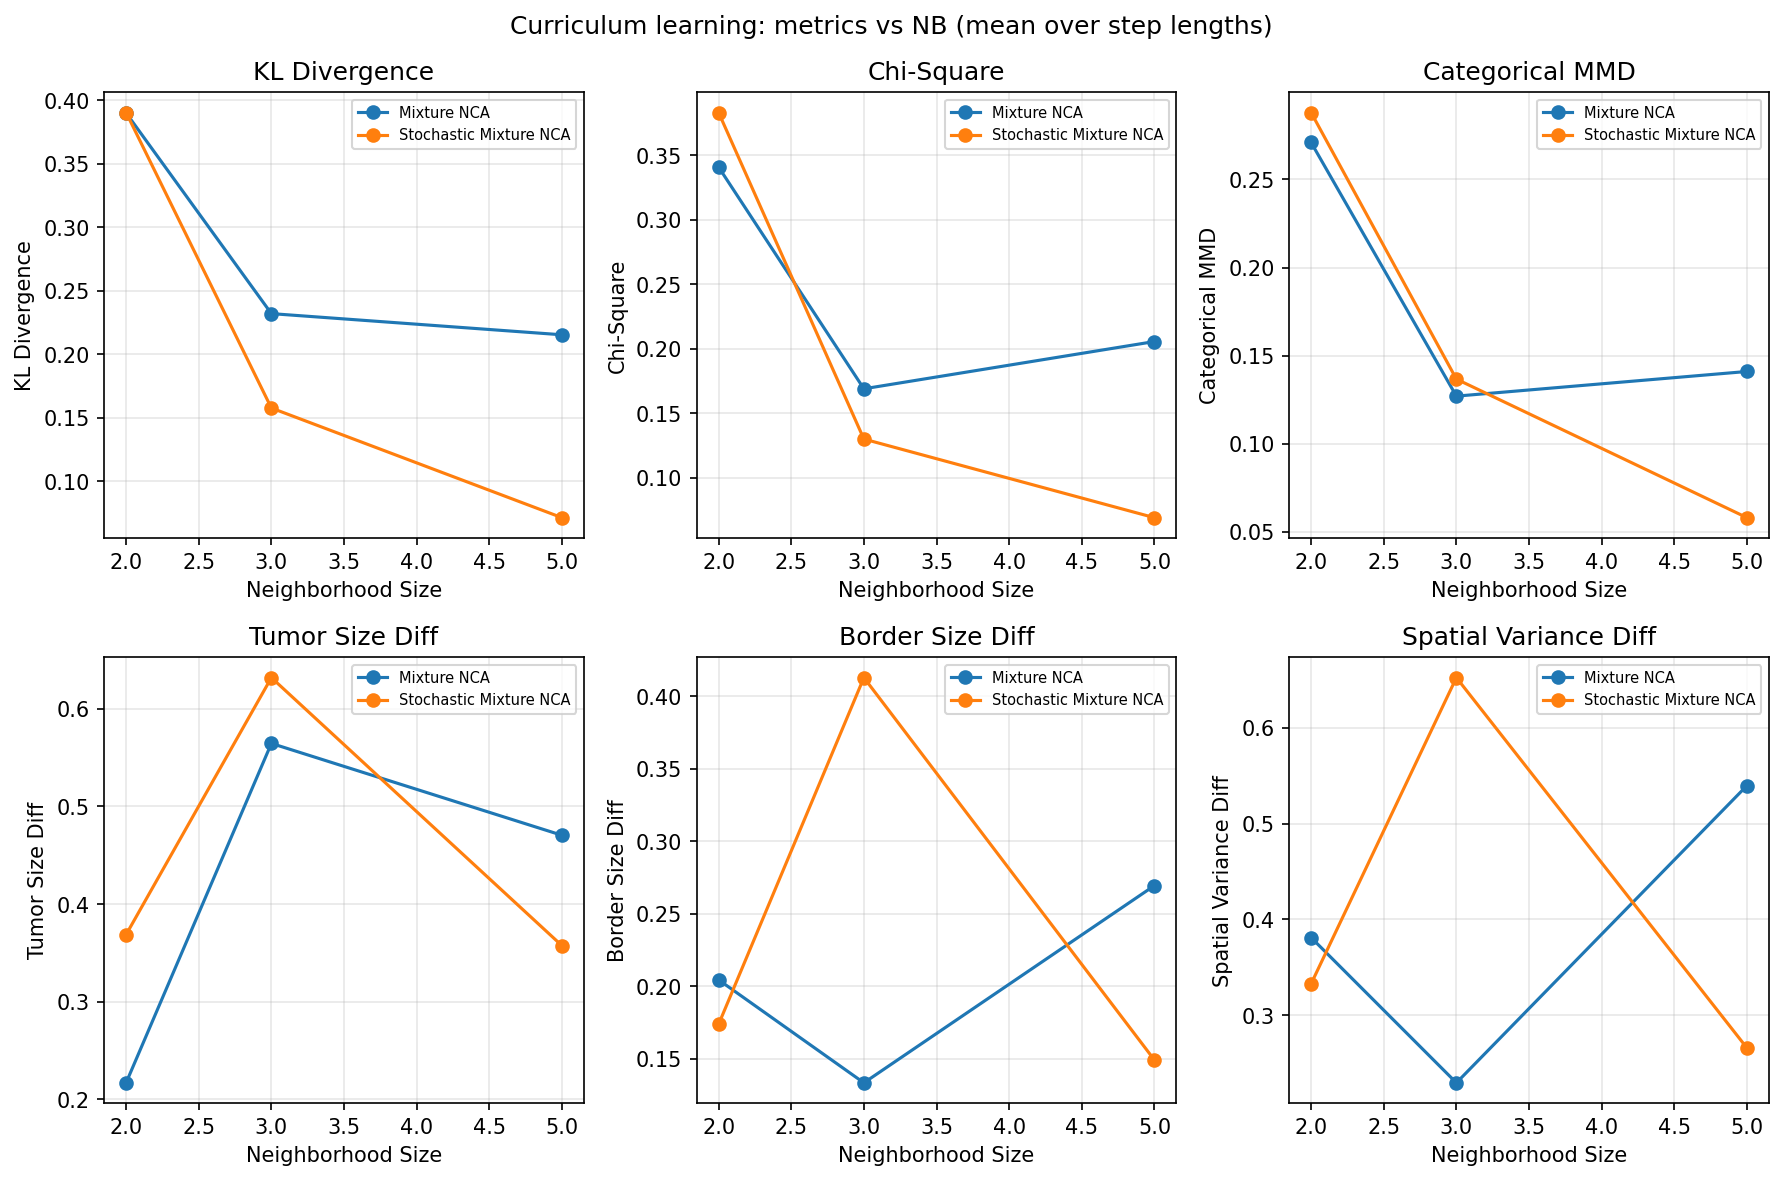
\includegraphics[width=\textwidth]{figs/curriculum/curriculum_dashboard.png}
  \caption{Curriculum experiment: mean metric values vs.\ neighbourhood size. \textbf{Legend:} six panels = KL divergence, Chi-square, categorical MMD (top), tumour size diff, border size diff, spatial variance diff (bottom); abscissa = \(NB\); ordinate = mean over step lengths 25, 100, 500 (lower is better); series = Mixture vs.\ Stochastic Mixture NCA.}
  \label{fig:impl:curriculum:dashboard}
\end{figure}

% Summary of curriculum experiment: best configuration per metric (mean over step lengths 25, 100, 500)
\begin{table}[H]
\centering
\small
\begin{tabulary}{\textwidth}{lLLL}
\toprule
Metric & Type & Mixture NCA (best \(NB\)) & Stochastic Mixture NCA (best \(NB\)) \\
\midrule
KL Divergence & Distributional & \(NB=5\) (plateau after \(NB=3\)) & \(NB=5\) (lowest; large gain vs.\ det.) \\
Chi-Square & Distributional & \(NB=3\) (degrades at \(NB=5\)) & \(NB=5\) (lowest) \\
Categorical MMD & Distributional & \(NB=3\) (slight rise at \(NB=5\)) & \(NB=5\) (lowest) \\
\midrule
Tumor Size Diff & Spatial & \(NB=2\) (peaks at \(NB=3\)) & \(NB=5\) (recovers after \(NB=3\) peak) \\
Border Size Diff & Spatial & \(NB=3\) (best) & \(NB=5\) (poor at \(NB=3\), then recovers) \\
Spatial Variance Diff & Spatial & \(NB=3\) (best; worsens at \(NB=5\)) & \(NB=5\) (peak at \(NB=3\), then best) \\
\bottomrule
\end{tabulary}
\caption{Curriculum experiment: summary of which neighborhood size yields the best mean value (over step lengths 25, 100, 500) for each metric and model. ``Type'' distinguishes distributional (global statistics) vs.\ spatial (geometry/structure). The deterministic model often peaks at \(NB=3\) on spatial metrics; the stochastic model peaks in error at \(NB=3\) on spatial metrics then improves at \(NB=5\).}
\label{tab:impl:curriculum:metrics_summary}
\end{table}


\paragraph{Why we see these values.}
The model is trained on windows of 35, 100, and 500 steps, so it learns to match the data over longer and longer horizons.
But at evaluation we use free rollouts: the model has to stay coherent for 25, 100, or 500 steps without ever seeing the true state again after the start.
Short rollouts (25 steps) are close to the first training phase, so all three neighbourhood sizes do well and the gap between them is small.

When we go to 100 and 500 steps, errors build up and the receptive field matters more: a larger neighbourhood (\(NB=5\)) gives the update rule more context, which helps keep the tissue consistent (hence better KL and Chi-square) and, for the stochastic model, keeps rule choices more stable over time (hence the clearer win for \(NB=5\) at long horizons).
The deterministic Mixture NCA mixes rules in a soft way, so it is less sensitive to sampling noise but can still drift over long rollouts; depending on the metric and the horizon, we sometimes see \(NB=3\) best for border or spatial variance and \(NB=5\) best for KL and categorical MMD.

Figure~\ref{fig:impl:curriculum:categorical_mmd} zooms in on categorical MMD as we change neighbourhood size and step length.
At \textbf{25 steps} both models achieve low MMD for all \(NB\); the curve is often U-shaped with a minimum at \(NB=3\) for Mixture NCA, and similar for the stochastic variant.
At \textbf{100} and \textbf{500 steps} the two models diverge: \textbf{Stochastic Mixture NCA} shows a monotonic decrease in MMD as \(NB\) increases, reaching the lowest values at \(NB=5\) (around 0.04 to 0.05), whereas \textbf{Mixture NCA} again exhibits a U-shaped trend with minimum at \(NB=3\) and a rise at \(NB=5\) (especially at 500 steps).
So for this distributional metric at long horizons, the stochastic model benefits consistently from a larger receptive field, while the deterministic one does not improve beyond \(NB=3\) and can even degrade. This is consistent with the dashboard and with the interpretation that stochasticity plus context (\(NB=5\)) yields better global distributional match.

\begin{figure}[H]
  \centering
  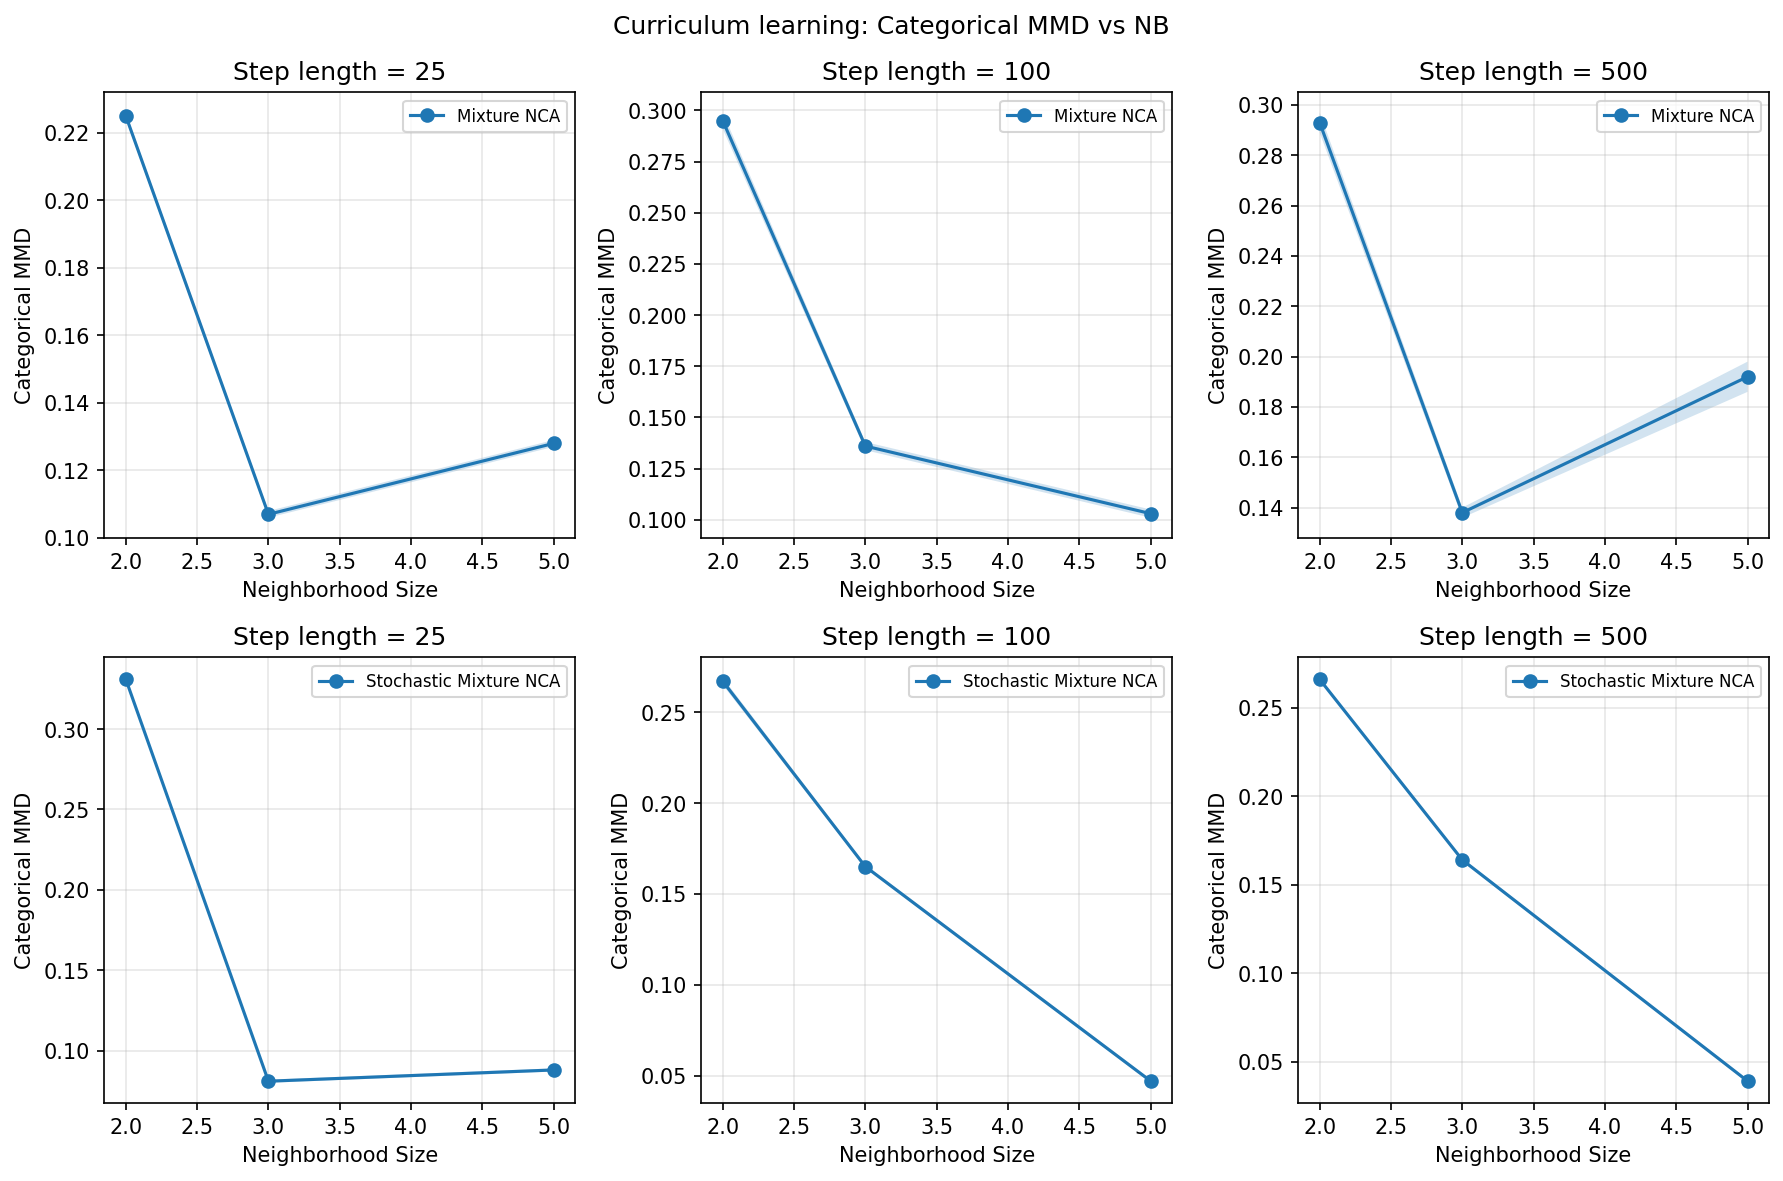
\includegraphics[width=\textwidth]{figs/curriculum/curriculum_metric_vs_nb_categorical_mmd.png}
  \caption{Curriculum experiment: categorical MMD vs.\ neighbourhood size. \textbf{Legend:} columns = step length (25, 100, 500); top row = Mixture NCA, bottom row = Stochastic Mixture NCA; abscissa = \(NB\), ordinate = categorical MMD (lower is better).}
  \label{fig:impl:curriculum:categorical_mmd}
\end{figure}

The training loss curves (Figure~\ref{fig:impl:curriculum:loss}) show that both models converge quickly: on a linear scale the loss drops to values near zero within the first phase and the three neighbourhood sizes are almost indistinguishable.
Figure~\ref{fig:impl:curriculum:loss_log} plots the same data on a log scale so that the initial drop (by several orders of magnitude) and small differences are visible.
On the log scale we see sharp \emph{spikes} at curriculum phase transitions (e.g., when the window length or learning rate changes): the loss jumps up briefly then returns to a low plateau.
The Stochastic Mixture NCA tends to show more frequent and sometimes higher spikes than the deterministic model in the early phases, likely because sampling introduces extra variability when the task changes.
Around step 100 (concatenated) there is a clear jump to a slightly higher plateau for all \(NB\); \(NB=2\) settles at a marginally higher loss than \(NB=3\) and \(NB=5\) for both models.
Importantly, training loss is computed with teacher forcing, so it does not reflect long-horizon free-rollout behaviour; the real differences across \(NB\) and between models show up at evaluation (Figures~\ref{fig:impl:curriculum:dashboard} and \ref{fig:impl:curriculum:categorical_mmd}).
We do not compute a validation loss in this run; early stopping uses only the training loss (patience 20 epochs per phase).

\begin{figure}[H]
  \centering
  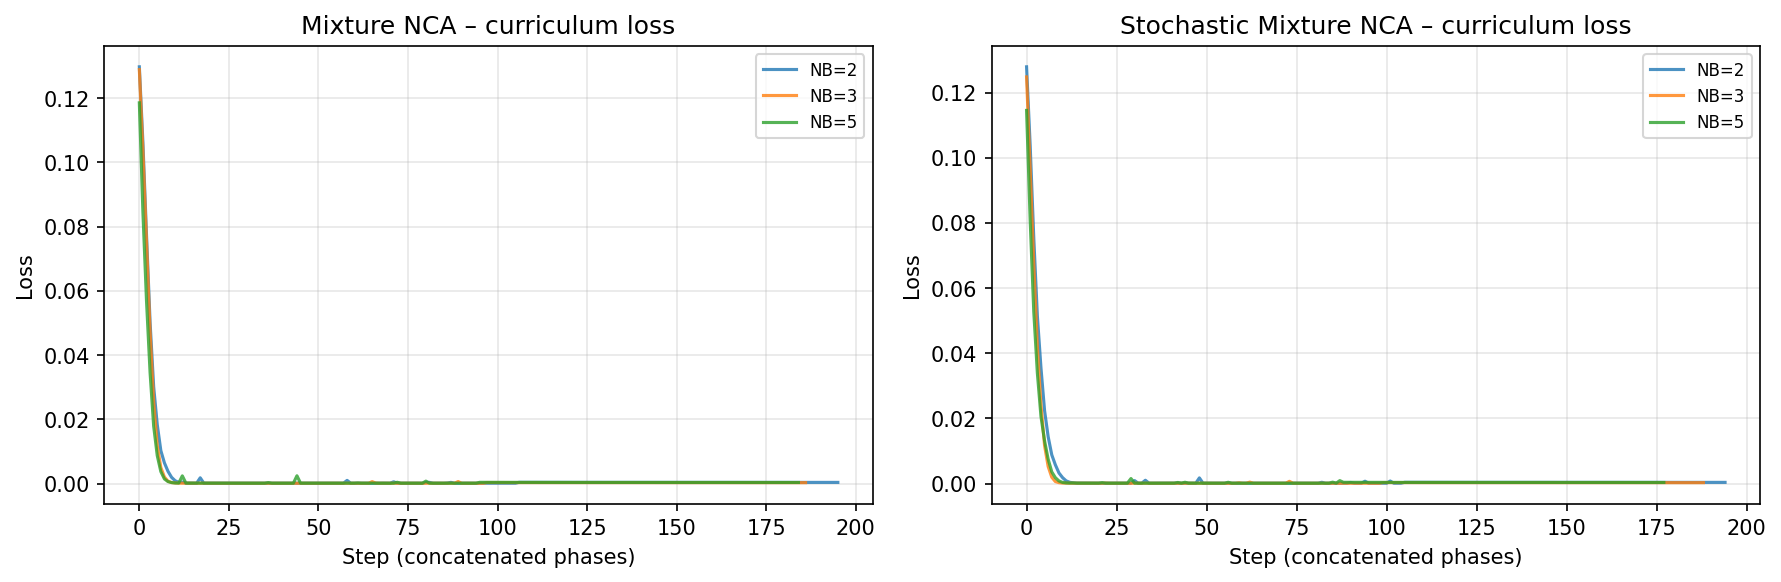
\includegraphics[width=\textwidth]{figs/curriculum/curriculum_loss_curves.png}
  \caption{Curriculum experiment: training loss (linear scale) over curriculum phases. \textbf{Legend:} left panel = Mixture NCA, right = Stochastic Mixture NCA; abscissa = training step; ordinate = loss; one curve per \(NB\in\{2,3,5\}\).}
  \label{fig:impl:curriculum:loss}
\end{figure}

\begin{figure}[H]
  \centering
  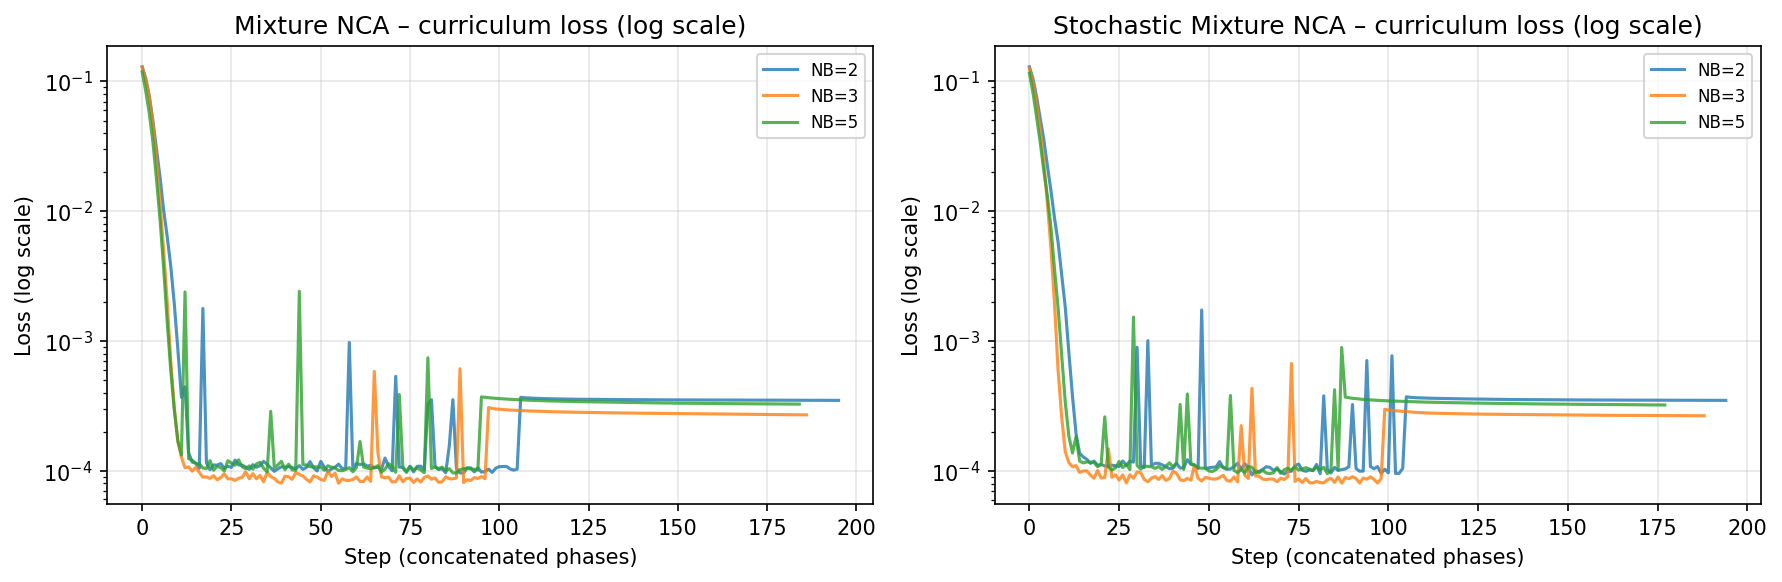
\includegraphics[width=\textwidth]{figs/curriculum/curriculum_loss_curves_log.png}
  \caption{Curriculum experiment: same as Figure~\ref{fig:impl:curriculum:loss} with log-scale ordinate. \textbf{Legend:} same layout (left = Mixture, right = Stochastic; curves = \(NB=2,3,5\)).}
  \label{fig:impl:curriculum:loss_log}
\end{figure}

\subsubsection{Why generated images differ from ground truth}
\label{sec:results:curriculum:limitations}

When we look at the qualitative figures (Figures~\ref{fig:impl:curriculum:ex_nb2} to \ref{fig:impl:curriculum:ex_nb5}), we see that the stochastic variant stays close to the ground truth for \(NB=3\) and \(NB=5\) at all time points, with controlled growth and organic shapes; at \(NB=2\) it still keeps the right scale but the internal structure can look noisier.
The deterministic Mixture NCA, on the other hand, matches the ground truth only early on (around \(t=10\)). As time goes on it starts to diverge: the pattern expands in an uncontrolled way, becomes blocky and homogeneous, and by \(t=500\) the generated tissue often has a different layout, a different mix of cell types, and a tendency to fill the grid instead of evolving like the simulator.

Several factors contribute.
During training we use teacher forcing: at every step we feed the model the true state from the dataset, so small errors do not accumulate and the loss can stay low.
At evaluation we do the opposite: we run free rollouts, where the model only sees its own previous output. In that regime, a small mistake at step 10 is fed into step 11, and the error can grow over time. By step 500 the trajectory may have drifted far from the ground truth even if the model had learned the short-term dynamics well.
A second point is what we actually optimise: the loss is a step-by-step mean squared error over the training window, which encourages correct one-step predictions but does not directly reward how well a long unrolled trajectory matches a single ground-truth run.
For the stochastic model there is an extra nuance: at each step we sample a rule, so different random seeds produce different trajectories; the ground truth we compare against is just one possible realisation of the simulator, and part of the ``difference'' we see is therefore normal variability between runs, not only a failure of the model.
Finally, the last curriculum phase uses 500-step windows but with fewer epochs and a smaller learning rate, so we may stop before the model has fully learned to stay on track for the full 500 steps.

Several directions could be explored to reduce the gap at long times (see also \cref{sec:conc:future}): training longer on 500-step windows or adding more curriculum phases; computing a validation loss with free rollouts and using it for early stopping; adding losses that target the final state of a rollout; or using scheduled teacher forcing so that during training the model gradually sees the true state less often.
At evaluation, running multiple rollouts and averaging or selecting among them could improve the metrics.
The current experiment already shows that the neighbourhood-size effect carries over to the long-horizon curriculum setting and that a larger \(NB\) helps at 100 and 500 steps, especially for the stochastic model.

%-------------------------------------------------------------------
\section{Why evaluation protocol matters}
\label{sec:results:evaluation}
%-------------------------------------------------------------------

A methodological result of this thesis is that \textbf{the evaluation protocol matters}: it can determine whether neighbourhood effects are visible at all. Neighbourhood comparisons are most interpretable when:
\begin{enumerate}
\item training and evaluation are aligned in terms of rule-selection behaviour (e.g., consistent sampling/temperature decisions), and
\item models are evaluated at \textbf{multiple rollout horizons}, because some neighbourhood differences only emerge as errors accumulate over time.
\end{enumerate}

This point is central to the thesis takeaway: if the model already fails because of train--test mismatch (e.g.\ heavy reliance on teacher forcing during training but free rollout at evaluation), neighbourhood effects can be \textbf{masked} by broader instability.

%-------------------------------------------------------------------
\section{Segmentation on BBBC031 (synthetic benchmark)}
\label{sec:results:bbbc031}
%-------------------------------------------------------------------

To complement the synthetic tissue experiments, the thesis also evaluates the extended Stochastic Mixture NCA on the synthetic cell-imaging benchmark BBBC031 (\cref{sec:impl:bbbc031}), where the model must ``grow'' a segmentation mask from seed points (cell centroids) toward a fixed ground-truth target.
In that experiment each model is trained on one image and evaluated on the same image (in-sample); generalization to held-out images is not assessed.

\subsection{Loss curves and optimisation stability}

Training with the default learning rate (\(10^{-3}\)) and 4000 steps yields a clear asymmetry: \(NB=3\) converges to low loss on all five images, while \(NB=7\) either diverges (two images) or settles at much higher loss (three images).
We therefore consider additional training schedules for \(NB=7\) (described in \cref{sec:impl:bbbc031:schedules}); unless stated otherwise, the \(NB=7\) results reported below refer to the re-trained run (lower learning rate, 6000 steps).

\begin{figure}[H]
  \centering
  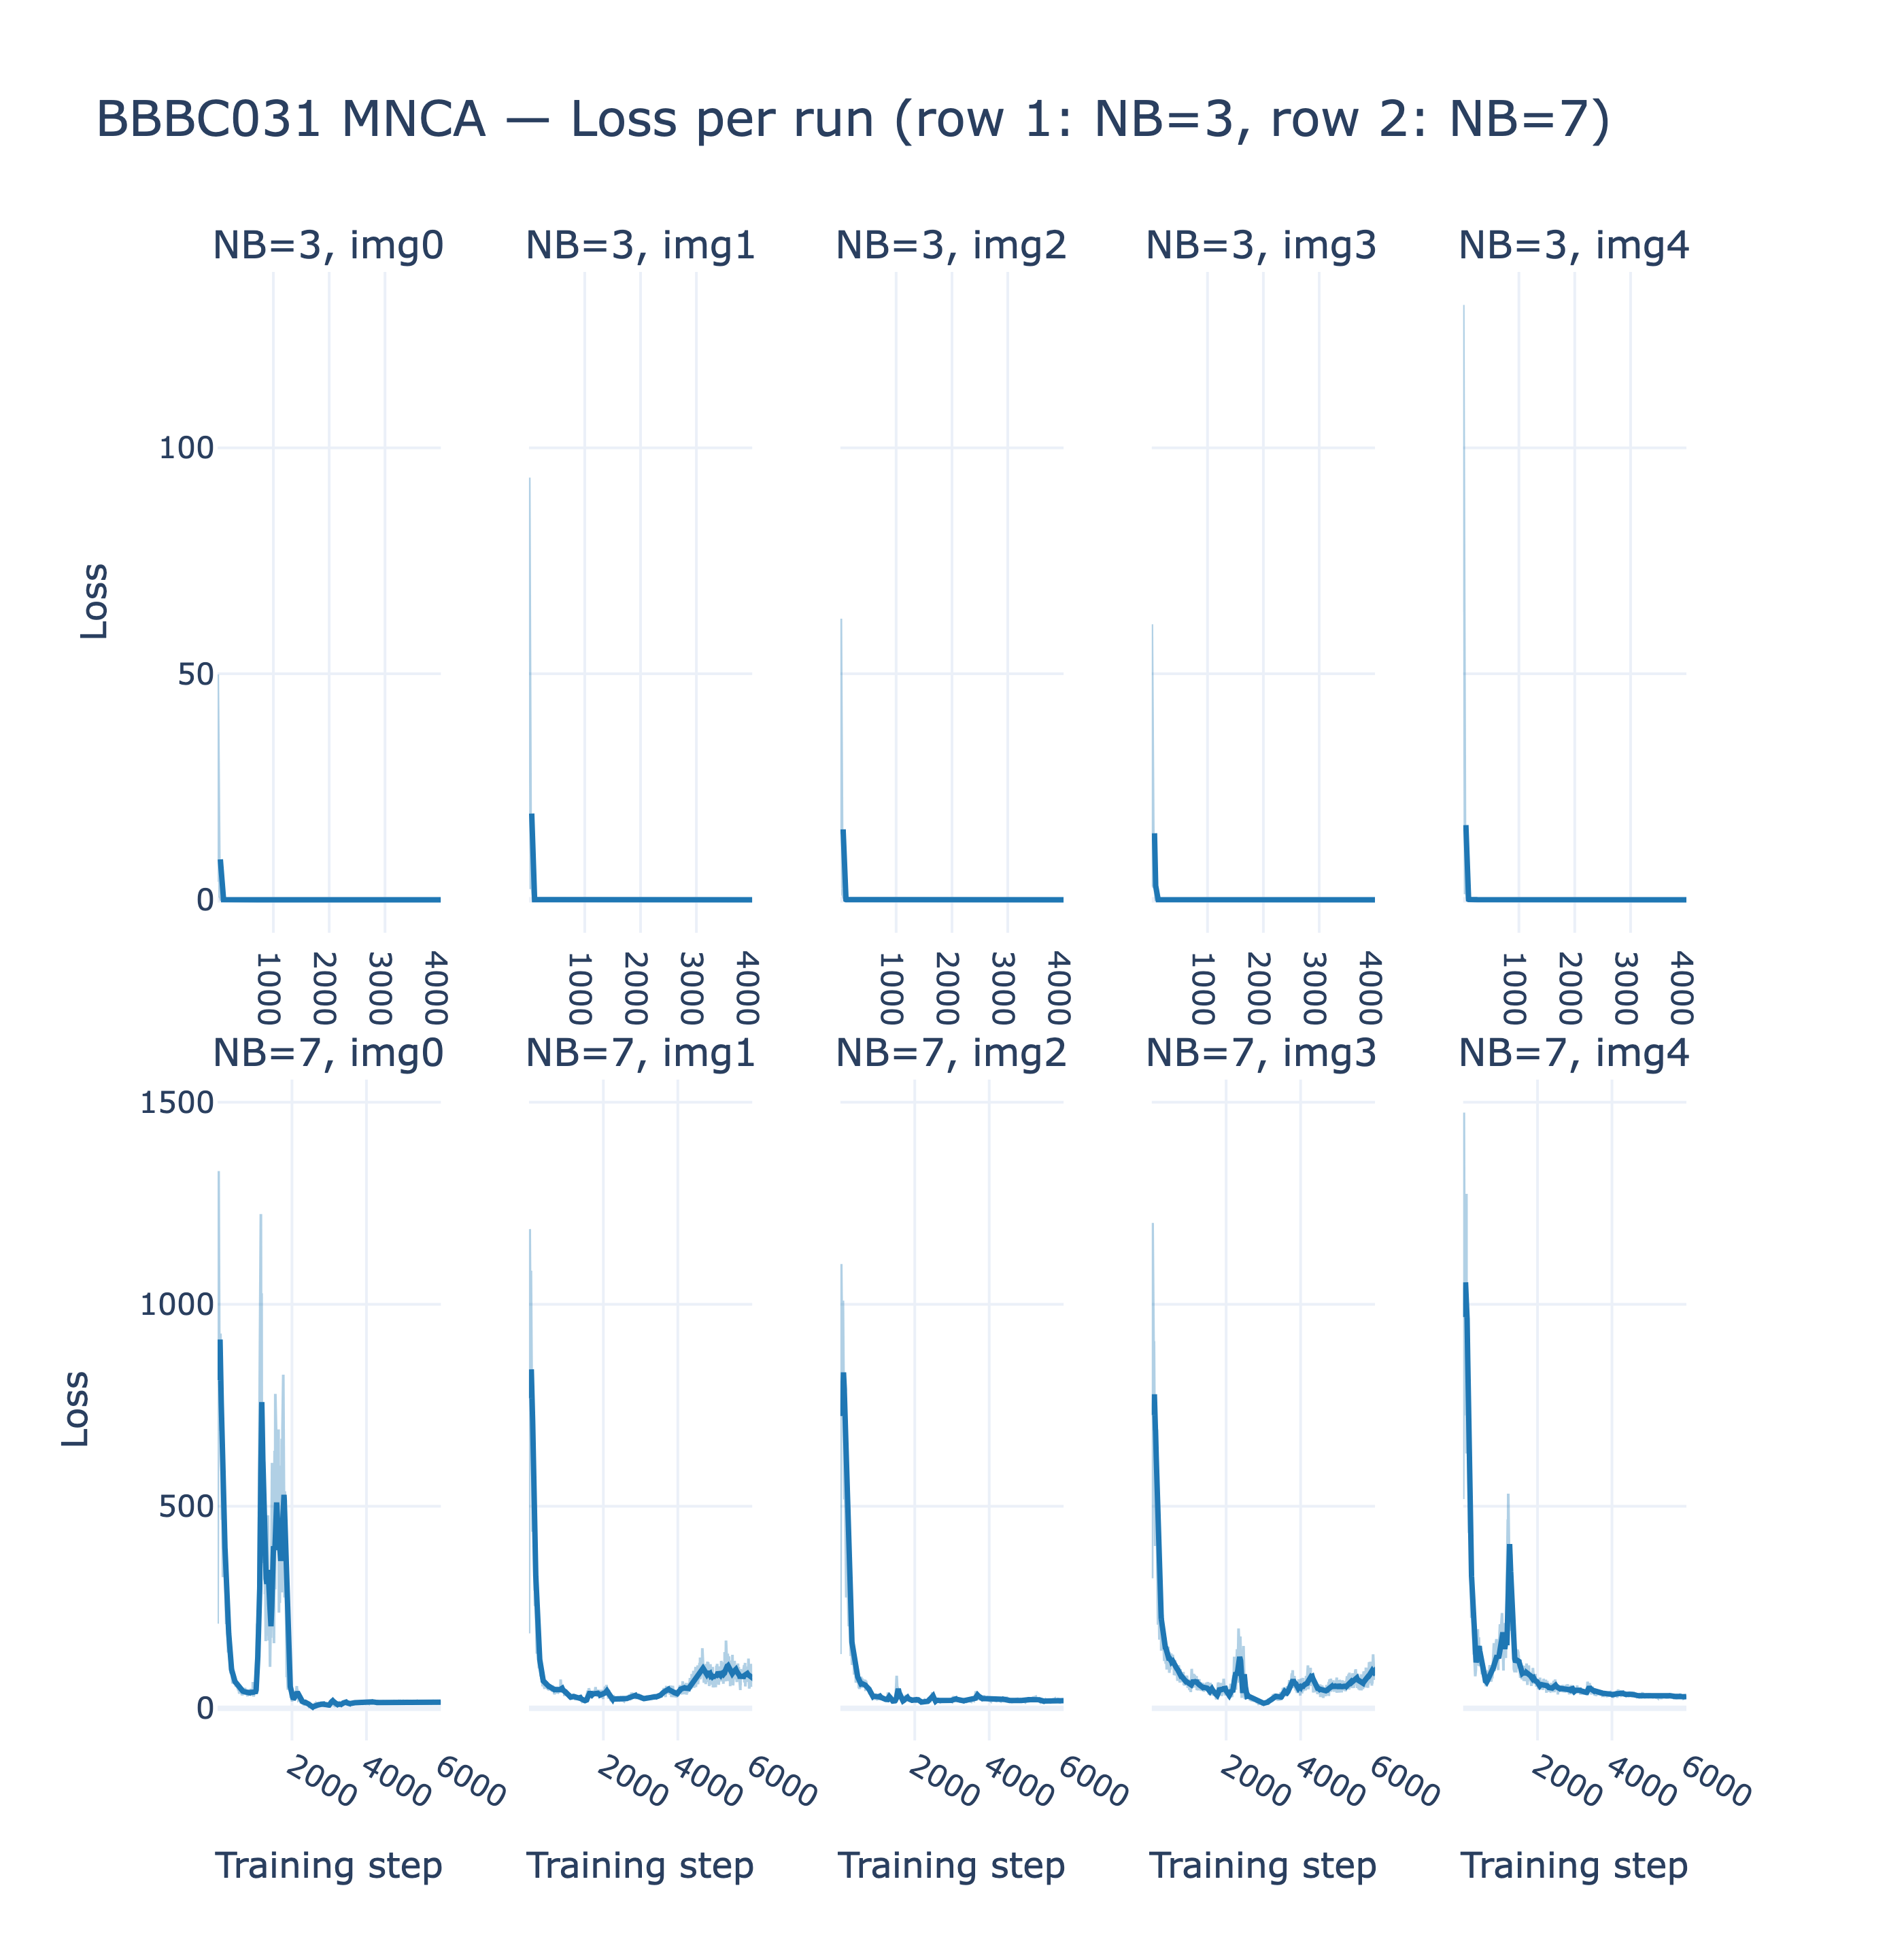
\includegraphics[width=\textwidth]{figs/bbbc031/bbbc031_loss_curves.png}
  \caption{BBBC031: training loss per run. \textbf{Legend:} top row = \(NB=3\) (five images img0--img4, 4000 steps); bottom row = \(NB=7\) re-trained (five images, 6000 steps); abscissa = training step; ordinate = loss; one subplot per image.}
  \label{fig:impl:bbbc031:loss_curves}
\end{figure}

\begin{figure}[H]
  \centering
  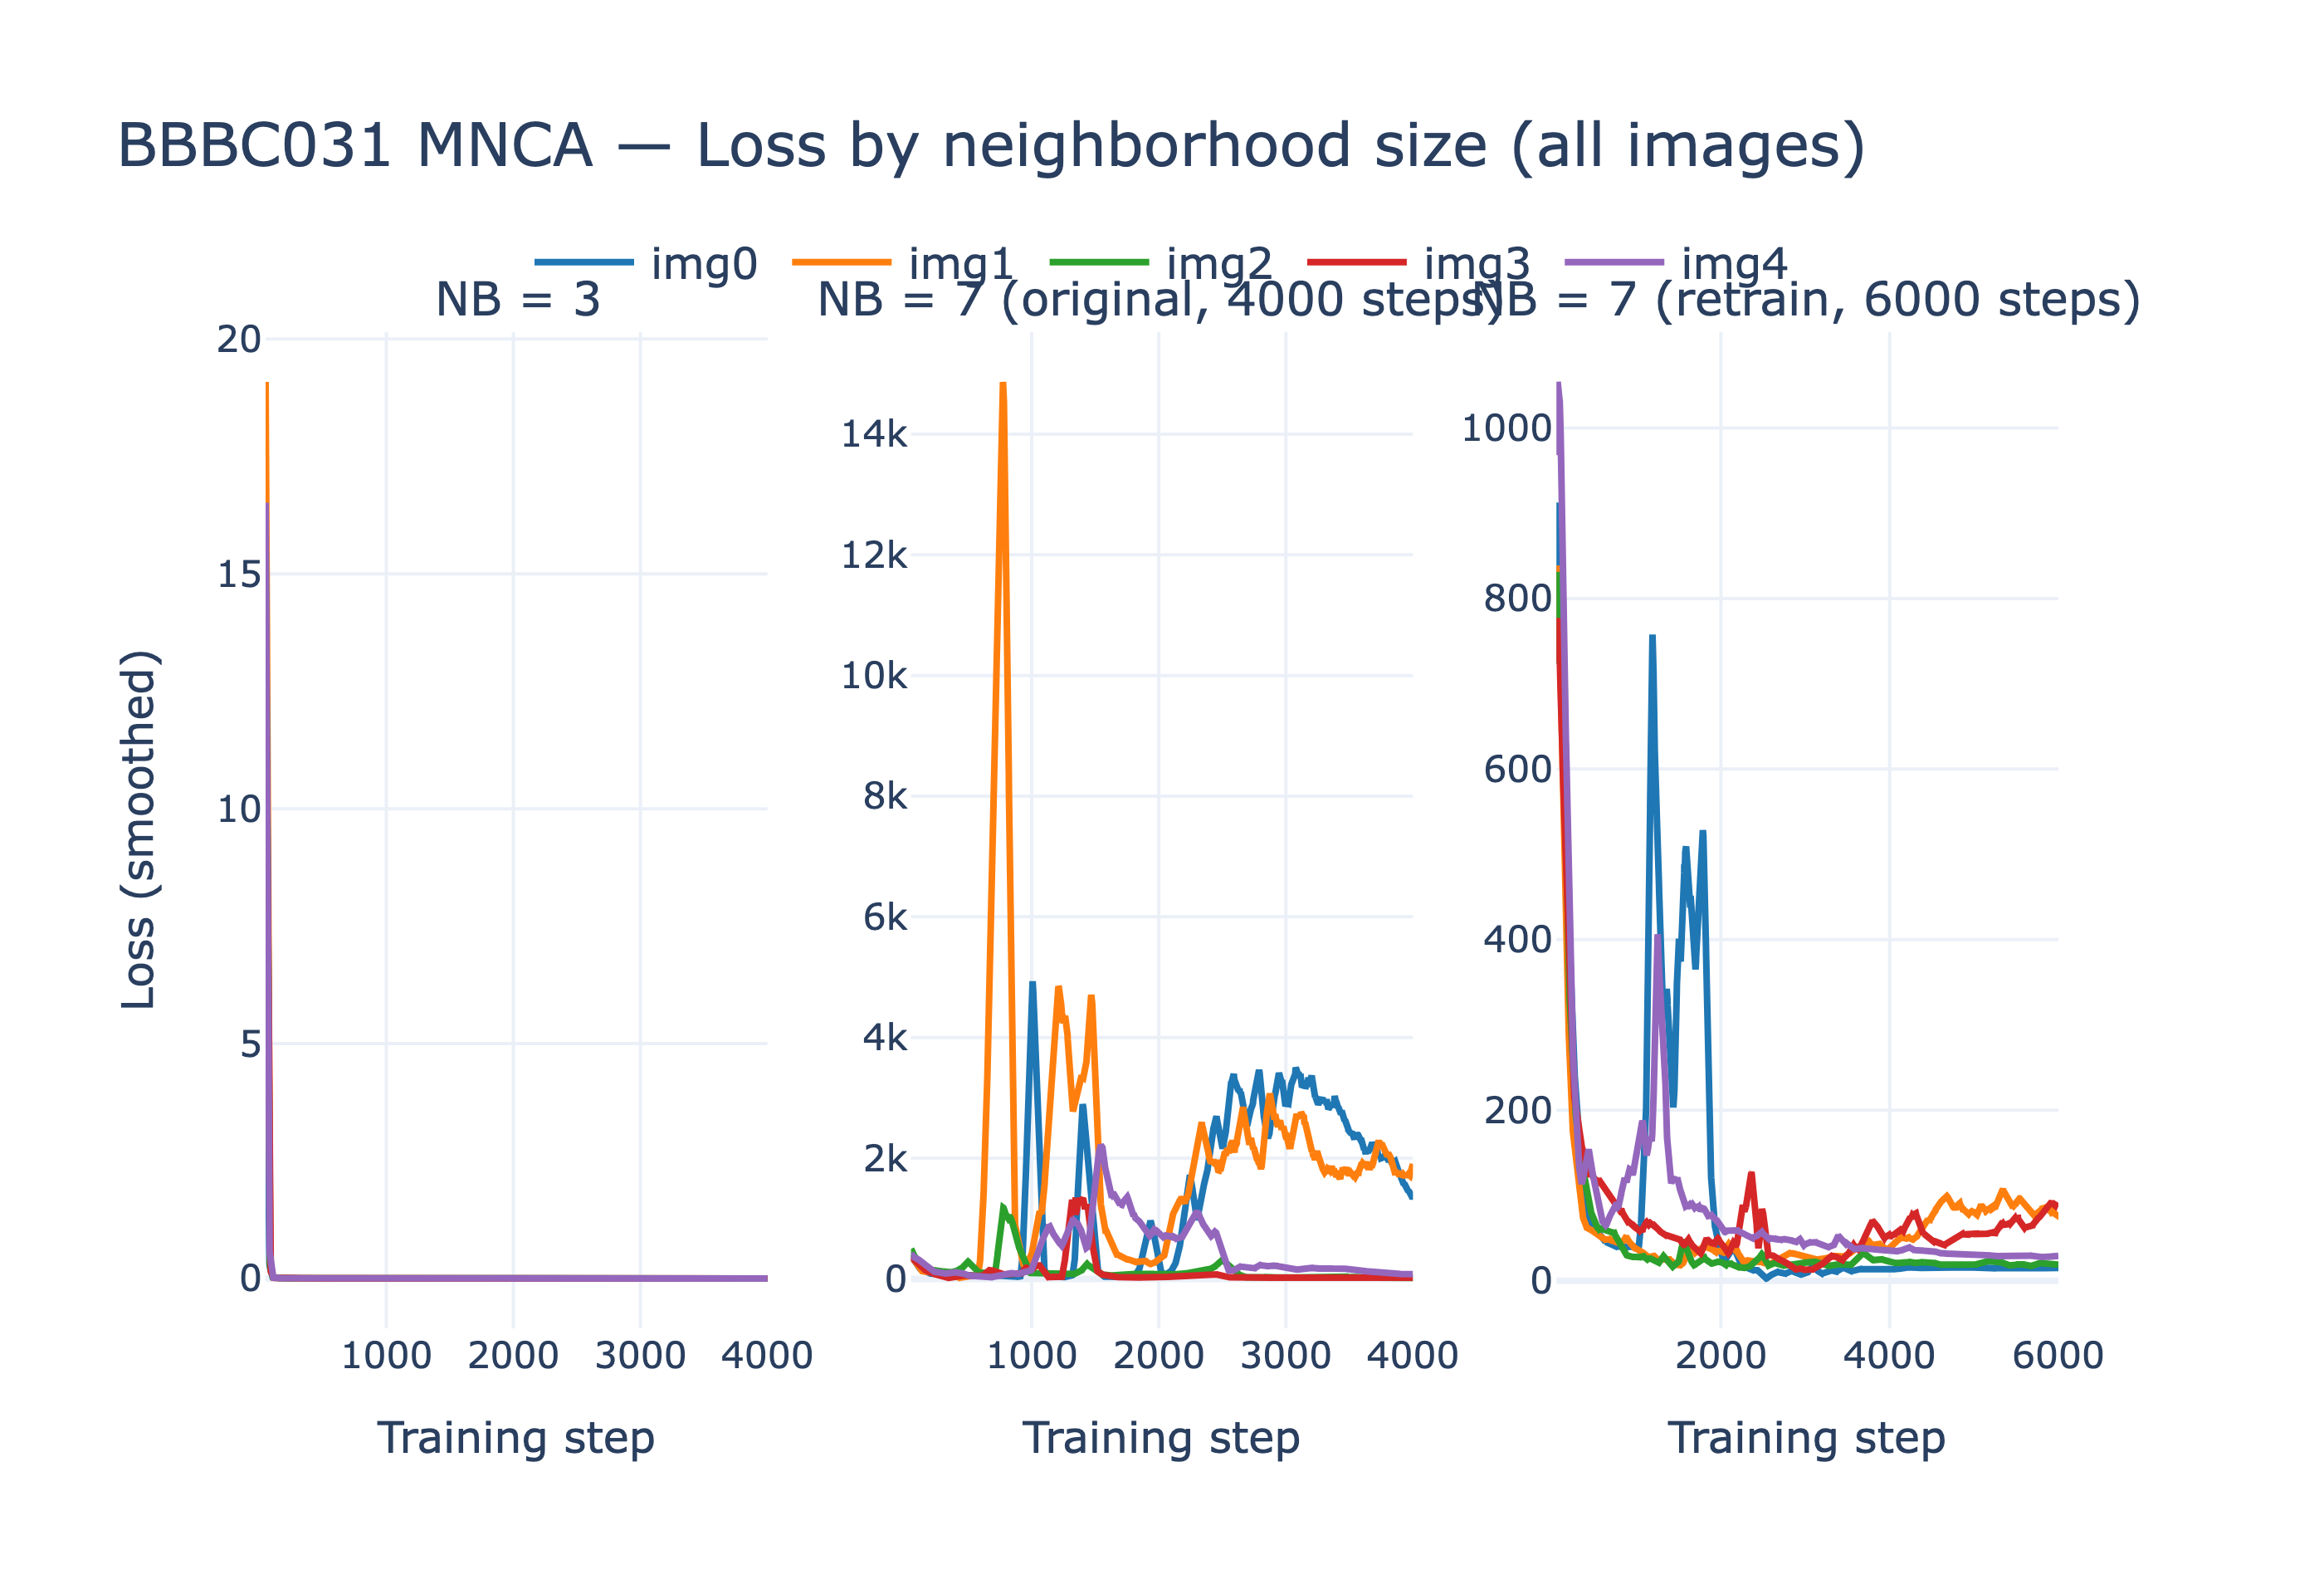
\includegraphics[width=\textwidth]{figs/bbbc031/bbbc031_loss_by_NB.png}
  \caption{BBBC031: loss by neighbourhood size (smoothed). \textbf{Legend:} three panels = \(NB=3\), \(NB=7\) original (4000 steps), \(NB=7\) re-trained (6000 steps); abscissa = training step; ordinate = loss; one curve per image (img0--img4).}
  \label{fig:impl:bbbc031:loss_by_nb}
\end{figure}

\begin{figure}[H]
  \centering
  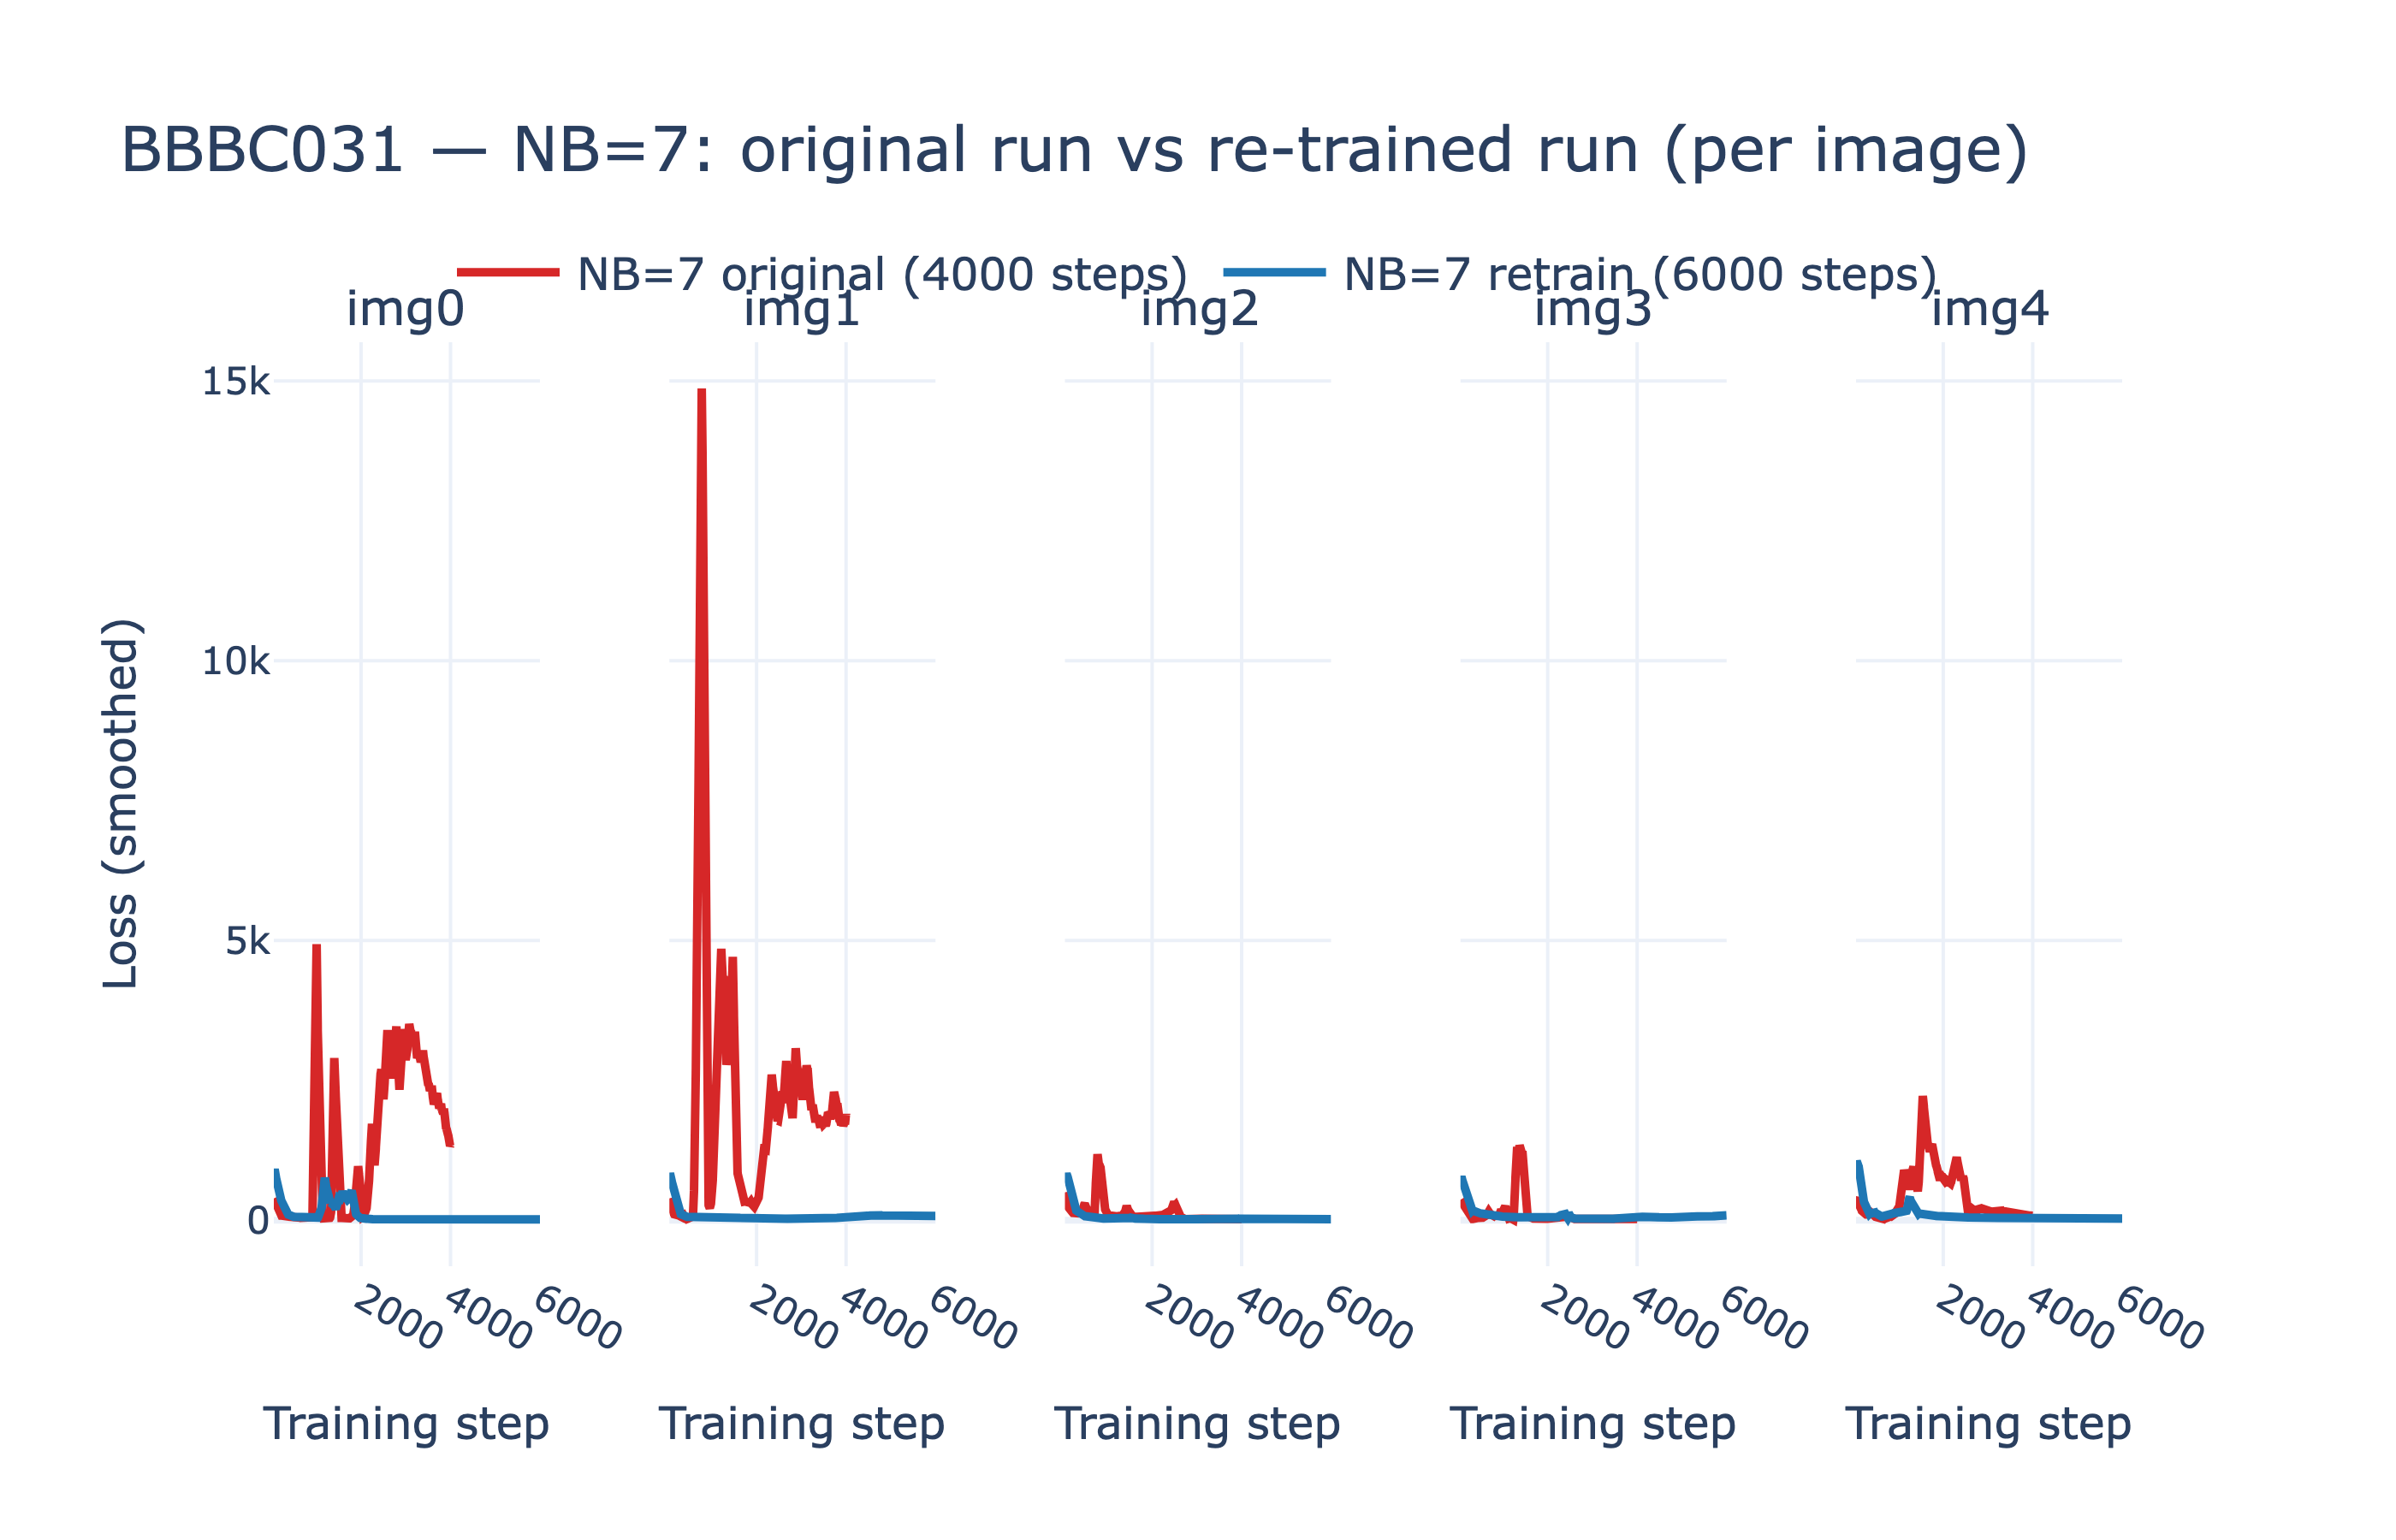
\includegraphics[width=\textwidth]{figs/bbbc031/bbbc031_NB7_original_vs_retrain.png}
  \caption{BBBC031: \(NB=7\) original vs.\ re-trained loss. \textbf{Legend:} one panel per image (img0--img4); abscissa = training step; ordinate = smoothed loss; two curves per panel = original run (4000 steps) and re-trained run (6000 steps).}
  \label{fig:impl:bbbc031:nb7_compare}
\end{figure}

\subsection{Segmentation metrics}

% BBBC031 MNCA metrics table (auto-generated by bbbc031_metrics_thesis.py)
% IoU, Dice, MSE on Stochastic checkpoints NB=3 and NB=7, 20 simulation steps.
% Requires \usepackage{booktabs} in the preamble.
\begin{table}[ht]
\centering
\caption{BBBC031 segmentation metrics: IoU, Dice and MSE (RGBA) per image and neighborhood size (NB).}
\label{tab:bbbc031_metrics}
\begin{tabular}{l|ccc|ccc}
\toprule
Image & \multicolumn{3}{c}{NB=3} & \multicolumn{3}{c}{NB=7} \\
(idx) & IoU & Dice & MSE & IoU & Dice & MSE \\
\midrule
0 & 1.000 & 1.000 & 2.9119e-04 & 0.077 & 0.144 & 3.2822e-01 \\
1 & 0.997 & 0.998 & 1.1005e-03 & 0.171 & 0.292 & 2.9403e-01 \\
2 & 1.000 & 1.000 & 2.8898e-04 & 0.031 & 0.060 & 2.8869e-01 \\
3 & 1.000 & 1.000 & 1.4917e-04 & 0.366 & 0.536 & 3.3028e-01 \\
4 & 0.991 & 0.996 & 2.2697e-03 & 0.056 & 0.107 & 3.0516e-01 \\
\bottomrule
\end{tabular}
\end{table}


\subsubsection{NB=7 original vs.\ re-trained}
\label{sec:impl:bbbc031:retrain}
\vspace{-0.5em}
Re-training \(NB=7\) with a lower learning rate (\(3\times10^{-4}\)) and a longer run (6000 steps) avoids divergence and improves segmentation overlap metrics, although performance remains below the \(NB=3\) reference under the schedules explored.
\vspace{-1.5em}
\paragraph{Comparison of segmentation outputs: \(NB=7\) original vs.\ re-trained.}
Figure~\ref{fig:impl:bbbc031:nb7_output_compare} compares the segmentation outputs (after 20 simulation steps) of the original \(NB=7\) model with the re-trained one, for all five images.
Each row shows, from left to right: ground truth, prediction of the original run (4000 steps, default learning rate), and prediction of the re-trained run (6000 steps, lower learning rate).
\vspace{-0.8em}
\begin{figure}[H]
  \centering
  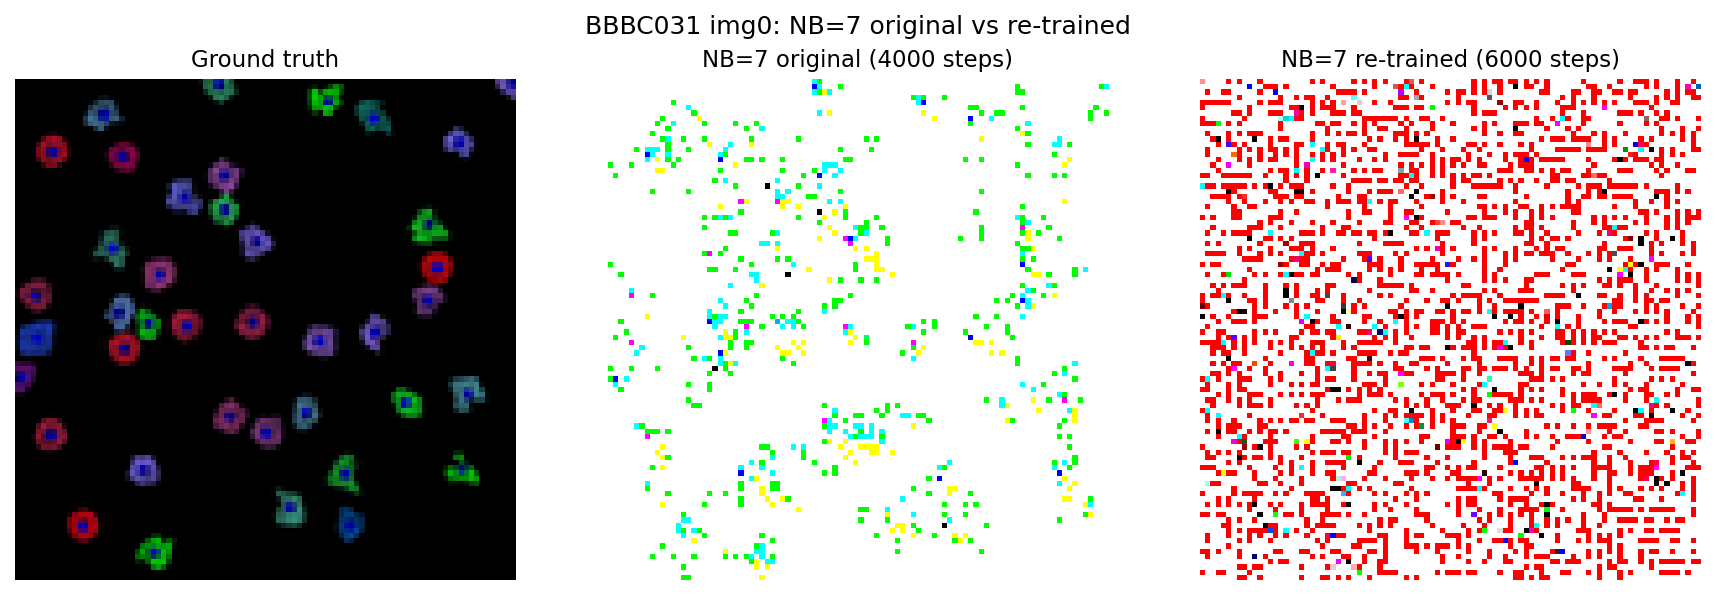
\includegraphics[width=0.98\textwidth]{figs/bbbc031/bbbc031_NB7_original_vs_retrain_img0.png}\\[0.25em]
  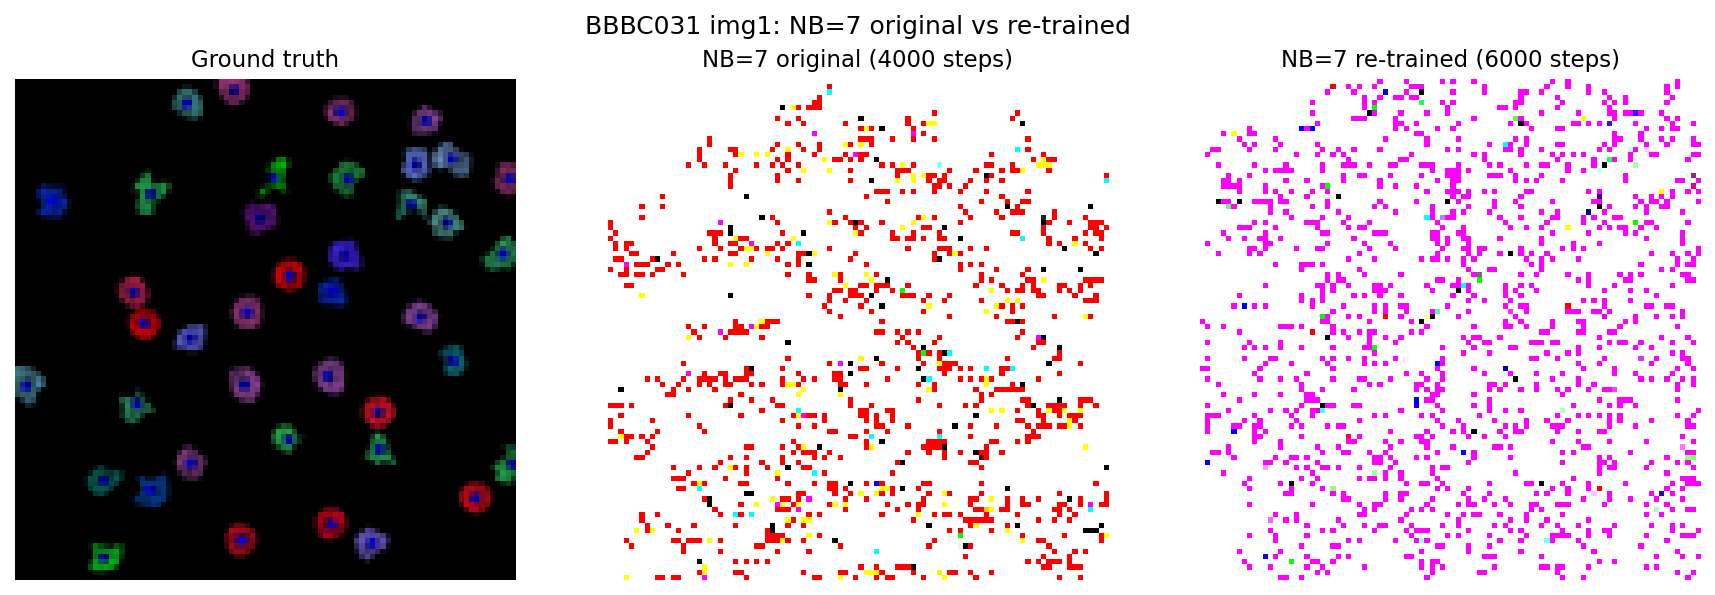
\includegraphics[width=0.98\textwidth]{figs/bbbc031/bbbc031_NB7_original_vs_retrain_img1.png}\\[0.25em]
  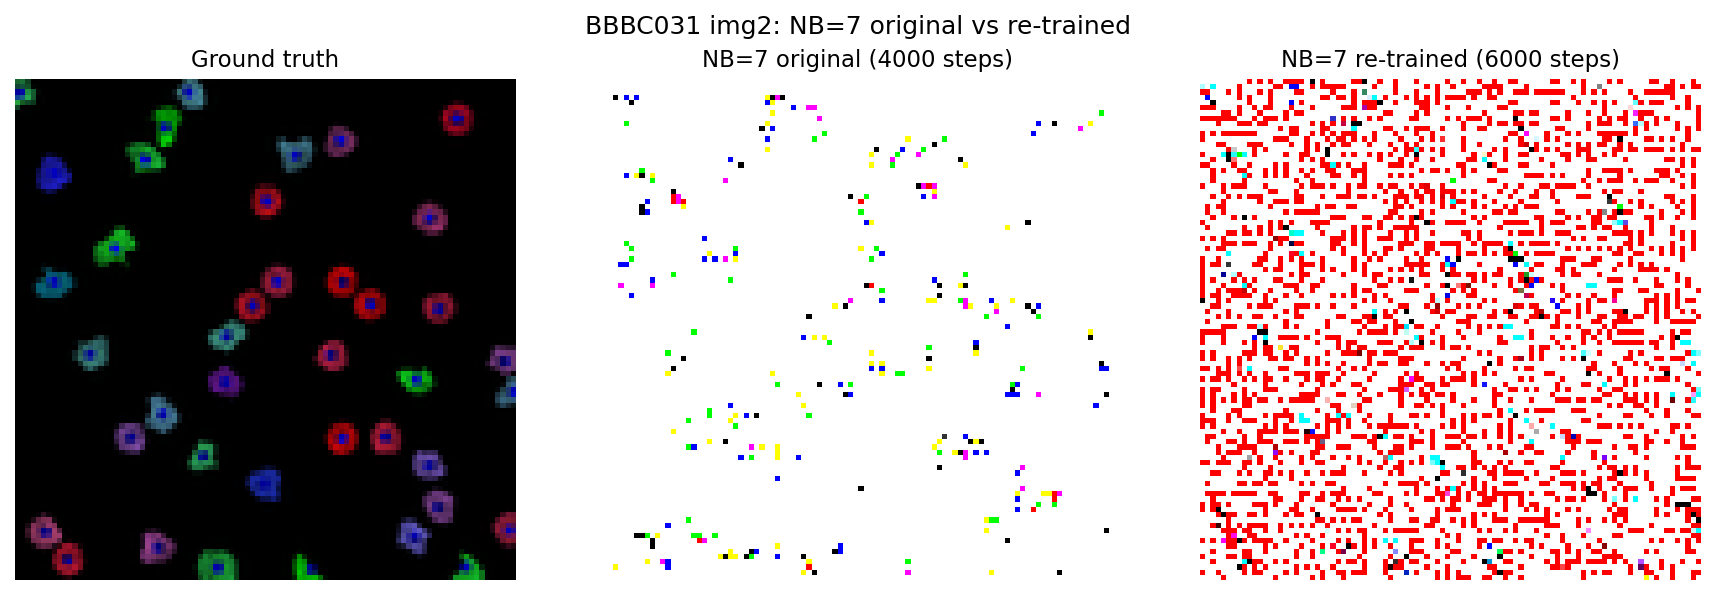
\includegraphics[width=0.98\textwidth]{figs/bbbc031/bbbc031_NB7_original_vs_retrain_img2.png}\\[0.25em]
  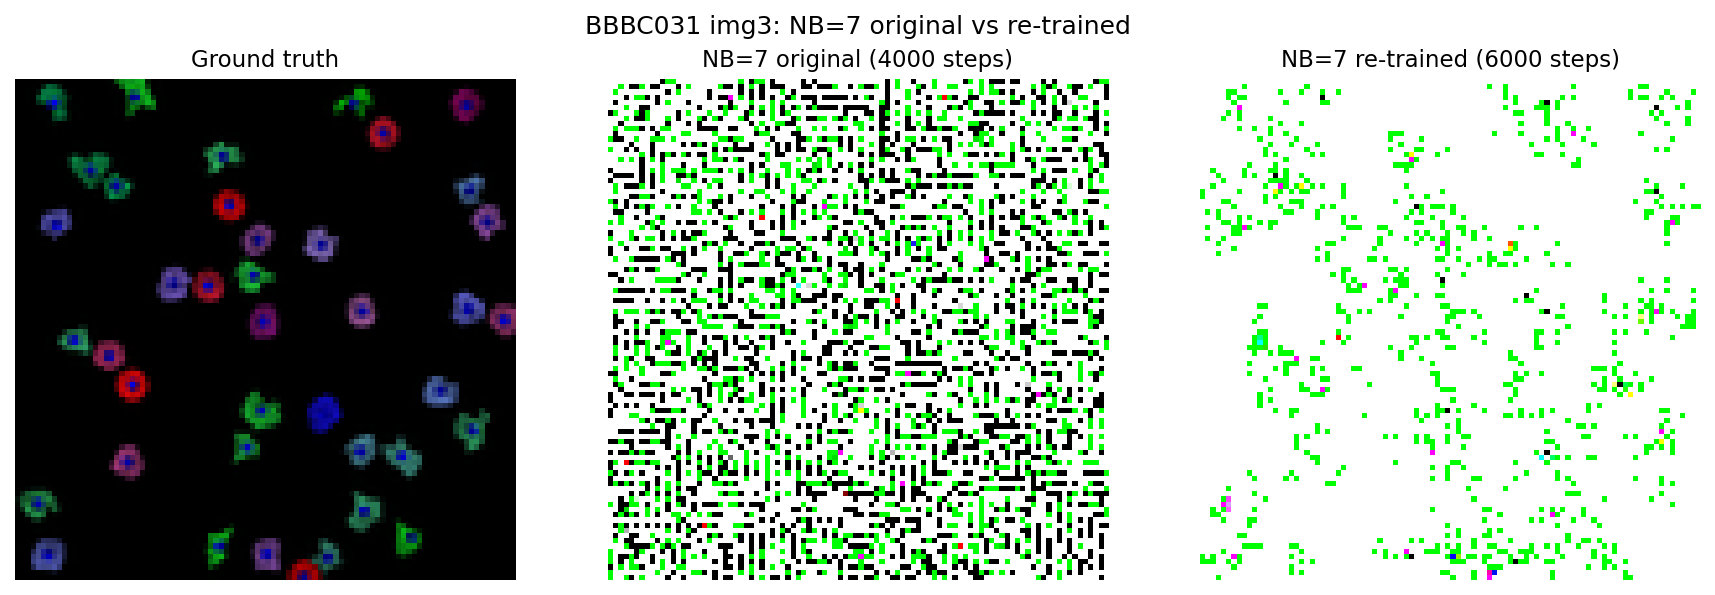
\includegraphics[width=0.98\textwidth]{figs/bbbc031/bbbc031_NB7_original_vs_retrain_img3.png}\\[0.25em]
  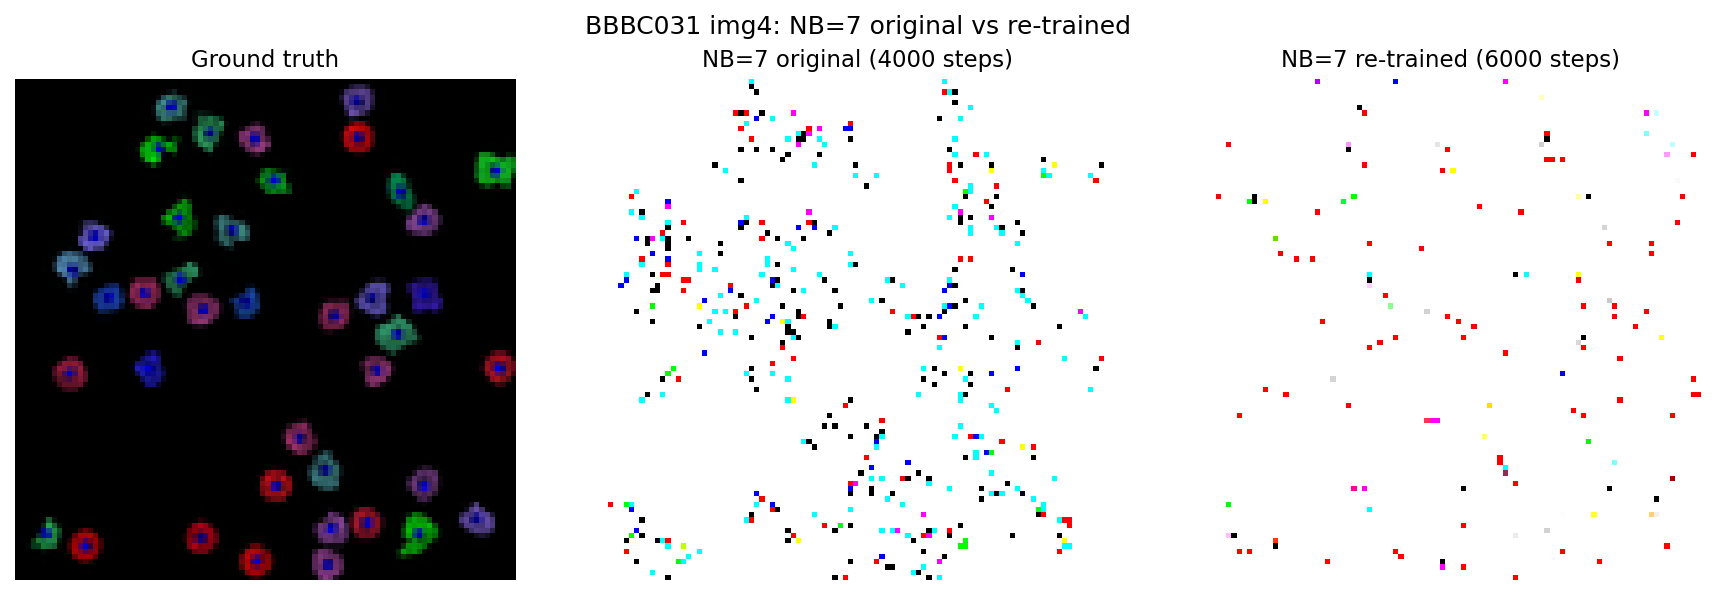
\includegraphics[width=0.98\textwidth]{figs/bbbc031/bbbc031_NB7_original_vs_retrain_img4.png}
  \vspace{0.5em}
  \caption{BBBC031: segmentation outputs for \(NB=7\) after 20 simulation steps. \textbf{Legend:} each row = one image (img0--img4); columns = ground-truth mask, prediction original run (4000 steps), prediction re-trained run (6000 steps).}
  \label{fig:impl:bbbc031:nb7_output_compare}
\end{figure}

\Cref{tab:bbbc031_NB7_comparison} reports the same comparison in terms of IoU, Dice, and MSE.

% NB=7 original vs re-trained metrics (auto-generated)
% IoU/Dice on alpha mask; MSE on RGBA; MSE_RGB on RGB only (colour fidelity).
% Requires \usepackage{booktabs} in the preamble.
\begin{table}[H]
\centering
\caption{BBBC031: comparison between NB=7 original (4000 steps, LR $10^{-3}$) and re-trained (6000 steps, LR $3\times10^{-4}$). IoU and Dice use the alpha channel; MSE is on all RGBA channels; MSE\_RGB is on RGB only (colour fidelity).}
\label{tab:bbbc031_NB7_comparison}
\vspace{0.5em}
\resizebox{\textwidth}{!}{%
\begin{tabular}{c|cccc|cccc|cccc}
\toprule
Image & \multicolumn{4}{c}{NB=7 original} & \multicolumn{4}{c}{NB=7 re-trained} & \multicolumn{4}{c}{$\Delta$ (retrain $-$ orig)} \\
(idx) & IoU & Dice & MSE & MSE\_RGB & IoU & Dice & MSE & MSE\_RGB & IoU & Dice & MSE & MSE\_RGB \\
\midrule
0 & 0.095 & 0.174 & 3.3991e-01 & 1.5170e-01 & 0.301 & 0.463 & 3.5285e-01 & 2.3784e-01 & +0.206 & +0.289 & +1.2947e-02 & +8.6140e-02 \\
1 & 0.179 & 0.304 & 2.9670e-01 & 1.2212e-01 & 0.372 & 0.543 & 4.0718e-01 & 3.3381e-01 & +0.193 & +0.238 & +1.1048e-01 & +2.1169e-01 \\
2 & 0.030 & 0.058 & 2.8579e-01 & 5.7618e-02 & 0.291 & 0.451 & 3.6456e-01 & 2.4996e-01 & +0.261 & +0.393 & +7.8779e-02 & +1.9235e-01 \\
3 & 0.361 & 0.531 & 3.3476e-01 & 2.3358e-01 & 0.099 & 0.180 & 3.3511e-01 & 1.4645e-01 & -0.263 & -0.351 & +3.5074e-04 & -8.7135e-02 \\
4 & 0.060 & 0.113 & 3.0988e-01 & 9.9813e-02 & 0.408 & 0.580 & 4.3196e-01 & 3.7886e-01 & +0.349 & +0.467 & +1.2208e-01 & +2.7904e-01 \\
\bottomrule
\end{tabular}%
}
\end{table}


\subsubsection{Qualitative examples: seeds, \(NB=3\), and \(NB=7\)}

\begin{figure}[H]
  \centering
  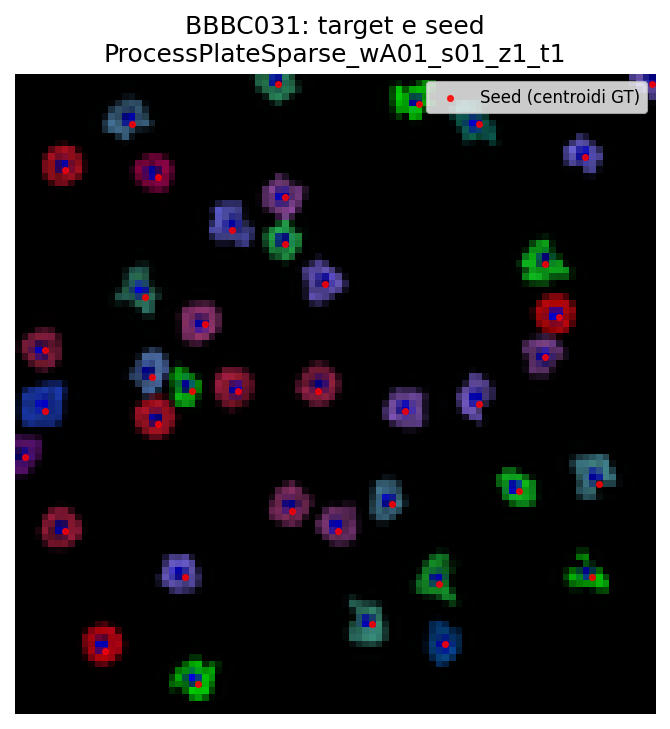
\includegraphics[width=0.7\textwidth]{figs/bbbc031/bbbc031_target_and_seed.png}
  \caption{BBBC031: ground-truth cell mask and seed points. \textbf{Legend:} mask = ground-truth segmentation (CELLMASK); points = cell centroids (seeds); the NCA is initialised from these seeds and run for 20 steps.}
  \label{fig:impl:bbbc031:target_seed}
\end{figure}

\begin{figure}[H]
  \centering
  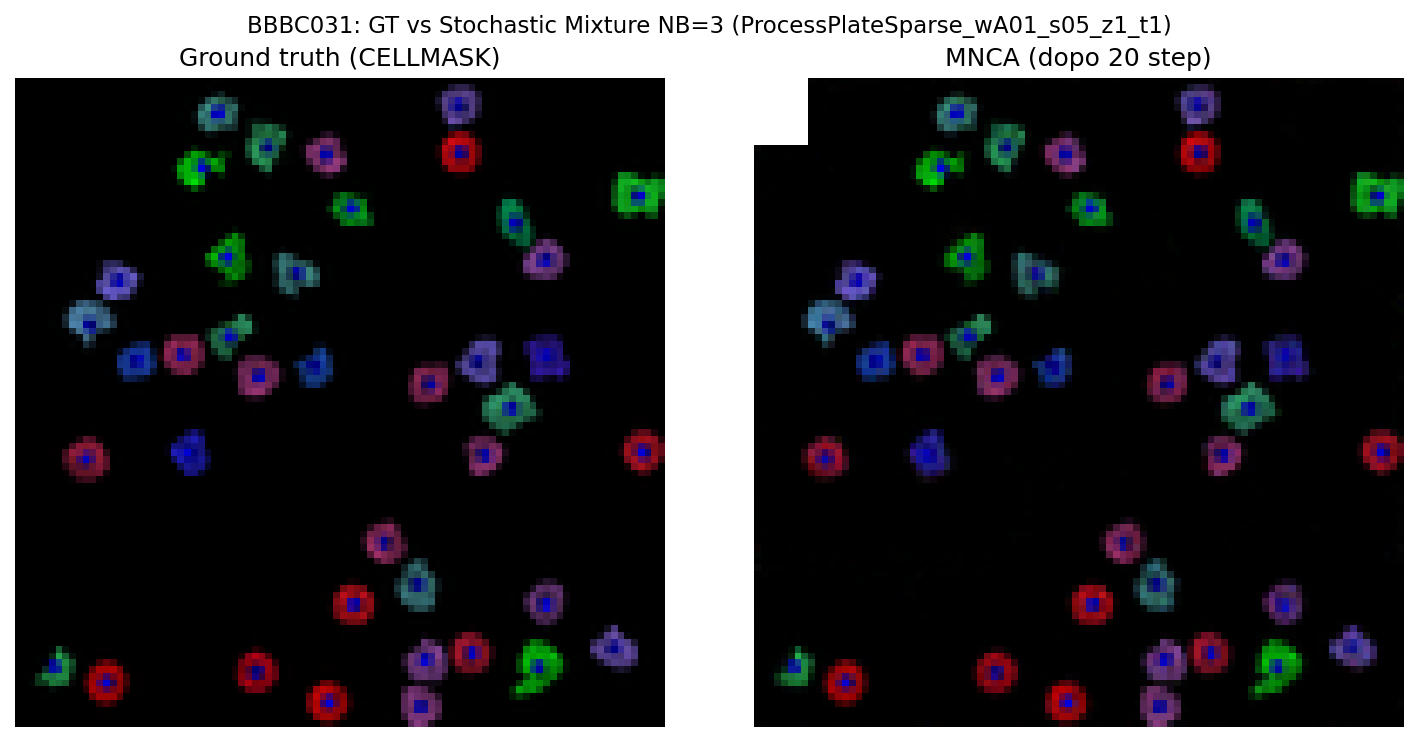
\includegraphics[width=\textwidth]{figs/bbbc031/bbbc031_gt_vs_mnca_trained_here_NB3_stochastic.png}
  \caption{BBBC031: ground truth vs.\ prediction, \(NB=3\). \textbf{Legend:} left = ground-truth mask; right = Stochastic Mixture NCA output after 20 steps.}
  \label{fig:impl:bbbc031:gt_vs_nb3}
\end{figure}

\begin{figure}[H]
  \centering
  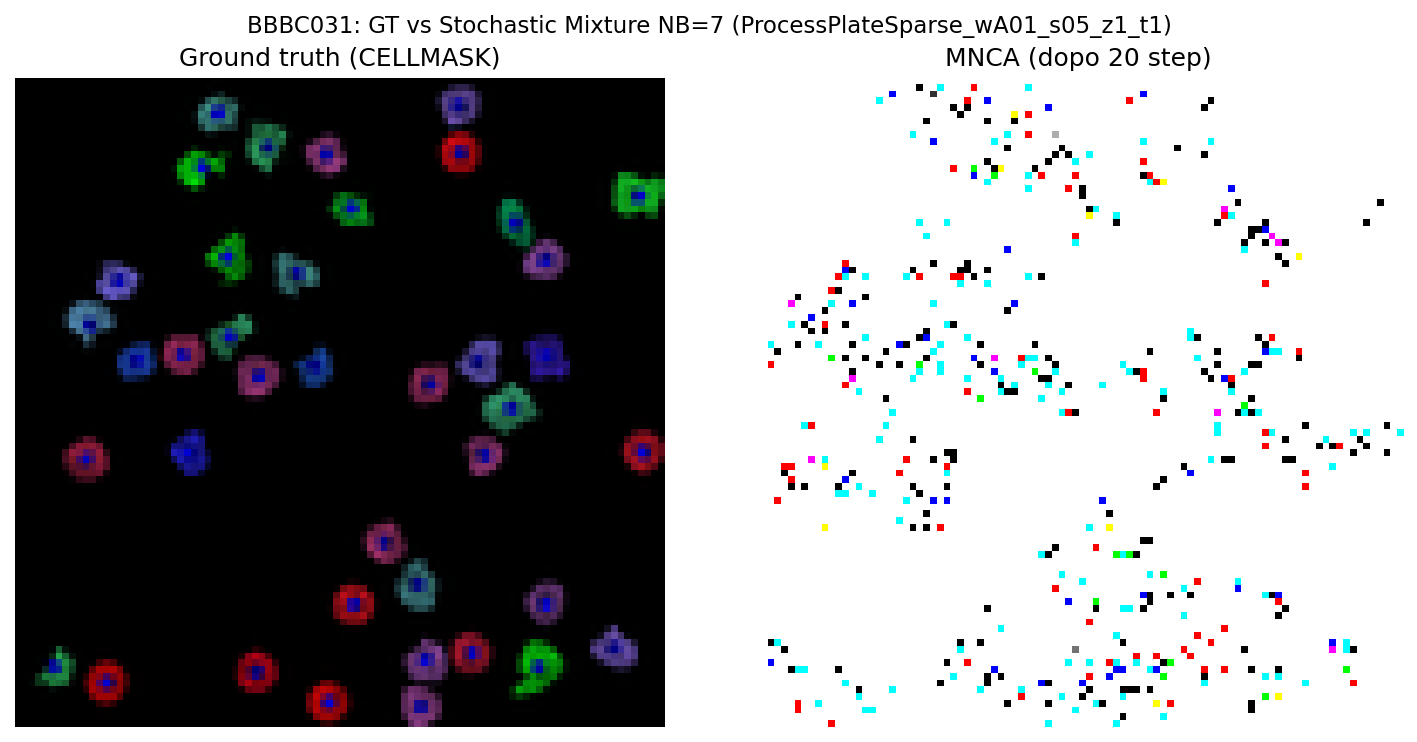
\includegraphics[width=\textwidth]{figs/bbbc031/bbbc031_gt_vs_mnca_trained_here_NB7_stochastic.png}
  \caption{BBBC031: ground truth vs.\ prediction, \(NB=7\) original run. \textbf{Legend:} left = ground-truth mask; right = Stochastic Mixture NCA (\(NB=7\), 4000 steps) after 20 simulation steps.}
  \label{fig:impl:bbbc031:gt_vs_nb7}
\end{figure}

\begin{figure}[H]
  \centering
  \begin{minipage}[t]{0.32\textwidth}
    \centering
    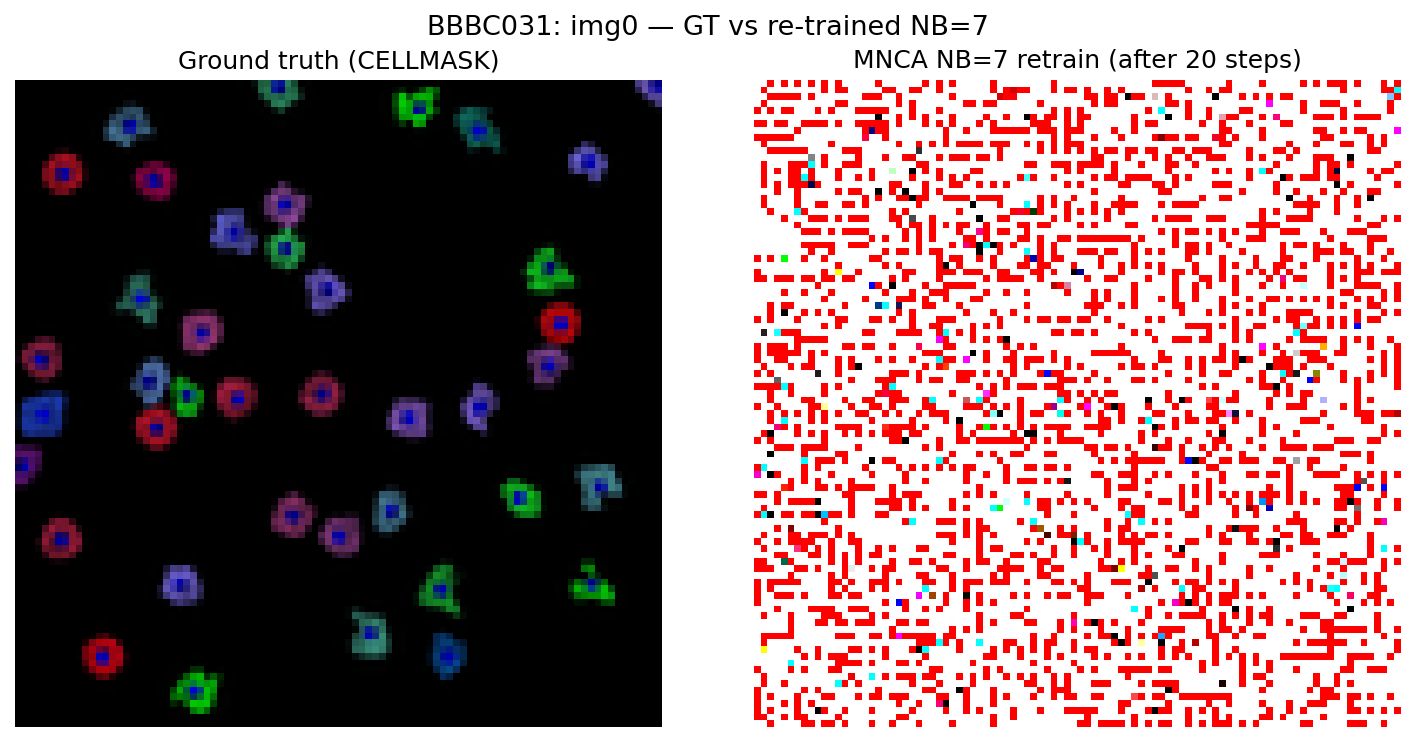
\includegraphics[width=\textwidth]{figs/bbbc031/bbbc031_gt_vs_mnca_NB7_retrain_img0.png}
    \caption*{img0}
  \end{minipage}\hfill
  \begin{minipage}[t]{0.32\textwidth}
    \centering
    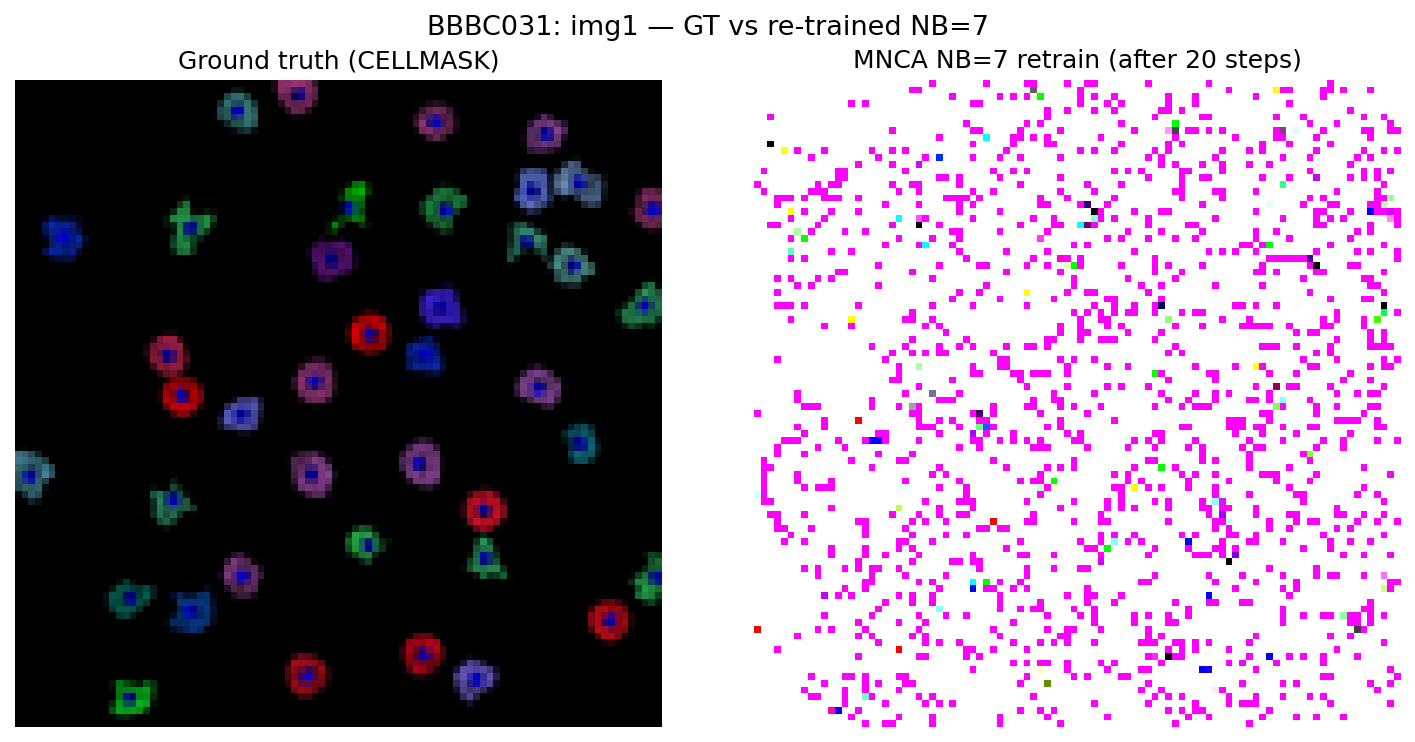
\includegraphics[width=\textwidth]{figs/bbbc031/bbbc031_gt_vs_mnca_NB7_retrain_img1.png}
    \caption*{img1}
  \end{minipage}\hfill
  \begin{minipage}[t]{0.32\textwidth}
    \centering
    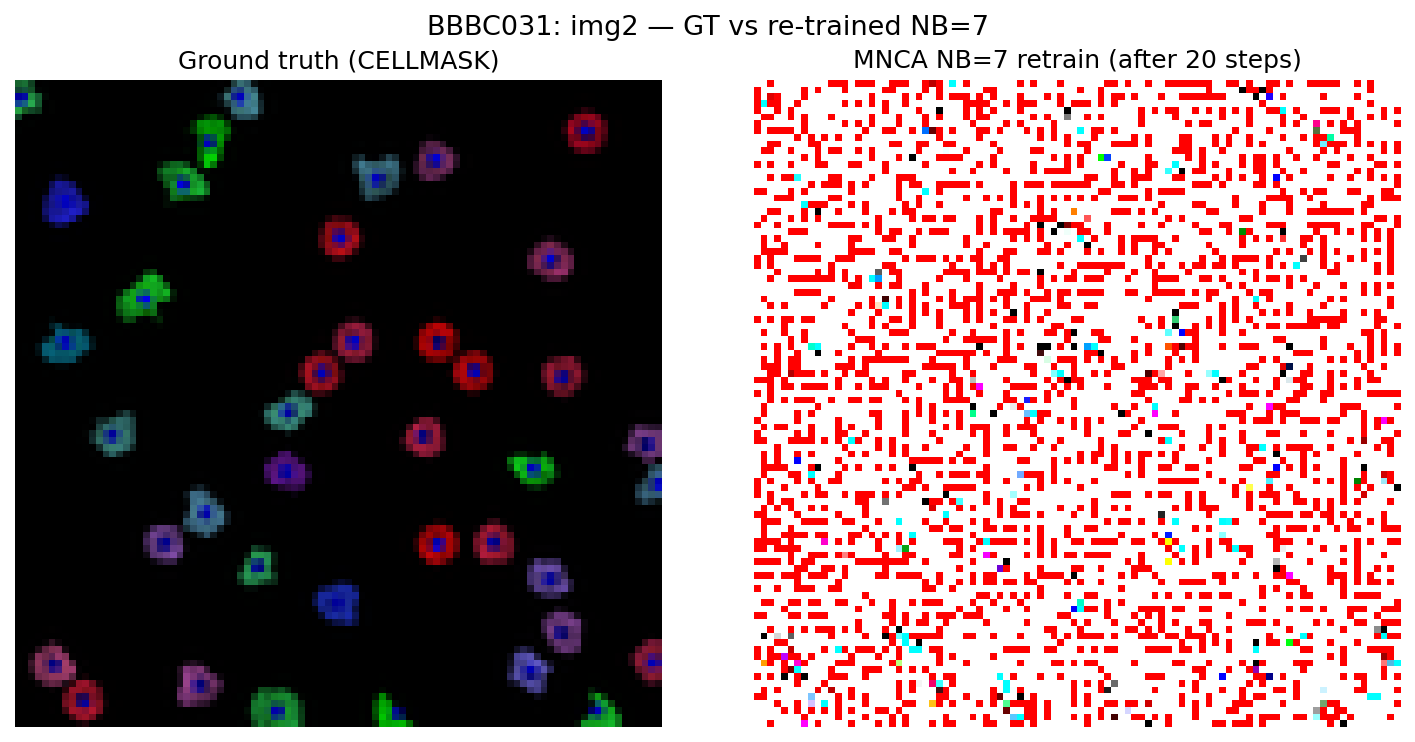
\includegraphics[width=\textwidth]{figs/bbbc031/bbbc031_gt_vs_mnca_NB7_retrain_img2.png}
    \caption*{img2}
  \end{minipage}\\[0.5em]
  \hfill
  \begin{minipage}[t]{0.32\textwidth}
    \centering
    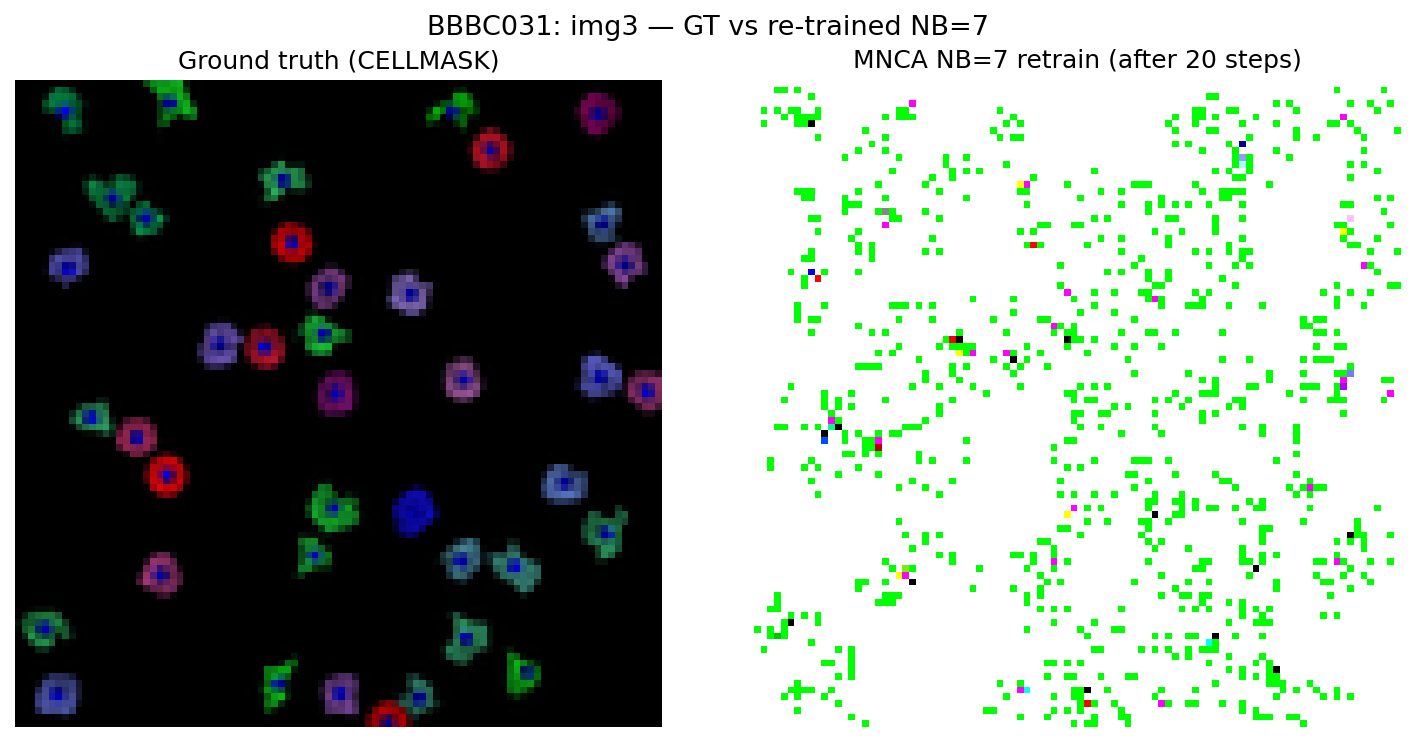
\includegraphics[width=\textwidth]{figs/bbbc031/bbbc031_gt_vs_mnca_NB7_retrain_img3.png}
    \caption*{img3}
  \end{minipage}\hfill
  \begin{minipage}[t]{0.32\textwidth}
    \centering
    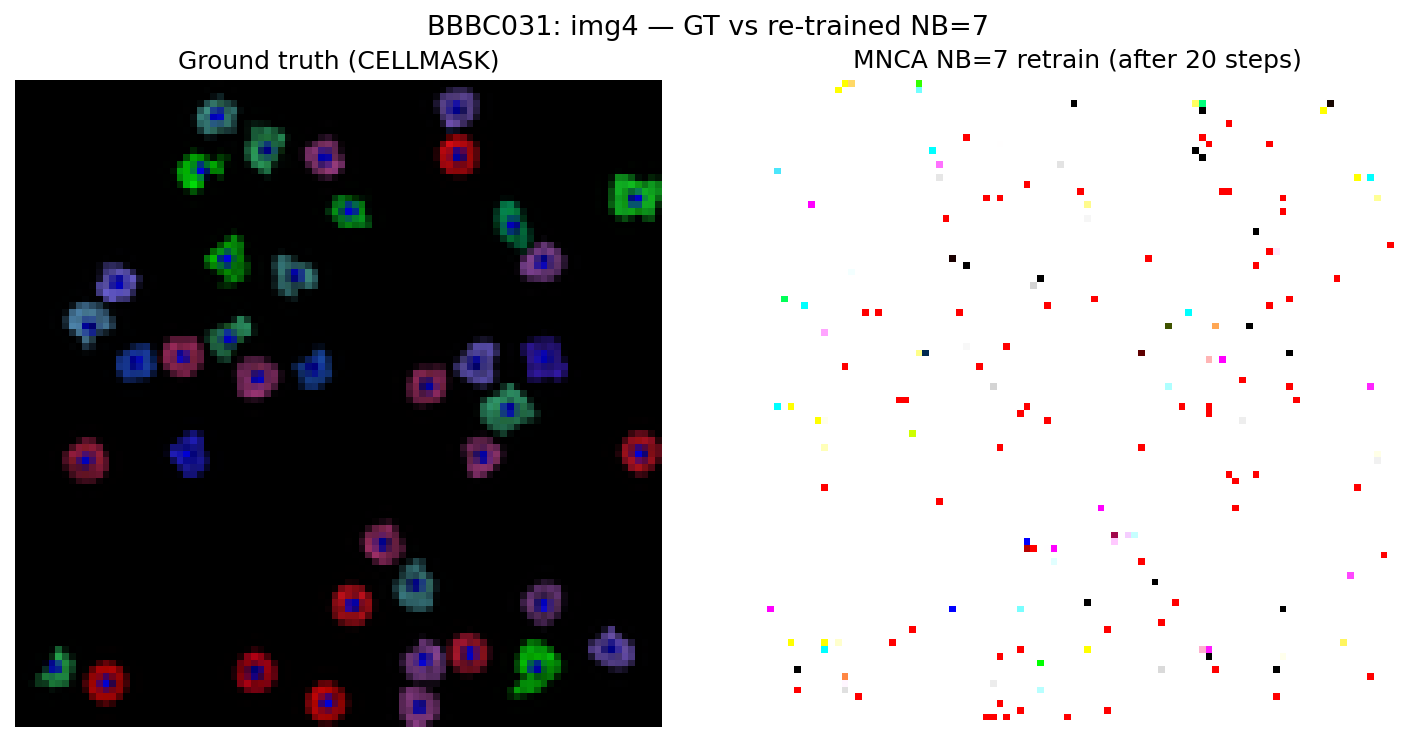
\includegraphics[width=\textwidth]{figs/bbbc031/bbbc031_gt_vs_mnca_NB7_retrain_img4.png}
    \caption*{img4}
  \end{minipage}\hfill
  \caption{BBBC031: outputs from re-trained \(NB=7\) (20 steps). \textbf{Legend:} five panels = img0--img4; each panel = ground truth (left) vs.\ prediction (right).}
  \label{fig:impl:bbbc031:gt_vs_nb7_retrain}
\end{figure}

\subsubsection{Extended re-training at 12\,000 steps}
\label{sec:impl:bbbc031:retrain12k}

To test whether a longer optimisation and a finer learning-rate schedule could reduce the remaining gap for \(NB=7\), we ran an extended re-training at 12\,000 steps (same learning rate as the 6000-step re-training, but with four milestones).

% NB=7 6000 vs 12000 steps metrics (auto-generated)
% Requires \usepackage{booktabs} in the preamble.
\begin{table}[H]
\centering
\caption{BBBC031: segmentation metrics for NB=7 re-trained run at 6000 steps vs extended run at 12000 steps (LR $3\times10^{-4}$, milestones at 4500, 6000, 7500, 9500).}
\label{tab:bbbc031_NB7_6k_vs_12k}
\vspace{0.5em}
\begin{tabular}{c|ccc|ccc|ccc}
\toprule
Image & \multicolumn{3}{c}{6k steps} & \multicolumn{3}{c}{12k steps} & \multicolumn{3}{c}{$\Delta$ (12k $-$ 6k)} \\
(idx) & IoU & Dice & MSE & IoU & Dice & MSE & IoU & Dice & MSE \\
\midrule
0 & 0.299 & 0.460 & 3.5363e-01 & 0.330 & 0.496 & 4.2480e-01 & +0.031 & +0.036 & +7.1169e-02 \\
1 & 0.373 & 0.544 & 4.0621e-01 & 0.420 & 0.592 & 3.3443e-01 & +0.047 & +0.048 & -7.1774e-02 \\
2 & 0.288 & 0.447 & 3.6465e-01 & 0.483 & 0.651 & 4.4987e-01 & +0.195 & +0.204 & +8.5217e-02 \\
3 & 0.089 & 0.163 & 3.2662e-01 & 0.424 & 0.595 & 4.3512e-01 & +0.335 & +0.432 & +1.0850e-01 \\
4 & 0.405 & 0.576 & 4.3086e-01 & 0.991 & 0.996 & 2.4332e-01 & +0.586 & +0.419 & -1.8754e-01 \\
\bottomrule
\end{tabular}
\end{table}


\begin{figure}[H]
  \centering
  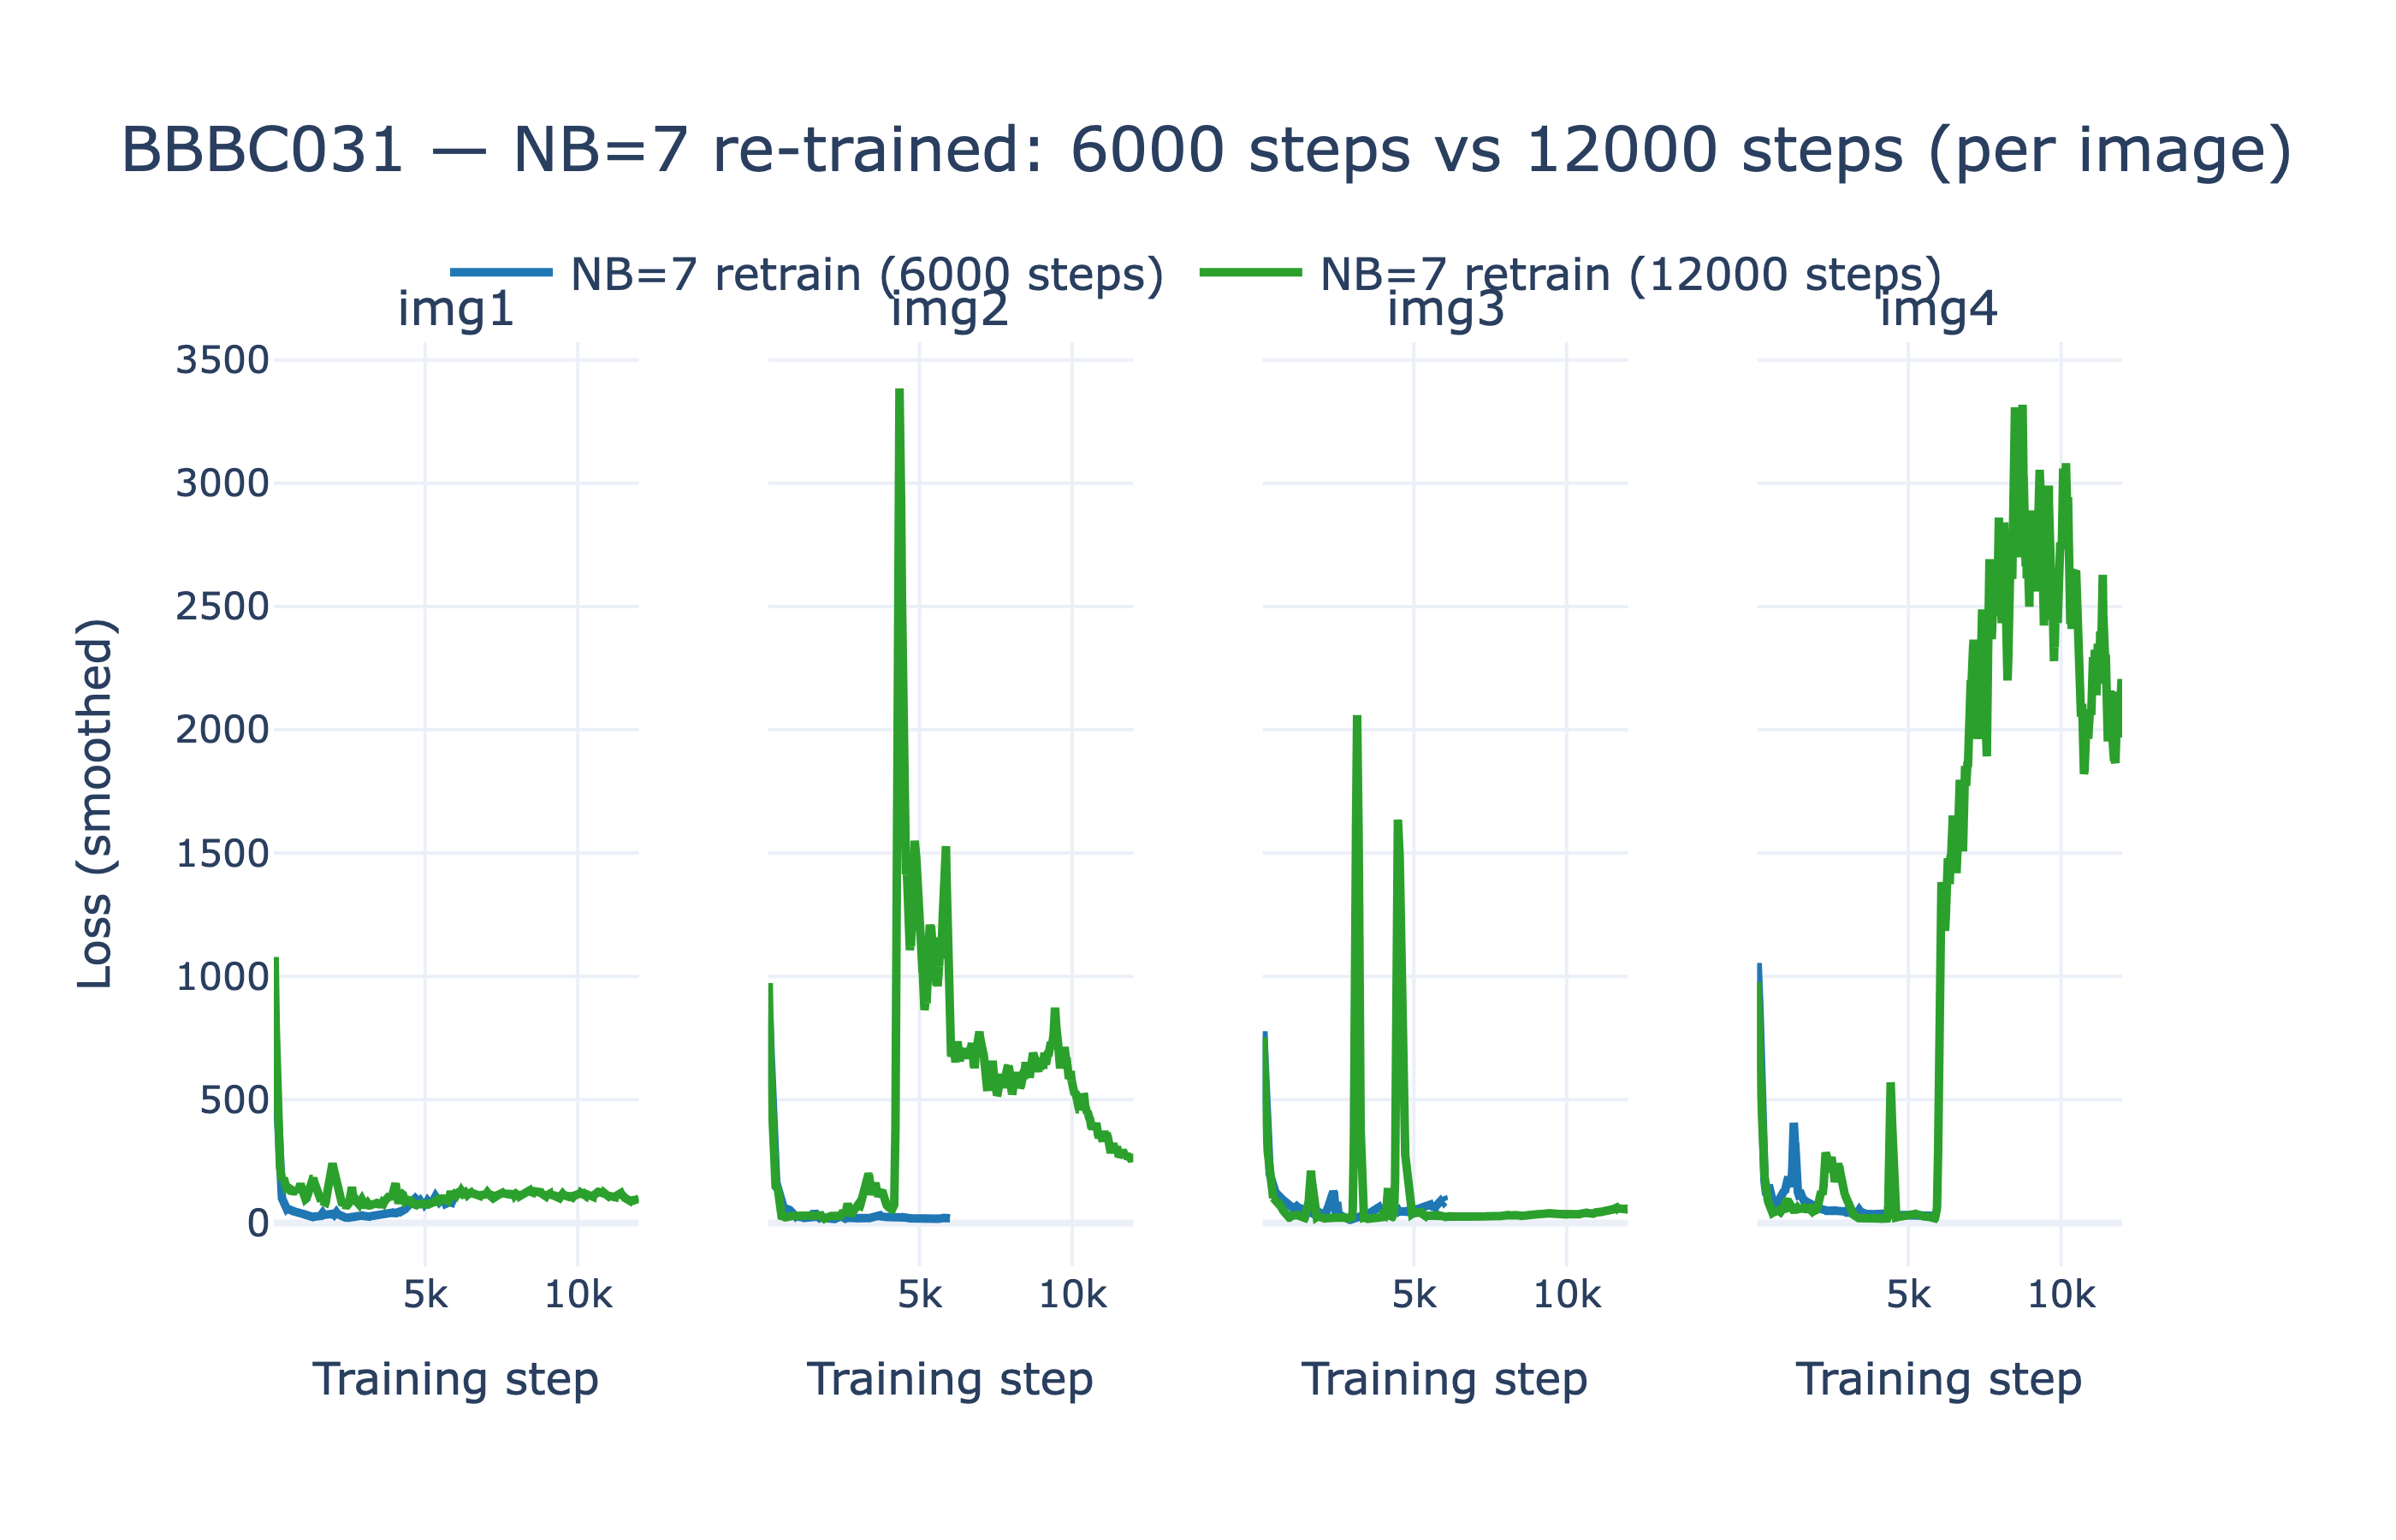
\includegraphics[width=\textwidth]{figs/bbbc031/bbbc031_NB7_6k_vs_12k.png}
  \caption{BBBC031: \(NB=7\) re-trained at 6000 vs.\ 12\,000 steps. \textbf{Legend:} one panel per image (img0--img4); abscissa = training step; ordinate = loss; two curves = 6k run and 12k run (same learning rate, four milestones for 12k).}
  \label{fig:impl:bbbc031:nb7_6k_vs_12k_loss}
\end{figure}

\begin{figure}[H]
  \centering
  \begin{minipage}[t]{0.32\textwidth}
    \centering
    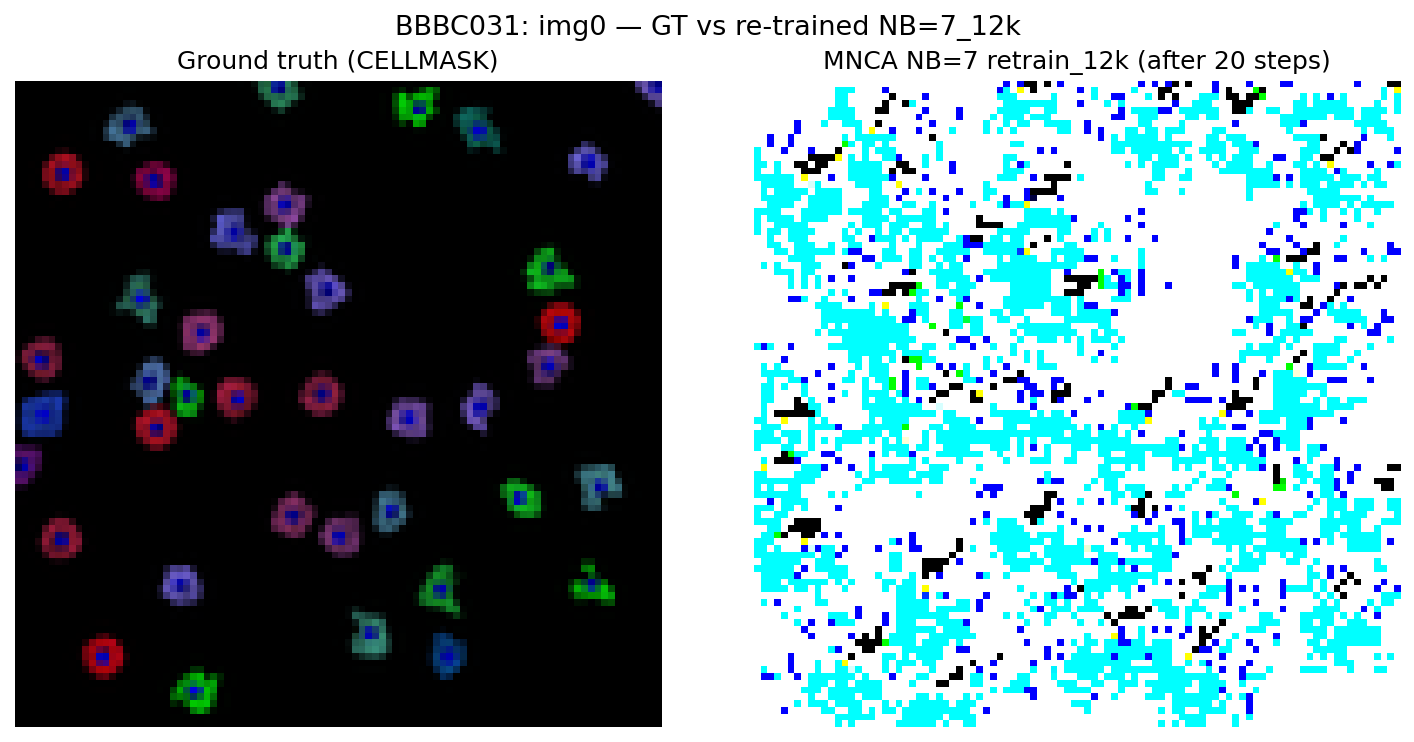
\includegraphics[width=\textwidth]{figs/bbbc031/bbbc031_gt_vs_mnca_NB7_retrain_12k_img0.png}
    \caption*{img0}
  \end{minipage}\hfill
  \begin{minipage}[t]{0.32\textwidth}
    \centering
    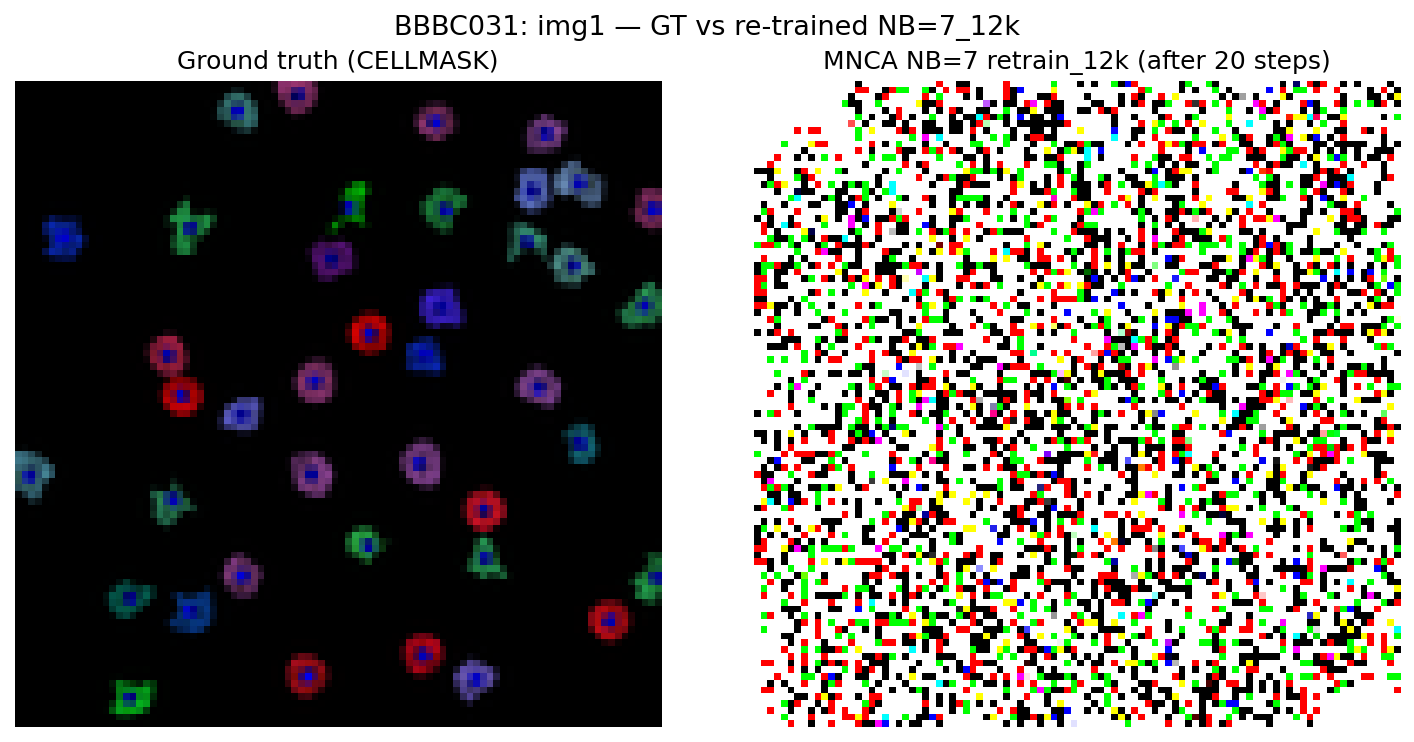
\includegraphics[width=\textwidth]{figs/bbbc031/bbbc031_gt_vs_mnca_NB7_retrain_12k_img1.png}
    \caption*{img1}
  \end{minipage}\hfill
  \begin{minipage}[t]{0.32\textwidth}
    \centering
    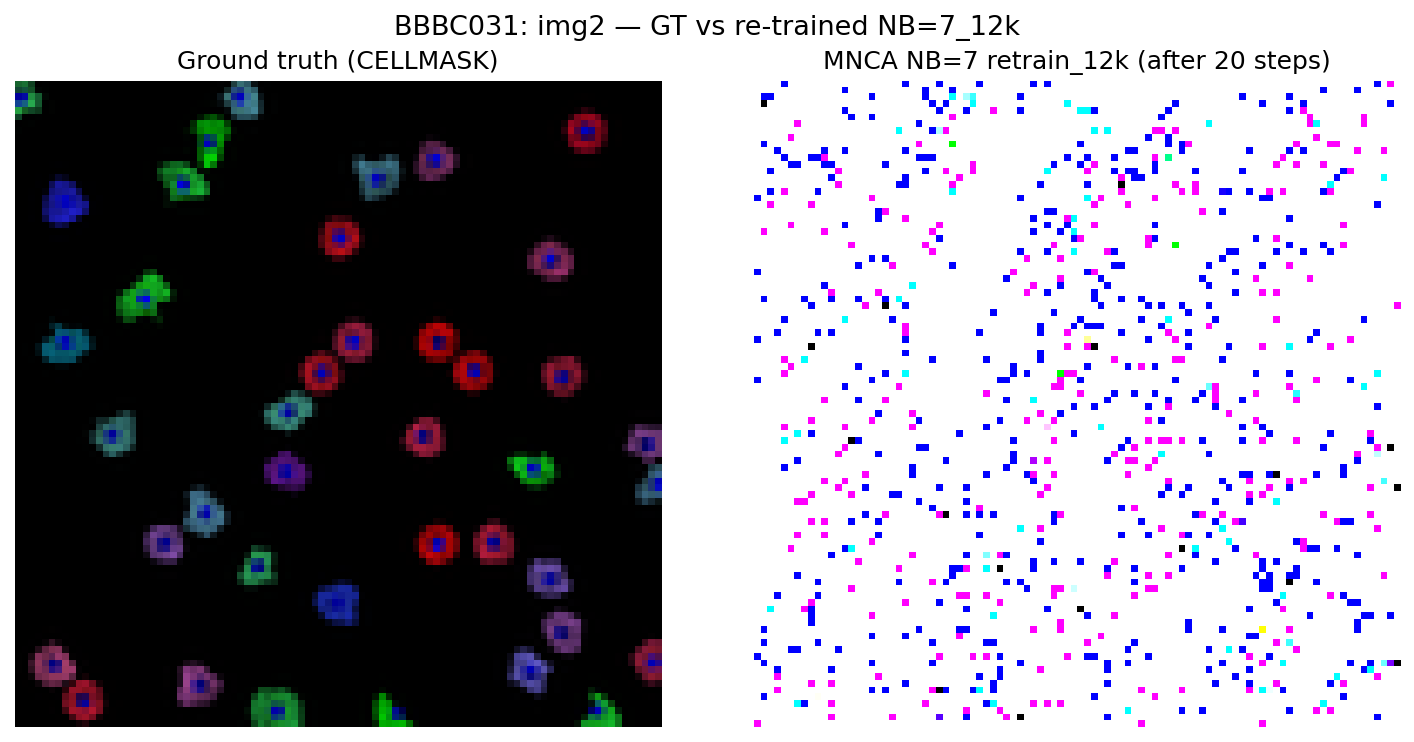
\includegraphics[width=\textwidth]{figs/bbbc031/bbbc031_gt_vs_mnca_NB7_retrain_12k_img2.png}
    \caption*{img2}
  \end{minipage}\\[0.5em]
  \hfill
  \begin{minipage}[t]{0.32\textwidth}
    \centering
    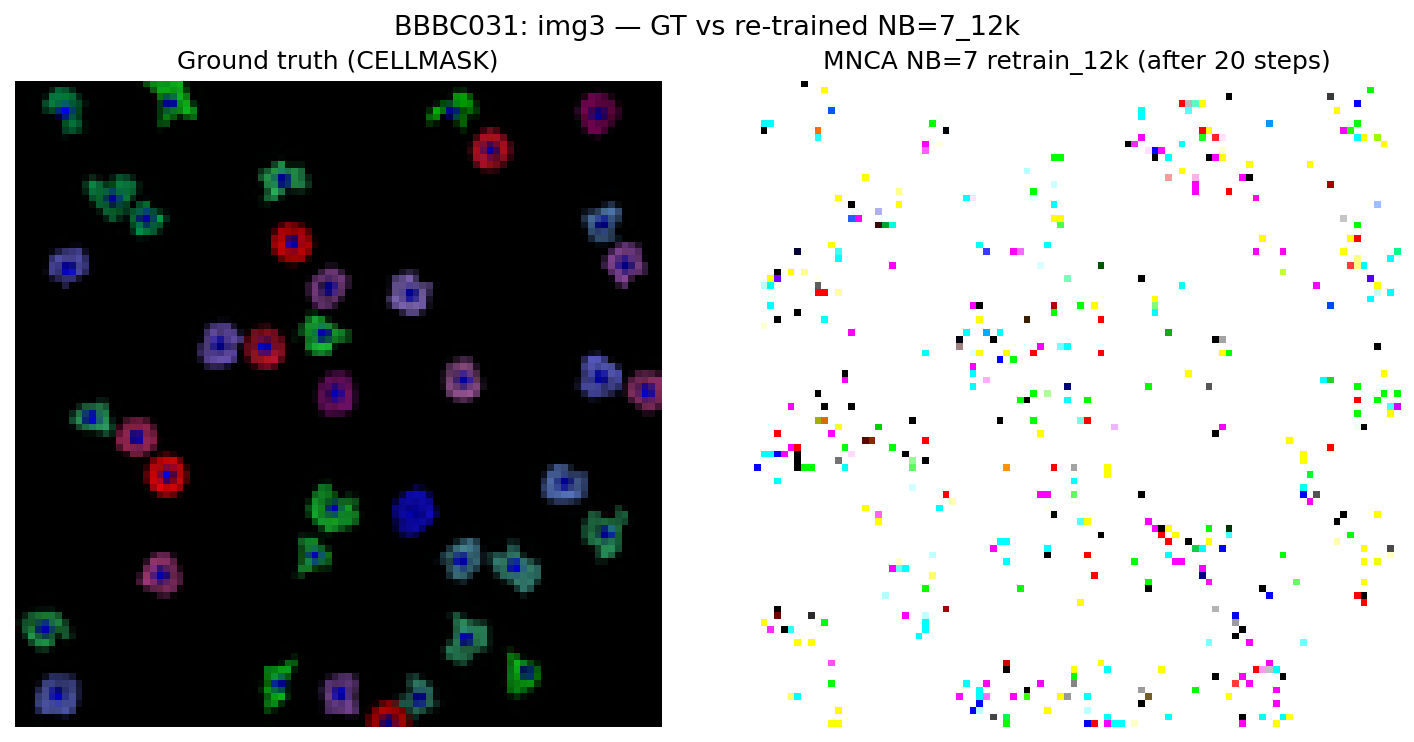
\includegraphics[width=\textwidth]{figs/bbbc031/bbbc031_gt_vs_mnca_NB7_retrain_12k_img3.png}
    \caption*{img3}
  \end{minipage}\hfill
  \begin{minipage}[t]{0.32\textwidth}
    \centering
    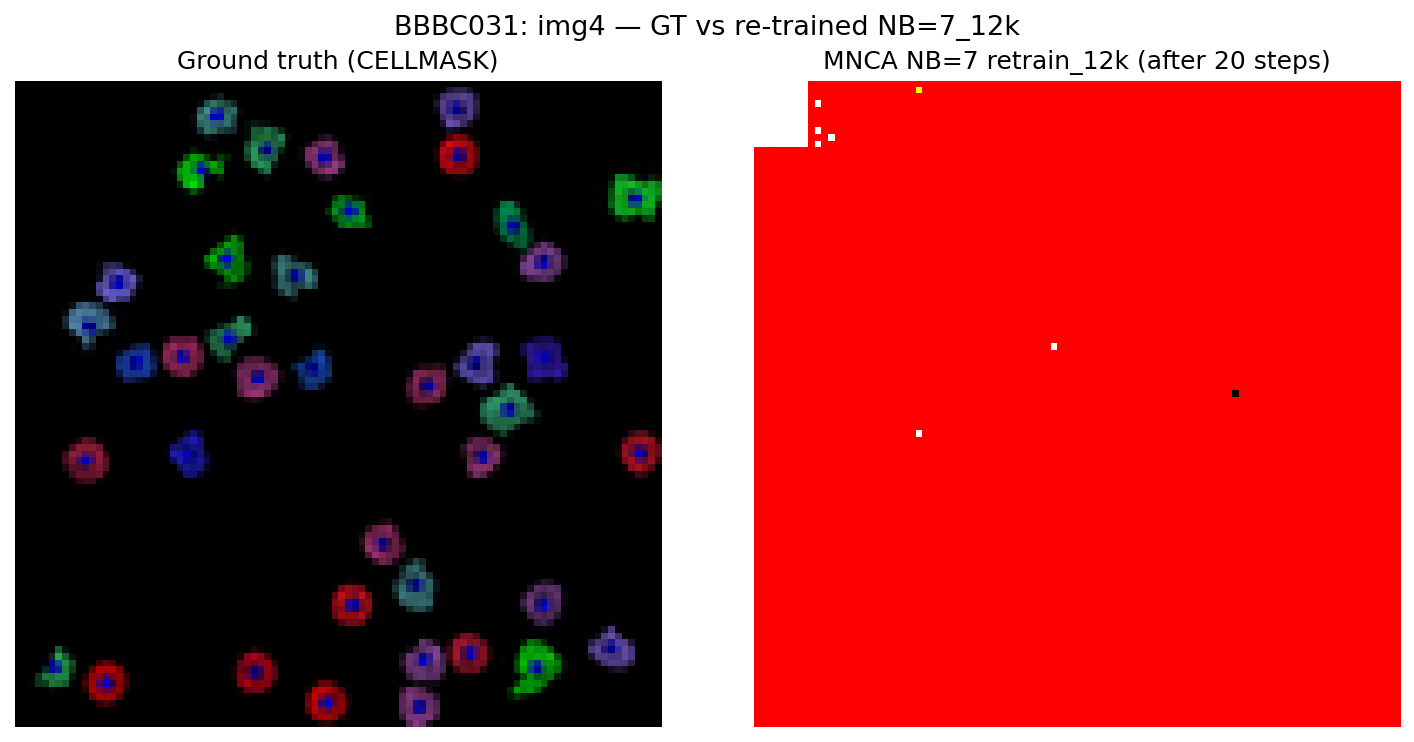
\includegraphics[width=\textwidth]{figs/bbbc031/bbbc031_gt_vs_mnca_NB7_retrain_12k_img4.png}
    \caption*{img4}
  \end{minipage}\hfill
  \caption{BBBC031: outputs from \(NB=7\) extended re-training (12\,000 steps). \textbf{Legend:} five panels = img0--img4; each = ground truth vs.\ prediction after 20 simulation steps.}
  \label{fig:impl:bbbc031:gt_vs_nb7_retrain_12k}
\end{figure}

\subsection{Interpretation}

Overall, the BBBC031 segmentation experiment mirrors the broader thesis theme that \textbf{larger neighbourhoods can be harder to optimise} unless training schedules are adapted.
Within this in-sample setting, \(NB=3\) reaches near-perfect overlap metrics under the default schedule, while \(NB=7\) is substantially more sensitive to the learning rate and the length of optimisation.
The re-training and extended re-training runs show that \(NB=7\) can be made stable and can close the gap on some images, but that the outcome is image-dependent under the explored schedules.

%-------------------------------------------------------------------
\section{Thesis takeaway}
\label{sec:results:takeaway}
%-------------------------------------------------------------------

The main takeaway of this thesis is that MNCA can model tissue-like dynamics in a controlled synthetic setting, but careful experimental design is required to obtain interpretable conclusions.
In particular, the neighbourhood-size effect can be masked by training/evaluation confounds when models already fail at long-horizon rollouts.
Under the controlled sweep, neighbourhood size has a statistically significant effect (Kruskal--Wallis \(p < 10^{-4}\)); beyond a minimal receptive field (\(NB \ge 2\)), no single \(NB\) is best on every metric.
The evaluation protocol (especially alignment between training and free-rollout evaluation and the use of multiple rollout horizons) is central to observing and interpreting these effects; limitations and threats to validity are discussed in \cref{sec:impl:threats}.
